% report.tex — Laporan: koordinasi fault tolerance lintas-lapis BEAM/OTP <-> Kubernetes
% Kompilasi (XeLaTeX, karena memakai fontspec):
%   xelatex report  &&  bibtex report  &&  xelatex report  &&  xelatex report

\documentclass[11pt,a4paper]{report}

% --- Font: Noto Serif untuk teks utama, JetBrains Mono untuk kode/lstlisting ---
\usepackage{fontspec}
\setmainfont{Noto Serif}
\newfontfamily\notosans{Noto Sans}
\setmonofont{JetBrains Mono}[Scale=0.92]

\usepackage[bahasa]{babel}
\usepackage[a4paper,margin=2.5cm]{geometry}
\usepackage{graphicx}
\usepackage{booktabs}
\usepackage{amsmath}
\usepackage{amssymb}
\usepackage{xcolor}
\usepackage{enumitem}
\usepackage{float}
\usepackage{caption}
\captionsetup{labelfont=bf}
\usepackage{listings}
\usepackage{algorithm}
\usepackage{algpseudocode}
\floatname{algorithm}{Algoritma}
\usepackage{hyperref}
\hypersetup{
  colorlinks=true,
  linkcolor={blue!55!black},
  citecolor={green!45!black},
  urlcolor={magenta!70!black},
}

\graphicspath{{assets/}{../diagrams/problems/}{../diagrams/mechanisms/}{../diagrams/}}

% --- Gaya listing (memakai JetBrains Mono via \ttfamily) ---
\definecolor{codebg}{HTML}{F6F8FA}
\definecolor{codekw}{HTML}{0B5FA5}
\definecolor{codecm}{HTML}{6A737D}
\definecolor{codestr}{HTML}{1A7F37}
\lstset{
  basicstyle=\ttfamily\small,
  backgroundcolor=\color{codebg},
  keywordstyle=\color{codekw}\bfseries,
  commentstyle=\color{codecm}\itshape,
  stringstyle=\color{codestr},
  frame=single, framesep=5pt, rulecolor=\color{gray!35},
  breaklines=true, showstringspaces=false, columns=fullflexible,
  numbers=left, numberstyle=\ttfamily\footnotesize\color{gray!70},
  xleftmargin=2.2em,
  keywords={defmodule,def,defp,do,end,use,fn,case,cond,Supervisor,GenServer,start_link,init,children,strategy}
}

\newcommand{\todo}[1]{\textcolor{red}{[CATATAN: #1]}}
% kotak centang untuk checklist (selesai / belum)
\newcommand{\cbtodo}{\ensuremath{\square}}
\newcommand{\cbdone}{\rlap{\hspace{0.12em}\raisebox{0.25ex}{\scriptsize\ensuremath{\checkmark}}}\ensuremath{\square}}

\title{\textbf{Mengoordinasikan Dua Lapis Self-Healing:}\\[4pt]
Toleransi Kesalahan Lintas-Lapis antara Runtime BEAM dan Kubernetes}
\author{Alfa Yohannis\\ Universitas Pradita \\ \texttt{alfa.ryano@pradita.ac.id}}
\date{\today}

\begin{document}
\maketitle

\begin{abstract}
\noindent Sistem Elixir berbasis cloud memuat dua mekanisme toleransi kesalahan yang
saling tumpang tindih namun bekerja independen: supervisi OTP pada lapis \emph{runtime}
bahasa dan \emph{self-healing} Kubernetes pada lapis orkestrasi. Masing-masing
efektif jika berdiri sendiri, tetapi karena tidak berkoordinasi, keduanya memunculkan
ragam kegagalan di perbatasannya---\emph{probe} yang salah melaporkan VM yang macet,
pemulihan ganda yang mubazir, lalu lintas yang diarahkan ke node yang belum bergabung ke
\emph{cluster}, kehilangan state ketika \emph{handoff} pada \emph{graceful shutdown}
melampaui \emph{grace period}, serta \emph{split-brain} yang tak terlihat oleh
orkestrator. Laporan ini mengarakterisasi celah koordinasi tersebut, mengusulkan sebuah
protokol koordinasi lintas-lapis yang memberi supervisor OTP dan pengendali Kubernetes
sebuah kontrak kepemilikan dan \emph{handoff} yang jelas, lalu mengevaluasinya melalui
injeksi kesalahan terhadap \emph{baseline} tanpa koordinasi. \todo{1--2 kalimat hasil
utama setelah evaluasi.} Kami juga menunjukkan bahwa celah ini berlaku lintas
\emph{actor runtime}: tumpukan JVM/Akka sudah menyediakan sebagian \emph{plumbing}-nya,
tumpukan BEAM belum, dan belum ada platform yang memformalkan koordinasi tersebut
sebagai dua \emph{control loop} yang saling berinteraksi.
\end{abstract}

\tableofcontents

\chapter{Pendahuluan}
\label{ch:intro}
Baik runtime BEAM/OTP maupun Kubernetes sama-sama memiliki mekanisme \emph{self-healing} bawaan,
namun keduanya beroperasi pada granularitas yang berbeda: OTP memulihkan kegagalan pada
tingkat \emph{process} di dalam satu VM, sedangkan Kubernetes memulihkan kegagalan pada
tingkat \emph{pod}/\emph{node}. Karena keduanya tidak saling berbicara secara baku,
interaksinya di perbatasan justru memunculkan masalah yang tidak dialami masing-masing
lapis ketika bekerja sendiri. \todo{perkuat motivasi dengan laporan praktik dan isu
\emph{rolling update} pada Akka.}

\noindent Kontribusi laporan ini:
\begin{itemize}[nosep]
  \item Taksonomi komunikasi BEAM$\leftrightarrow$Kubernetes yang diperlukan, serta katalog
        lima \emph{titik gesekan} runtime-vs-orkestrator (Bab~\ref{ch:problems}).
  \item Sebuah protokol koordinasi lintas-lapis antara supervisor OTP dan pengendali
        Kubernetes (Bab~\ref{ch:design}).
  \item Evaluasi melalui injeksi kesalahan terhadap \emph{baseline} tanpa koordinasi
        (Bab~\ref{ch:eval}).
  \item Bukti bahwa celah ini dan solusi parsialnya bersifat umum lintas \emph{actor
        runtime} (Bab~\ref{ch:disc}).
\end{itemize}

\chapter{Latar Belakang}
\label{ch:background}
\textbf{Supervisi OTP.} Pada BEAM, kegagalan ditangani dengan filosofi ``\emph{let it
crash}'': sebuah \emph{supervisor} memantau anak-anaknya dan menyalakannya ulang menurut
strategi tertentu bila terjadi \emph{crash}. Batas intensitas \emph{restart} diatur oleh
\texttt{max\_restarts}/\texttt{max\_seconds}.

\begin{lstlisting}[caption={Contoh \emph{supervision tree} OTP sederhana.}, label={lst:sup}]
defmodule MyApp.Supervisor do
  use Supervisor

  def start_link(arg) do
    Supervisor.start_link(__MODULE__, arg, name: __MODULE__)
  end

  def init(_arg) do
    children = [
      {MyApp.Worker, []},
      {MyApp.Cache, []}
    ]
    Supervisor.init(children, strategy: :one_for_one, max_restarts: 3, max_seconds: 5)
  end
end
\end{lstlisting}

Listing~\ref{lst:sup} memperlihatkan sebuah \emph{supervisor} berstrategi
\texttt{:one\_for\_one} yang mengawasi dua anak (\texttt{Worker} dan \texttt{Cache}):
bila salah satu anak \emph{crash}, hanya anak itu yang disalakan ulang; bila intensitas
\emph{restart} melampaui \texttt{max\_restarts} dalam rentang \texttt{max\_seconds},
supervisor menghentikan dirinya sehingga kegagalan tereskalasi ke induknya. Perilaku
eskalasi inilah yang kelak berbenturan dengan \emph{restart} pada tingkat \emph{pod}
(Bab~\ref{ch:problems}).

\noindent\textbf{Kubernetes.} Kubernetes mengelola siklus hidup \emph{pod} melalui
\emph{liveness}/\emph{readiness probe}, pengendali (\emph{controller}),
\emph{PodDisruptionBudget} (PDB)~\cite{k8sPDB}, dan \emph{graceful shutdown}
(\texttt{SIGTERM} + \texttt{terminationGracePeriodSeconds}). Penskalaan berbasis metrik
aplikasi dapat dilakukan dengan KEDA~\cite{keda}.

\noindent\textbf{Klastering BEAM.} Di atas Kubernetes, pembentukan \emph{cluster} BEAM
lazim memakai libcluster~\cite{libcluster}, sementara Horde~\cite{horde} menyediakan
\emph{supervisor}/\emph{registry} terdistribusi dengan \emph{handoff} proses. Untuk
menulis \emph{operator} Kubernetes dalam Elixir tersedia Bonny~\cite{bonny}.

% readme.tex — \input dari report.tex (sumber: README proyek)
\section{Komunikasi BEAM--Kubernetes: Kapan Diperlukan?}
\label{sec:komunikasi}

Misalkan sebuah aplikasi Elixir berjalan di dalam sebuah \emph{pod}. Kapan komunikasi
antara runtime BEAM dan Kubernetes benar-benar \emph{diperlukan}? Pertanyaan ini
menyangkut lalu lintas yang melintasi perbatasan antara \emph{control plane} Kubernetes
dan runtime BEAM. Lalu lintas tersebut mengalir dalam tiga arah: (i)~\emph{K8s
$\rightarrow$ Elixir}, ketika \emph{control plane} memberi sinyal atau konfigurasi ke
aplikasi; (ii)~\emph{Elixir $\rightarrow$ API K8s}, ketika aplikasi mengueri atau
mengendalikan \emph{cluster}; dan (iii)~\emph{Elixir $\leftrightarrow$ Elixir melalui
K8s}, ketika antar-\emph{pod} saling menemukan untuk membentuk \emph{cluster} BEAM.

Inti pemahamannya: untuk aplikasi \emph{stateless} sederhana, hampir tidak ada komunikasi
yang diperlukan---BEAM berjalan, supervisor OTP menyalakan ulang \emph{process} yang
\emph{crash}, dan Kubernetes me-\emph{restart} \emph{pod} bila seluruh VM mati. Kebutuhan
komunikasi muncul pada situasi spesifik yang dipetakan oleh lima kategori berikut.

\section{Lima Kategori Komunikasi}
\label{sec:kategori}
\begin{description}[leftmargin=2.2em,style=nextline]
  \item[A. Pembentukan \emph{cluster} \& penemuan \emph{peer} (Elixir$\leftrightarrow$Elixir via K8s).]
    Distribusi BEAM perlu mengetahui alamat node lain, sementara IP \emph{pod} bersifat
    fana; penemuan harus berasal dari Kubernetes melalui libcluster~\cite{libcluster}
    (API atau DNS \emph{headless service}). Contoh kebutuhan: \emph{Phoenix.PubSub},
    \emph{Presence}, Horde~\cite{horde}, \emph{singleton} global, cache terdistribusi.
  \item[B. Sinyal siklus hidup \& kesehatan \emph{pod} (K8s$\rightarrow$Elixir).]
    \emph{Liveness}/\emph{readiness probe}, \emph{graceful shutdown} via \texttt{SIGTERM}
    dengan \emph{draining} dan \emph{handoff}, serta \emph{preStop hook}.
  \item[C. Injeksi konfigurasi \& identitas (K8s$\rightarrow$Elixir).]
    \emph{ConfigMap}, \emph{Secret} (termasuk \emph{cookie} distribusi Erlang yang harus
    seragam antar-\emph{pod}), dan \emph{Downward API} (\texttt{POD\_IP}, \texttt{POD\_NAME})
    untuk menyusun \texttt{RELEASE\_NODE}.
  \item[D. Observabilitas \& sinyal penskalaan (Elixir$\rightarrow$ekosistem K8s).]
    Metrik Prometheus yang memberi makan HPA/KEDA~\cite{keda}; penskalaan mengubah jumlah
    \emph{pod} sehingga memicu ulang kategori A dan B.
  \item[E. Kontrol aktif \emph{cluster} (Elixir$\rightarrow$API K8s).]
    Pola \emph{operator}: aplikasi mengendalikan Kubernetes sendiri, mis.\ dengan
    Bonny~\cite{bonny} (mengawasi CRD, membuat \emph{Job}/\emph{Pod}, \emph{leader
    election} via \emph{Lease}).
\end{description}

\section{Pembagian Peran: OTP vs.\ Kubernetes}
\label{sec:overlap}
Kedua lapis bersifat saling melengkapi, bukan redundan, karena bekerja pada granularitas
berbeda (Tabel~\ref{tab:overlap}). Keduanya tidak berbicara secara baku; kebutuhan
komunikasi justru muncul tepat ketika peran mereka beririsan---itulah sumber lima
permasalahan pada Bab~\ref{ch:problems}.

\begin{table}[H]
  \centering\small
  \begin{tabular}{@{}p{0.20\linewidth}p{0.36\linewidth}p{0.36\linewidth}@{}}
    \toprule
    & \textbf{Supervisi OTP} & \textbf{Kubernetes} \\
    \midrule
    Granularitas & \emph{Process} (dalam VM) & Kontainer / \emph{pod} / \emph{node} \\
    Pulih dari & Bug logika, gangguan sesaat & OOM, matinya \emph{node}, \emph{image} buruk \\
    Kecepatan & mikro--milidetik & detik--menit \\
    State & Dibangun ulang sesuai strategi & \emph{Pod} diganti utuh \\
    \bottomrule
  \end{tabular}
  \caption{Pembagian peran antara supervisi runtime (OTP) dan orkestrator (Kubernetes).}
  \label{tab:overlap}
\end{table}


% ---- Bab-bab terpisah ----
% problems.tex — \input dari report.tex
\chapter{Permasalahan Koordinasi}
\label{ch:problems}

Karena kedua lapis pemulihan beroperasi pada granularitas berbeda dan tidak berbicara
secara baku, interaksinya memunculkan lima \emph{titik gesekan}. Setiap masalah disajikan
dengan: konteks skenario, diagram \emph{sekuens} (pertukaran pesan antar-komponen),
diagram \emph{aktivitas} (alur keputusan), pseudokode, lalu pembahasan yang menelusuri
ketiganya. Warna merah menandai jalur kegagalan, hijau menandai jalur yang diinginkan.
Tiap masalah dikonkretkan dengan aplikasi \emph{ilustratif} yang sengaja
direka---\emph{PayGate}, \emph{SensorHub}, \emph{ArenaServer}, \emph{CoEdit}, dan
\emph{TopScore}---bukan produk nyata, melainkan contoh hipotetis untuk membumikan
persoalan.

\section{Ketidakcocokan Granularitas \emph{Liveness}}
\label{sec:p1}
Layanan \emph{webhook} pembayaran \emph{PayGate} menilai tiap transaksi melalui API
penilai \emph{fraud} eksternal lewat \emph{pool} Finch---pustaka klien HTTP Elixir yang
mengelola sekumpulan koneksi keluar yang dipakai ulang. Ketika API tersebut menggantung
(TCP setengah terbuka, tanpa \emph{timeout}), seluruh pekerja \emph{pool} terblokir dan
semua permintaan macet, tetapi \emph{listener} Cowboy---server HTTP Phoenix yang menerima
koneksi pada \emph{port}---tetap meng-\emph{accept} \emph{socket} sehingga \emph{probe} TCP
lulus dan Kubernetes mengira \emph{pod} sehat. Sebaliknya, \emph{probe} yang terlalu agresif
justru membunuh VM yang sebenarnya akan dipulihkan OTP.

\begin{figure}[H]\centering\includegraphics[width=\linewidth,height=0.9\textheight,keepaspectratio]{01-liveness-mismatch-sequence}
  \caption{Masalah 1 (sekuens): jalur sebuah permintaan ke \emph{PayGate}. Cowboy tetap
  menerima koneksi TCP dan pekerja Finch terblokir pada API \emph{fraud} yang menggantung;
  karena \emph{probe} hanya menguji penerimaan \emph{socket}, ia lulus meski 100\%
  pembayaran macet.}\label{fig:p1-seq}\end{figure}
\begin{figure}[H]\centering\includegraphics[width=\linewidth,height=0.9\textheight,keepaspectratio]{01-liveness-mismatch-activity}
  \caption{Masalah 1 (aktivitas): dua mode kegagalan rancangan \emph{probe}. \emph{Probe}
  dangkal melewatkan subsistem yang macet (negatif palsu); \emph{probe} agresif dengan
  \texttt{failureThreshold} rendah membunuh VM yang sebenarnya dapat dipulihkan OTP
  (positif palsu).}\label{fig:p1-act}\end{figure}
\begin{algorithm}[H]\caption{Masalah 1 --- \emph{probe} TCP naif.}\label{alg:p1}
\begin{algorithmic}[1]
\Function{NaiveProbe}{}
  \If{\Call{TcpAccept}{\textit{port}}} \State \Return \textit{HEALTHY} \Comment{meski \emph{pool} macet} \EndIf
\EndFunction
\end{algorithmic}\end{algorithm}

\noindent\textbf{Pembahasan.} Diagram sekuens (Gambar~\ref{fig:p1-seq}) menelusuri satu
transaksi: \emph{Client}~$\rightarrow$~Cowboy~$\rightarrow$~Finch~$\rightarrow$~API
\emph{fraud}, lalu API menggantung sehingga pekerja tak pernah dibebaskan. Pesan
\emph{probe} dari kubelet yang datang sesudahnya tetap dibalas ``\emph{ACK}'' oleh Cowboy
karena penerimaan \emph{socket} berada di jalur yang berbeda dari \emph{pool} yang macet.
Diagram aktivitas (Gambar~\ref{fig:p1-act}) memisahkan persoalan menjadi dua cabang
keputusan rancangan: cabang ``\emph{probe} dangkal'' berhenti pada ``\emph{port} terbuka?''
sehingga melewatkan kemacetan internal, sedangkan cabang ``\emph{probe} agresif'' bercabang
pada \texttt{failureThreshold} yang terlalu kecil dan mematikan VM saat gangguan sesaat.
Algoritma~\ref{alg:p1} memformalkan akarnya: vonis \textit{HEALTHY} pada baris~2 hanya
bergantung pada \textsc{TcpAccept}, tanpa sama sekali menyentuh keadaan \emph{pool} pekerja
atau \emph{supervision tree}---inilah celah semantik yang ditutup M1 dan M9.

\subsection{Ilustrasi Sederhana}
\label{subsec:p1-ilustrasi}
Aplikasi \emph{PayGate} memanggil API \emph{fraud} lewat \emph{connection pool} (sekumpulan
koneksi siap-pakai ke layanan luar). Langkahnya:
\begin{enumerate}[nosep,leftmargin=2em]
  \item API \emph{fraud} menggantung---tidak membalas dan tanpa batas waktu---sehingga satu
        per satu pekerja di \emph{pool} ikut menunggu selamanya, hingga semua pekerja habis
        dan setiap pembayaran macet.
  \item Pada saat yang sama, kubelet (agen Kubernetes di tiap node yang menjalankan
        pemeriksaan kesehatan) mengirim \emph{probe} TCP: ia hanya mengecek apakah \emph{port}
        4000 mau menerima koneksi.
  \item Karena server web (Cowboy) tetap menerima koneksi di \emph{port} itu---menerima
        koneksi adalah pekerjaan yang terpisah dari memprosesnya---\emph{probe} lulus, dan
        Kubernetes menyimpulkan \emph{pod} sehat.
\end{enumerate}
\noindent Akar masalahnya: \emph{probe} hanya bertanya ``\emph{port}-nya hidup?'', bukan
``aplikasinya masih mengerjakan sesuatu?''. Inilah yang diperbaiki M1 dan M9.

\section{Pemulihan Ganda}
\label{sec:p2}
Pada \emph{ingester} telemetri IoT \emph{SensorHub}, sebuah \emph{frame} cacat membuat
\emph{decoder}---sebuah \texttt{GenServer} (proses \emph{stateful} Elixir)---terus
\emph{crash}. Bila \texttt{max\_restarts} (jatah \emph{restart} yang dipantau supervisor)
terlalu longgar,
\emph{process} ber-\emph{crash-loop} tanpa terlihat oleh Kubernetes; bila diatur wajar,
habisnya jatah \emph{restart} mengeskalasikan kegagalan ke Kubernetes (\emph{CrashLoopBackOff})
secara sengaja.

\begin{figure}[H]\centering\includegraphics[width=\linewidth,height=0.9\textheight,keepaspectratio]{02-double-recovery-sequence}
  \caption{Masalah 2 (sekuens): perangkat mengirim ulang \emph{frame} cacat sehingga
  \emph{decoder} \emph{crash} berulang. Bila jatah \emph{restart} longgar, \emph{loop}
  tak terlihat oleh Kubernetes; bila wajar, supervisor menghentikan diri dan VM keluar
  sehingga Kubernetes mengambil alih.}\label{fig:p2-seq}\end{figure}
\begin{figure}[H]\centering\includegraphics[width=\linewidth,height=0.9\textheight,keepaspectratio]{02-double-recovery-activity}
  \caption{Masalah 2 (aktivitas): batas eskalasi kepemilikan. Selama dalam jatah, OTP
  yang memulihkan; saat jatah habis, kepemilikan berpindah ke Kubernetes.}\label{fig:p2-act}\end{figure}
\begin{algorithm}[H]\caption{Masalah 2 --- pemulihan tak terkoordinasi.}\label{alg:p2}
\begin{algorithmic}[1]
\Procedure{OnCrash}{\textit{child}}
  \State \Call{OTP.Restart}{\textit{child}} \Comment{max\_restarts longgar $\Rightarrow$ loop tak terlihat}
  \State \textbf{// VM tetap hidup; Kubernetes tidak diberi tahu}
\EndProcedure
\end{algorithmic}\end{algorithm}

\noindent\textbf{Pembahasan.} Diagram sekuens (Gambar~\ref{fig:p2-seq}) memperlihatkan
\emph{loop} berulang \emph{Device}~$\rightarrow$~\emph{Decoder}~$\rightarrow$~Supervisor:
perangkat mengirim ulang \emph{frame} yang sama, \emph{decoder} \emph{crash}, supervisor
menyalakannya ulang, lalu siklus berputar. Pada cabang ``jatah longgar'', tidak ada satu
pun pesan yang mengalir ke Kubernetes---itulah sebabnya kegagalan menjadi tak terlihat.
Diagram aktivitas (Gambar~\ref{fig:p2-act}) menempatkan keputusan kunci pada ``apakah
intensitas \emph{restart} melampaui jatah?''; selama \emph{tidak}, OTP yang memiliki
kegagalan, dan begitu \emph{ya}, kepemilikan berpindah ke Kubernetes melalui keluarnya VM.
Algoritma~\ref{alg:p2} sengaja ditulis ``naif'': baris~2 selalu me-\emph{restart} tanpa
memeriksa jatah, dan komentar baris~3 menyorot bahwa lapis orkestrator tak pernah
diberi tahu---persis ketiadaan kebijakan kepemilikan yang ditangani M2.

\subsection{Ilustrasi Sederhana}
\label{subsec:p2-ilustrasi}
Pada \emph{SensorHub}:
\begin{enumerate}[nosep,leftmargin=2em]
  \item Sebuah \emph{frame} (paket data) yang rusak dari perangkat membuat \emph{decoder}
        (\emph{process} yang menerjemahkan data masuk) \emph{crash}.
  \item Supervisor (\emph{process} pengawas yang otomatis menyalakan ulang anaknya saat
        \emph{crash}) langsung menghidupkannya kembali; perangkat mengirim ulang \emph{frame}
        rusak yang sama, \emph{decoder} \emph{crash} lagi, dihidupkan lagi---berputar terus.
  \item Selama VM BEAM tetap hidup, Kubernetes tak melihat masalah apa pun (\emph{probe}
        lulus) sehingga diam saja. Bila jatah \emph{restart} (\texttt{max\_restarts}) diatur
        wajar, supervisor akhirnya menyerah dan VM keluar, barulah Kubernetes me-\emph{restart}
        \emph{pod}.
\end{enumerate}
\noindent Akar masalahnya: tak ada kesepakatan lapis mana yang ``memiliki'' kegagalan ini,
sehingga bisa terjadi pemulihan berulang yang sia-sia. Ditangani M2 dan M8.

\section{\emph{Readiness} vs.\ Pembentukan \emph{Cluster}}
\label{sec:p3}
Pada \emph{backend} permainan \emph{ArenaServer}, tiap pertandingan adalah \emph{singleton}
global yang dikelola Horde (\emph{registry}/\emph{supervisor} terdistribusi dengan
\emph{handoff}). Saat \emph{rolling deploy}, sebuah \emph{pod} baru ditandai siap (hanya
karena \emph{port} terbuka) sebelum libcluster (pembentuk \emph{cluster} BEAM) menemukan
\emph{peer} dan Horde tersinkron;
lalu lintas tiba terlalu dini dan \emph{registry} masih kosong.

\begin{figure}[H]\centering\includegraphics[width=\linewidth,height=0.9\textheight,keepaspectratio]{03-readiness-cluster-sequence}
  \caption{Masalah 3 (sekuens): \emph{pod} menandai diri siap segera setelah \emph{port}
  terbuka, lalu Kubernetes merutekan permintaan pemain sebelum Horde tersinkron sehingga
  pencarian \emph{singleton} menemui \emph{registry} kosong.}\label{fig:p3-seq}\end{figure}
\begin{figure}[H]\centering\includegraphics[width=\linewidth,height=0.9\textheight,keepaspectratio]{03-readiness-cluster-activity}
  \caption{Masalah 3 (aktivitas): perbandingan kebijakan \emph{gating readiness}---``\emph{port}
  terbuka'' (terlalu dini) vs.\ ``\emph{cluster} tergabung dan Horde konvergen''
  (benar).}\label{fig:p3-act}\end{figure}
\begin{algorithm}[H]\caption{Masalah 3 --- \emph{readiness} terlalu dini.}\label{alg:p3}
\begin{algorithmic}[1]
\Procedure{OnPodStart}{}
  \State \Call{BindPort}{4000}; \Call{MarkReady}{} \Comment{libcluster/Horde belum konvergen}
\EndProcedure
\Procedure{OnRequest}{\textit{match}}
  \State \Call{Lookup}{\textit{match}} \Comment{$\rightarrow$ notFound / duplikat}
\EndProcedure
\end{algorithmic}\end{algorithm}

\noindent\textbf{Pembahasan.} Diagram sekuens (Gambar~\ref{fig:p3-seq}) menyusun urutan
waktu yang kritis: \emph{pod} mengikat \emph{port}, kubelet mengirim \emph{probe} TCP yang
langsung lulus, Kubernetes menambahkan \emph{pod} ke \emph{Endpoints}, lalu permintaan
pemain tiba---semua \emph{sebelum} pesan penemuan libcluster dan sinkronisasi Horde
selesai. Diagram aktivitas (Gambar~\ref{fig:p3-act}) mengontraskan dua kebijakan
\emph{gating}: jalur ``\emph{port} terbuka'' langsung menandai siap, sedangkan jalur yang
benar menunggu syarat gabungan ``\emph{cluster} tergabung \emph{dan} Horde konvergen''.
Algoritma~\ref{alg:p3} memisahkan dua prosedur: \textsc{OnPodStart} (baris~2) menandai
siap segera setelah \textsc{BindPort}, sementara \textsc{OnRequest} (baris~5) melakukan
\textsc{Lookup} yang mengembalikan \emph{notFound} atau bahkan mendaftarkan \emph{singleton}
duplikat---akibat langsung dari penandaan siap yang prematur, yang diperbaiki M4.

\subsection{Ilustrasi Sederhana}
\label{subsec:p3-ilustrasi}
\emph{ArenaServer} adalah \emph{backend} sebuah permainan daring \emph{real-time} berbasis
pertandingan---bayangkan game pertarungan arena (sejenis MOBA atau \emph{battle royale})
tempat banyak pemain bermain bersama dalam satu pertandingan. Tiap pertandingan yang sedang
berlangsung diwakili oleh satu \emph{process} di BEAM yang menyimpan keadaan permainan (skor,
posisi pemain, dan sebagainya).

Karena pemain berdatangan melalui \emph{load balancer}, dua pemain dalam pertandingan yang
sama bisa saja tersambung ke \emph{pod} yang berbeda. Agar keduanya tetap dilayani oleh
\emph{process} pertandingan yang sama, \emph{pod}-\emph{pod} itu harus saling mengenal dan
membentuk satu \emph{cluster} BEAM---\textbf{inilah mengapa \emph{peer} diperlukan}: tanpa
mengetahui rekan-rekannya, sebuah \emph{pod} tak bisa menemukan pertandingan yang sebenarnya
berjalan di \emph{pod} lain. \textbf{Mengapa perlu sinkronisasi}: daftar ``pertandingan~$X$
berjalan di \emph{pod}~$Y$'' harus diketahui seragam oleh semua \emph{pod}, dan Horde menjaga
daftar (\emph{registry}) ini tetap tersinkron sehingga tiap \emph{pod} dapat mengarahkan
pemain ke tempat yang benar. \textbf{Mengapa perlu \emph{rolling deploy}}: memperbarui game
(versi baru, perbaikan bug) dilakukan bertahap agar layanan tetap hidup tanpa
\emph{downtime}; \emph{pod} lama diganti \emph{pod} baru sedikit demi sedikit---dan di sinilah
\emph{pod} baru bermunculan, yang harus bergabung ke \emph{cluster} lebih dulu sebelum layak
melayani. Masalahnya muncul pada langkah berikut:
\begin{enumerate}[nosep,leftmargin=2em]
  \item Sebuah \emph{pod} baru dinyalakan; ia mengikat \emph{port} dan langsung menandai
        diri ``siap'' (\emph{ready}) semata karena \emph{port}-nya terbuka.
  \item Kubernetes pun mengarahkan pemain ke \emph{pod} itu---padahal \emph{pod} belum
        bergabung ke \emph{cluster}: libcluster (yang menemukan antar-\emph{pod}) belum
        menemukan rekan, dan \emph{registry} Horde belum tersinkron.
  \item Ketika pemain mencari pertandingannya (yang dipegang sebagai \emph{singleton}---satu
        \emph{process} unik untuk pertandingan itu di seluruh \emph{cluster}), \emph{pod} ini
        tak menemukannya (\emph{registry}-nya masih kosong), lalu menjawab ``pertandingan
        tak ada'' atau malah membuat \emph{process} duplikat yang memecah pertandingan.
\end{enumerate}
\noindent Akar masalahnya: ``siap'' ditandai terlalu dini---\emph{port} terbuka belum berarti
siap melayani karena \emph{cluster} belum terbentuk. Diperbaiki M4, yang menahan status
``siap'' sampai \emph{pod} benar-benar tergabung dan \emph{registry} tersinkron.

\section{Churn \emph{Rolling-Deploy}: \emph{Handoff} vs.\ \emph{Grace Period}}
\label{sec:p4}
Pada editor kolaboratif \emph{CoEdit}, tiap dokumen adalah \emph{process} \emph{stateful}
ber-CRDT (\emph{conflict-free replicated data type}---struktur data yang konvergen tanpa
koordinasi) yang di-\emph{handoff} via Horde. Ketika \texttt{SIGTERM} tiba, \emph{handoff}
ratusan \emph{process} memerlukan waktu lebih lama daripada
\texttt{terminationGracePeriodSeconds}; saat \texttt{SIGKILL} datang, dokumen yang belum
berpindah mati bersama suntingan yang belum tersinkron.

\begin{figure}[H]\centering\includegraphics[width=\linewidth,height=0.9\textheight,keepaspectratio]{04-rolling-deploy-sequence}
  \caption{Masalah 4 (sekuens): setelah \texttt{SIGTERM}, \emph{pod} men-\emph{drain} dan
  memulai \emph{handoff} 400 \emph{process}; karena \emph{handoff} ($\approx$45\,s)
  melampaui \emph{grace} (30\,s), \texttt{SIGKILL} memutus sisanya dan state hilang.}\label{fig:p4-seq}\end{figure}
\begin{figure}[H]\centering\includegraphics[width=\linewidth,height=0.9\textheight,keepaspectratio]{04-rolling-deploy-activity}
  \caption{Masalah 4 (aktivitas): perlombaan antara penyelesaian \emph{drain}/\emph{handoff}
  dan tenggat \emph{grace period}; bila tenggat menang, terjadi kehilangan state.}\label{fig:p4-act}\end{figure}
\begin{algorithm}[H]\caption{Masalah 4 --- \emph{handoff} melampaui \emph{grace}.}\label{alg:p4}
\begin{algorithmic}[1]
\Procedure{OnSigterm}{}
  \State \Call{StartGraceTimer}{30}
  \For{$p \in \{400\ \text{proc}\}$} \State \Call{Handoff}{$p$} \Comment{$\approx$45 s} \EndFor
  \If{\textbf{not} \Call{Done}{} \textbf{before} \textit{deadline}} \State \Call{Sigkill}{} \Comment{state hilang} \EndIf
\EndProcedure
\end{algorithmic}\end{algorithm}

\noindent\textbf{Pembahasan.} Diagram sekuens (Gambar~\ref{fig:p4-seq}) menelusuri jalur
terminasi: \emph{Deployment}~$\rightarrow$~kubelet mengirim \texttt{SIGTERM}, \emph{pod}
men-\emph{drain} \emph{endpoint} lalu mengalirkan 400 perintah \emph{handoff} ke node
tersisa; sebuah pesan \texttt{SIGKILL} terjadwal di $t{=}30$\,s memotong aliran yang baru
mencapai $\approx$45\,s. Diagram aktivitas (Gambar~\ref{fig:p4-act}) memodelkan ini sebagai
perlombaan: percabangan ``\emph{handoff} selesai sebelum tenggat?'' menentukan apakah
keluar bersih atau \texttt{SIGKILL}. Algoritma~\ref{alg:p4} memperjelas ketakcocokan
waktu: baris~2 memulai pewaktu 30\,s, perulangan baris~3 melakukan 400 \emph{handoff}
yang totalnya $\approx$45\,s, dan kondisi baris~4 memicu \textsc{Sigkill} begitu tenggat
terlewati---ketiadaan kopling antara durasi \emph{handoff} dan \emph{grace} inilah yang
dijembatani M3.

\subsection{Ilustrasi Sederhana}
\label{subsec:p4-ilustrasi}
Untuk pembaca yang baru mengenal Kubernetes, alur masalah ini ditelusuri langkah demi
langkah dengan angka konkret. Misalkan sebuah \emph{pod} (wadah berisi satu salinan aplikasi
yang dijadwalkan dan dikelola Kubernetes) menjalankan 400 \emph{process} (unit eksekusi
sangat ringan di dalam VM BEAM---mesin virtual tempat Elixir berjalan---sehingga satu
aplikasi lazim menjalankan ratusan ribu sekaligus, berbeda dari proses sistem operasi yang
``berat''), dan tiap \emph{process} memegang \emph{state}: data yang sedang ditahannya di
memori, di sini suntingan dokumen yang belum tersimpan ke basis data. Ketika Kubernetes
memutuskan mematikan \emph{pod} ini (misalnya karena \emph{rolling update}, yakni pembaruan
bertahap yang mengganti \emph{pod} satu per satu ketika ada versi baru aplikasi, perubahan
konfigurasi, atau pembaruan lain), terjadi rangkaian berikut (Tabel~\ref{tab:p4-timeline}):

\begin{enumerate}[nosep,leftmargin=2em]
  \item Pada detik ke-0, Kubernetes mengirim \texttt{SIGTERM} (sinyal yang meminta proses
        berhenti dengan sopan---aplikasi masih diberi kesempatan membereskan diri lebih
        dulu) dan memulai pewaktu \emph{grace} (jatah waktu agar aplikasi sempat selesai
        sebelum dimatikan paksa) selama 30~detik; \emph{pod} lalu berhenti menerima koneksi
        baru (disebut \emph{drain}---menuntaskan permintaan yang sedang berjalan sambil
        menolak yang baru).
  \item \emph{Pod} mulai memindahkan ke-400 \emph{process} beserta \emph{state}-nya ke node
        lain (mesin lain---fisik atau virtual---tempat \emph{pod} dijalankan, satu dari
        banyak node dalam \emph{cluster}) melalui \emph{handoff} (pemindahan \emph{process}
        beserta datanya ke node lain agar tidak ikut hilang saat \emph{pod} mati, dikelola
        oleh Horde---pustaka Elixir yang mengatur \emph{process} secara terdistribusi
        lintas-node dan memindahkannya otomatis ketika sebuah node hilang); karena tiap
        pemindahan harus menyalin \emph{state}, seluruhnya butuh sekitar 45~detik.
  \item Pada detik ke-30 pewaktu \emph{grace} habis, sehingga Kubernetes mengirim
        \texttt{SIGKILL} (sinyal mematikan paksa yang tidak bisa ditolak atau ditunda
        aplikasi) dan \emph{pod} mati seketika---memotong pemindahan yang baru selesai
        $\approx$67\%.
\end{enumerate}

\begin{table}[H]\centering\small
\caption{Garis waktu terminasi pada Bagian~\ref{sec:p4} (\emph{handoff} 45~s vs.\ \emph{grace} 30~s).}
\label{tab:p4-timeline}
\begin{tabular}{@{}p{0.16\linewidth}p{0.78\linewidth}@{}}
\toprule
\textbf{Waktu} & \textbf{Kejadian} \\
\midrule
$t = 0$~s & \texttt{SIGTERM} (minta berhenti sopan); pewaktu \emph{grace} mulai; \emph{pod} berhenti menerima koneksi (\emph{drain}) \\
$t = 0$--$45$~s & \emph{Handoff} 400 \emph{process}+\emph{state} ke node lain ($\approx$9 \emph{process}/detik) \\
$t = 30$~s & Pewaktu \emph{grace} habis $\rightarrow$ \texttt{SIGKILL} (mematikan paksa) $\rightarrow$ \emph{pod} mati seketika \\
Akibat & $\approx$150 \emph{process} yang belum dipindah mati bersama \emph{state}-nya (data hilang) \\
\bottomrule
\end{tabular}
\end{table}

\noindent Akar persoalannya: nilai \emph{grace} (30~detik) ditetapkan \textbf{statis}, tanpa
mengetahui bahwa \emph{handoff} sesungguhnya butuh 45~detik. Perbaikannya---mekanisme M3
(Bab~\ref{ch:mechanisms})---menghitung \emph{grace} secara dinamis dari jumlah \emph{process}
dan laju \emph{handoff}, sehingga tenggat selalu cukup dan tak ada \emph{state} yang hilang.

\section{\emph{Split-Brain}}
\label{sec:p5}
Pada papan peringkat \emph{TopScore}, partisi jaringan memecah \emph{cluster}; tiap sisi
melihat sisi lain sebagai \emph{nodedown} (node distribusi yang terputus) dan mendaftarkan
ulang \emph{singleton}-nya (proses unik se-\emph{cluster} via \texttt{:global}),
sementara semua \emph{probe} lokal Kubernetes tetap lulus. Saat partisi pulih, resolusi
konflik membunuh salah satu duplikat dan membuang akumulasi datanya.

\begin{figure}[H]\centering\includegraphics[width=\linewidth,height=0.9\textheight,keepaspectratio]{05-split-brain-sequence}
  \caption{Masalah 5 (sekuens): partisi memecah \emph{cluster} menjadi dua sisi yang
  sama-sama melayani; \emph{probe} per-\emph{pod} semuanya lulus sehingga Kubernetes tak
  bertindak, lalu resolusi konflik saat pulih membuang state satu duplikat.}\label{fig:p5-seq}\end{figure}
\begin{figure}[H]\centering\includegraphics[width=\linewidth,height=0.9\textheight,keepaspectratio]{05-split-brain-activity}
  \caption{Masalah 5 (aktivitas): siklus \emph{split-brain}---kedua sisi berlanjut dan
  mendaftarkan \emph{singleton}, lalu satu duplikat dibunuh saat pulih (state hilang).}\label{fig:p5-act}\end{figure}
\begin{algorithm}[H]\caption{Masalah 5 --- \emph{split-brain} dan resolusi merusak.}\label{alg:p5}
\begin{algorithmic}[1]
\Procedure{OnPartition}{}
  \State tiap sisi: lihat sisi lain \textit{nodedown}; \Call{Register}{\textit{singleton}}
  \State \textbf{// probe lokal K8s semua lulus $\Rightarrow$ tak bertindak}
\EndProcedure
\Procedure{OnHeal}{}
  \State \Call{Global.ResolveConflict}{} \Comment{bunuh duplikat $\rightarrow$ state hilang}
\EndProcedure
\end{algorithmic}\end{algorithm}

\noindent\textbf{Pembahasan.} Diagram sekuens (Gambar~\ref{fig:p5-seq}) memperlihatkan
dua kelompok \emph{pod} (Partisi~A dan~B) yang, setelah tautan putus, masing-masing
menganggap sisi lain \emph{nodedown} dan terus melayani; di jalur paralel, \emph{probe}
kubelet ke tiap \emph{pod} tetap lulus karena bersifat lokal. Diagram aktivitas
(Gambar~\ref{fig:p5-act}) menyusun siklus hidupnya: dari operasi normal, masuk ke dua
cabang yang sama-sama mendaftarkan \emph{singleton}, lalu menyatu kembali pada peristiwa
\emph{heal}. Algoritma~\ref{alg:p5} memisahkan dua fase: \textsc{OnPartition} (baris~2--3)
menunjukkan kedua sisi mendaftar dan Kubernetes diam; \textsc{OnHeal} (baris~5) memanggil
\textsc{Global.ResolveConflict} yang membunuh satu duplikat sehingga state-nya hilang.
Ketidaksepakatan antara model kesehatan orkestrator (semua hijau) dan model keanggotaan
BEAM (terpecah) inilah yang menjadi sasaran M5.

\subsection{Ilustrasi Sederhana}
\label{subsec:p5-ilustrasi}
Pada \emph{TopScore}:
\begin{enumerate}[nosep,leftmargin=2em]
  \item Jaringan terputus dan memecah \emph{cluster} menjadi dua kelompok \emph{pod} yang
        tak saling melihat; tiap sisi mengira sisi lain mati (\emph{nodedown}).
  \item Tiap sisi tetap melayani dan masing-masing membuat papan-peringkat (\emph{singleton})
        sendiri, sehingga ada dua salinan yang sama-sama menerima skor.
  \item \emph{Probe} Kubernetes ke tiap \emph{pod} tetap lulus---karena \emph{probe} bersifat
        lokal per-\emph{pod}---jadi Kubernetes tak melihat ada yang salah.
  \item Saat jaringan pulih, mekanisme penyelesaian konflik membunuh salah satu duplikat,
        dan skor yang terlanjur dikumpulkannya ikut hilang.
\end{enumerate}
\noindent Akar masalahnya: Kubernetes melihat ``semua sehat'' sementara BEAM melihat
``terpecah''---kedua model tak sepakat. Disasar M5.

\section{Pertanyaan Penelitian}
\label{sec:rq}
\begin{description}[leftmargin=2.6em,style=sameline,nosep]
  \item[RQ1] Komunikasi BEAM$\leftrightarrow$Kubernetes apa yang diperlukan, dan bagaimana
        ia diwujudkan dalam praktik?
  \item[RQ2] Ragam kegagalan apa yang muncul dari interaksi toleransi kesalahan lapis-OTP
        dan lapis-Kubernetes?
  \item[RQ3] Bagaimana dampak toleransi kesalahan berlapis terhadap waktu pemulihan,
        ketersediaan, dan konsistensi state dibandingkan \emph{baseline} satu lapis?
  \item[RQ4] Dapatkah mekanisme koordinasi eksplisit meningkatkan keandalan dibanding
        konfigurasi baku/\emph{ad hoc}?
  \item[RQ5] Kapan pemulihan sebaiknya dimiliki runtime vs.\ orkestrator, dan apakah
        temuannya berlaku umum di luar Elixir?
\end{description}

% literature-review.tex — \input dari report.tex (berbagi bibliografi)
\chapter{Tinjauan Pustaka}
\label{ch:litreview}

Bab ini meninjau karya terdahulu di seluruh lapis yang dijembatani dan menegakkan celah
penelitian. Bab ini merupakan hasil konsolidasi penelusuran sistematis (lima sudut,
24 sumber, 118 klaim diekstrak, 25 diverifikasi secara adversarial melalui voting
mayoritas; 15 terkonfirmasi, 10 gugur). Vonis kebaruan berkeyakinan \emph{sedang}---dan
\emph{tinggi} untuk celah inti (koordinasi) setelah verifikasi Fase~0: ketiadaan
dalam pustaka tidak dapat dibuktikan, indeks penelusuran tunggal, satu venue penting
(ACM~DL) berbayar, dan sepuluh verifikasi \emph{abstain} (Bagian~\ref{sec:lit-batas}). Karya
terdekat sebaiknya diperiksa ulang di Google Scholar, DBLP, dan IEEE~Xplore sebelum
pengiriman.

\section{Sinyal Kesehatan dan Semantik \emph{Probe}}
\label{sec:lit-health}
Manajemen kesehatan Kubernetes bersifat \emph{poll}: orkestrator memeriksa kontainer
secara berkala. Roberts dkk.~\cite{roberts2025}, dari komunitas keandalan BEAM,
mengarakterisasi ini sebagai \emph{poll-based container monitoring} (PCM) yang ``memerlukan
penyetelan cermat, dapat menurunkan ketersediaan, dan lambat mendeteksi perubahan
kesehatan,'' lalu mengusulkan \emph{signal-based container monitoring} (SCM), yakni
kontainer memberi sinyal proaktif ke orkestrator. SCM adalah karya terdekat untuk
menurunkan keadaan \emph{probe} dari internal runtime (M1) dan menggantikan \emph{probe}
TCP/HTTP dengan sinyal yang lebih kaya (M9); karena penulisnya berada di ranah Erlang/BEAM,
karya ini wajib dikutip dan dibedakan secara langsung. Kontribusi yang masih terbuka dan
khas BEAM: penurunan semantik \emph{probe} \emph{secara otomatis dari supervision tree} dan
sinyal \emph{komposit} runtime.

\section{Pemulihan Runtime: Terkoordinasi vs.\ Independen}
\label{sec:lit-recovery}
Pustaka keandalan klasik membedakan pemulihan terkoordinasi dan independen serta efek
domino yang menyertainya~\cite{elnozahy2002}. Hal ini melandaskan persoalan ``pemulihan
ganda'' (M2) pada teori mapan, sekaligus menegaskan bahwa unsur barunya adalah model
\emph{delegasi kepemilikan lapis}, bukan pengamatan (klasik) bahwa pemulihan tak
terkoordinasi itu mubazir.

\section{Klastering BEAM di atas Kubernetes}
\label{sec:lit-beam}
Tumpukan dominan adalah libcluster~\cite{libcluster} untuk pembentukan \emph{cluster} dan
Horde~\cite{horde} untuk \emph{supervisor}/\emph{registry} terdistribusi dengan
\emph{handoff}. Horde berbasis CRDT sehingga \emph{eventually consistent}: ia menjamin
ketersediaan dan toleransi partisi tetapi ``tidak dapat menjamin konsistensi.'' Secara
baku, kedua sisi partisi tetap beroperasi; satu-satunya mitigasi bawaan adalah opsi kuorum
yang kasar. \emph{Handoff} state pun tidak otomatis---aplikasi harus menyimpan state di
\texttt{terminate/2} dan memulihkannya via \texttt{handle\_continue/2}, dengan
\emph{shutdown timeout} baku nol---dan, yang krusial, tidak ada kopling ke siklus hidup
\emph{pod} Kubernetes. Bonny~\cite{bonny} menyediakan perkakas matang untuk menulis
\emph{operator} Kubernetes dalam Elixir, sehingga kapabilitas operator di balik M4 sudah
ada di BEAM; yang belum ada adalah jembatan dari keanggotaan/\emph{handoff} ke
\emph{readiness} atau terminasi \emph{pod}. Ketiadaan-ketiadaan inilah bukti utama bahwa
M3, M4, dan M7 baru sebagai kontribusi koordinasi.

\section{\emph{Split-Brain}, \emph{Fencing}, dan \emph{Control Plane} sebagai Arbiter}
\label{sec:lit-splitbrain}
Di JVM, \emph{Split Brain Resolver} Akka menawarkan strategi \texttt{lease-majority} yang
didukung \emph{Kubernetes Lease}~\cite{akkaSBR,akkaLease}: hanya partisi yang berhasil
mengambil \emph{lease} yang boleh bertahan. \emph{Lease} ini memanfaatkan kendali
konkurensi dan konsistensi API \emph{server}/etcd, sehingga \emph{control plane} menjadi
otoritas \emph{fencing} eksternal. Ini adalah karya terdahulu langsung bagi pemakaian
etcd/\emph{Lease} sebagai arbiter (M5) pada \emph{actor runtime}---sehingga \textbf{M5
bukan hal baru sebagai gagasan umum, melainkan hanya sebagai penerapan khas BEAM}, dan
sebaiknya dilebur ke kisah generalisasi. \emph{Control plane} sendiri adalah sistem
konsensus tereplikasi dengan batasan Byzantine yang diketahui~\cite{byzK8s}. (Pada BEAM,
perilaku bawaan terkait adalah resolusi konflik nama gaya \emph{last-writer-wins} pada
\texttt{:global} yang hendak digantikan M5; sejauh mana Horde kehilangan state saat pulih
tidak terkonfirmasi---lihat Bagian~\ref{sec:lit-batas}.)

\section{Pendekatan Lintas-Lapis, Otonomik, dan Formal}
\label{sec:lit-crosslayer}
\emph{Self-healing} orkestrasi sering dibingkai sebagai \emph{control loop} otonomik
MAPE-K~\cite{kephart2003}. Model penyebaran \emph{cloud-native} formal menalar penanganan
kesalahan hanya pada tingkat infrastruktur: model UCC'23~\cite{ucc23} menangani kesalahan
lewat replikasi statis dan pengiriman ulang, serta secara eksplisit menempatkan ``cara
runtime memulihkan diri'' di luar cakupan---menegaskan bahwa model koordinasi
runtime-vs-orkestrator (M2, M6) dan kompilasi sumber tunggal (M6) belum terisi. Sebagai
kontras, Nefele~\cite{nefele} mengusulkan orkestrator proses cloud yang ter-inspirasi
\emph{supervision tree} OTP namun \emph{menggantikan} kontainer/Kubernetes alih-alih
berkoordinasi dengannya---justru menegaskan bahwa pendekatan \emph{koordinasi} (bukan
penggantian) inilah yang masih kosong.

\section{\emph{Actor Runtime} di Kubernetes dan Asimetri Lintas-Platform}
\label{sec:lit-actors}
Akka Management menyediakan pemeriksaan \emph{readiness} berbasis keanggotaan
\emph{cluster} (\texttt{ClusterMembershipCheck}) yang menandai \emph{pod} siap hanya ketika
anggotanya mencapai status \texttt{Up}~\cite{akkaHealth}, dengan \texttt{/ready} dan
\texttt{/alive} yang memang dirancang untuk memetakan ke \emph{probe} Kubernetes. Microsoft
Orleans menyebar di Kubernetes dengan integrasi keanggotaan serupa~\cite{orleans}. Jadi
jembatan \emph{keanggotaan$\rightarrow$readiness} (M4) sudah ada di sisi JVM/.NET---meski
ditulis manual dan berbasis keanggotaan, bukan diturunkan dari \emph{supervision tree}.
Asimetri inilah yang menjadi cerita: tumpukan JVM/Akka punya \emph{plumbing} lintas-lapis,
tumpukan BEAM tidak, dan \emph{tak ada} platform yang memformalkan koordinasi sebagai dua
\emph{control loop} dengan kontrak kepemilikan/\emph{handoff}.

\section{Klaim yang Tidak Lolos Verifikasi}
\label{sec:lit-batas}
Demi kejujuran dan untuk membatasi klaim kebaruan, berikut \emph{tidak} terkonfirmasi:
(i)~bahwa Horde membuang state duplikat saat partisi pulih (hanya ``kedua sisi berlanjut''
yang terkonfirmasi); (ii)~bahwa Bonny \emph{tidak} menyediakan koordinasi lintas-lapis
(tak dapat ditegaskan---hanya bahwa ia menyediakan perkakas operator umum); dan (iii)~bahwa
demo kanonik \texttt{ex\_cluster} mengabaikan \emph{split-brain}/\emph{probe}/\emph{grace}.
Ketiga petunjuk yang sebelumnya \emph{abstain} kini telah diverifikasi manual (Fase~0):
\texttt{akkadotnet-healthcheck} (.NET) \emph{terkonfirmasi} memantulkan keanggotaan
\emph{cluster} ke \emph{probe} Kubernetes---sehingga jembatan keanggotaan$\rightarrow$\emph{readiness}
(M4) ada di JVM \emph{dan} .NET; Beamlens \emph{tidak} memiliki integrasi Kubernetes (alat
diagnostik berbasis LLM di \emph{supervision tree}); dan Akka Coordination-Lease
\emph{terkonfirmasi} memakai CRD (\texttt{akka.io/v1}, \emph{kind} \texttt{Lease}) di etcd
dengan kendali konkurensi optimistik. Penelusuran Scholar/DBLP/IEEE~Xplore tidak menemukan
protokol koordinasi OTP$\leftrightarrow$Kubernetes yang terbit, sehingga celah inti
terkonfirmasi (keyakinan naik dari sedang ke tinggi).

\section{Sintesis: Celah dan Vonis Kebaruan}
\label{sec:lit-synth}
Setiap \emph{primitif} yang mendasari mekanisme kandidat sudah ada---\emph{probe}, PDB, dan
\emph{grace period} Kubernetes; klastering dan \emph{handoff} Horde; \emph{supervision
tree} OTP; kuorum \emph{split-brain}; \emph{fencing} via \emph{Kubernetes Lease}; bahkan
pemantauan kesehatan berbasis sinyal. Yang tidak disediakan sumber mana pun---akademik
maupun perkakas---adalah koordinasi lapis pemulihan runtime (OTP) dan orkestrator
(Kubernetes) sebagai dua \emph{control loop} yang saling berinteraksi dengan protokol
kepemilikan/\emph{handoff} yang jelas. Itulah ruang putih yang dapat dipertahankan.
Tabel~\ref{tab:verdicts} memuat vonis tiap mekanisme (lihat Bab~\ref{ch:mechanisms} untuk
rincian rancangannya); kontribusi baru yang paling bersih adalah \textbf{M3, M7, dan M8}.

\begin{table}[H]
  \centering\small
  \begin{tabular}{@{}cp{0.44\linewidth}p{0.32\linewidth}@{}}
    \toprule
    \# & Mekanisme & Vonis kebaruan \\
    \midrule
    M1 & Semantik \emph{probe} dari \emph{supervision tree} & Sebagian tercakup~\cite{roberts2025} \\
    M2 & Delegasi kepemilikan kegagalan & Baru (model)~\cite{elnozahy2002,ucc23} \\
    M3 & Pengendali \emph{grace}$\leftrightarrow$konvergensi$\leftrightarrow$\emph{probe} & \textbf{Baru} \\
    M4 & \emph{Operator} sadar-BEAM + jembatan kesehatan & Terbelah; jembatan ada di Akka~\cite{akkaHealth} \\
    M5 & Arbiter \emph{split-brain} via Lease/etcd & Sudah ada di Akka~\cite{akkaLease} (terlemah) \\
    M6 & Satu spesifikasi $\rightarrow$ OTP + manifes K8s & Baru~\cite{ucc23} \\
    M7 & PDB/maxUnavailable $\leftrightarrow$ kuorum BEAM & \textbf{Baru}~\cite{k8sPDB} \\
    M8 & \emph{Restart-budget} adaptif $\leftrightarrow$ \emph{backoff} K8s & \textbf{Baru}~\cite{kephart2003} \\
    M9 & Sinyal \emph{liveness} komposit BEAM & Sebagian tercakup~\cite{roberts2025} \\
    \bottomrule
  \end{tabular}
  \caption{Mekanisme kandidat dan vonis kebaruan (keyakinan sedang).}
  \label{tab:verdicts}
\end{table}

% mechanisms.tex — \input dari report.tex
\chapter{Mekanisme Kandidat}
\label{ch:mechanisms}

Kami mempertimbangkan sembilan mekanisme koordinasi kandidat (M1--M9), masing-masing
menyasar sebuah titik gesekan pada Bab~\ref{ch:problems}; vonis kebaruannya terangkum pada
Tabel~\ref{tab:verdicts}. Tiap mekanisme disajikan dengan diagram sekuens, diagram
aktivitas, dan pseudokode (hijau menandai hasil terkoordinasi yang diinginkan), lalu
pembahasan yang menelusuri ketiganya.

\section{M1 --- Semantik \emph{Probe} dari \emph{Supervision Tree}}
\label{sec:m1}
Alih-alih \texttt{/healthz} yang ditulis tangan, sebuah \emph{health deriver} menurunkan
keadaan \emph{probe} dari intensitas \emph{restart} dan deteksi subpohon yang macet pada
\emph{supervision tree}, sehingga Kubernetes bertindak atas kesehatan supervisi yang
sebenarnya.
\begin{figure}[H]\centering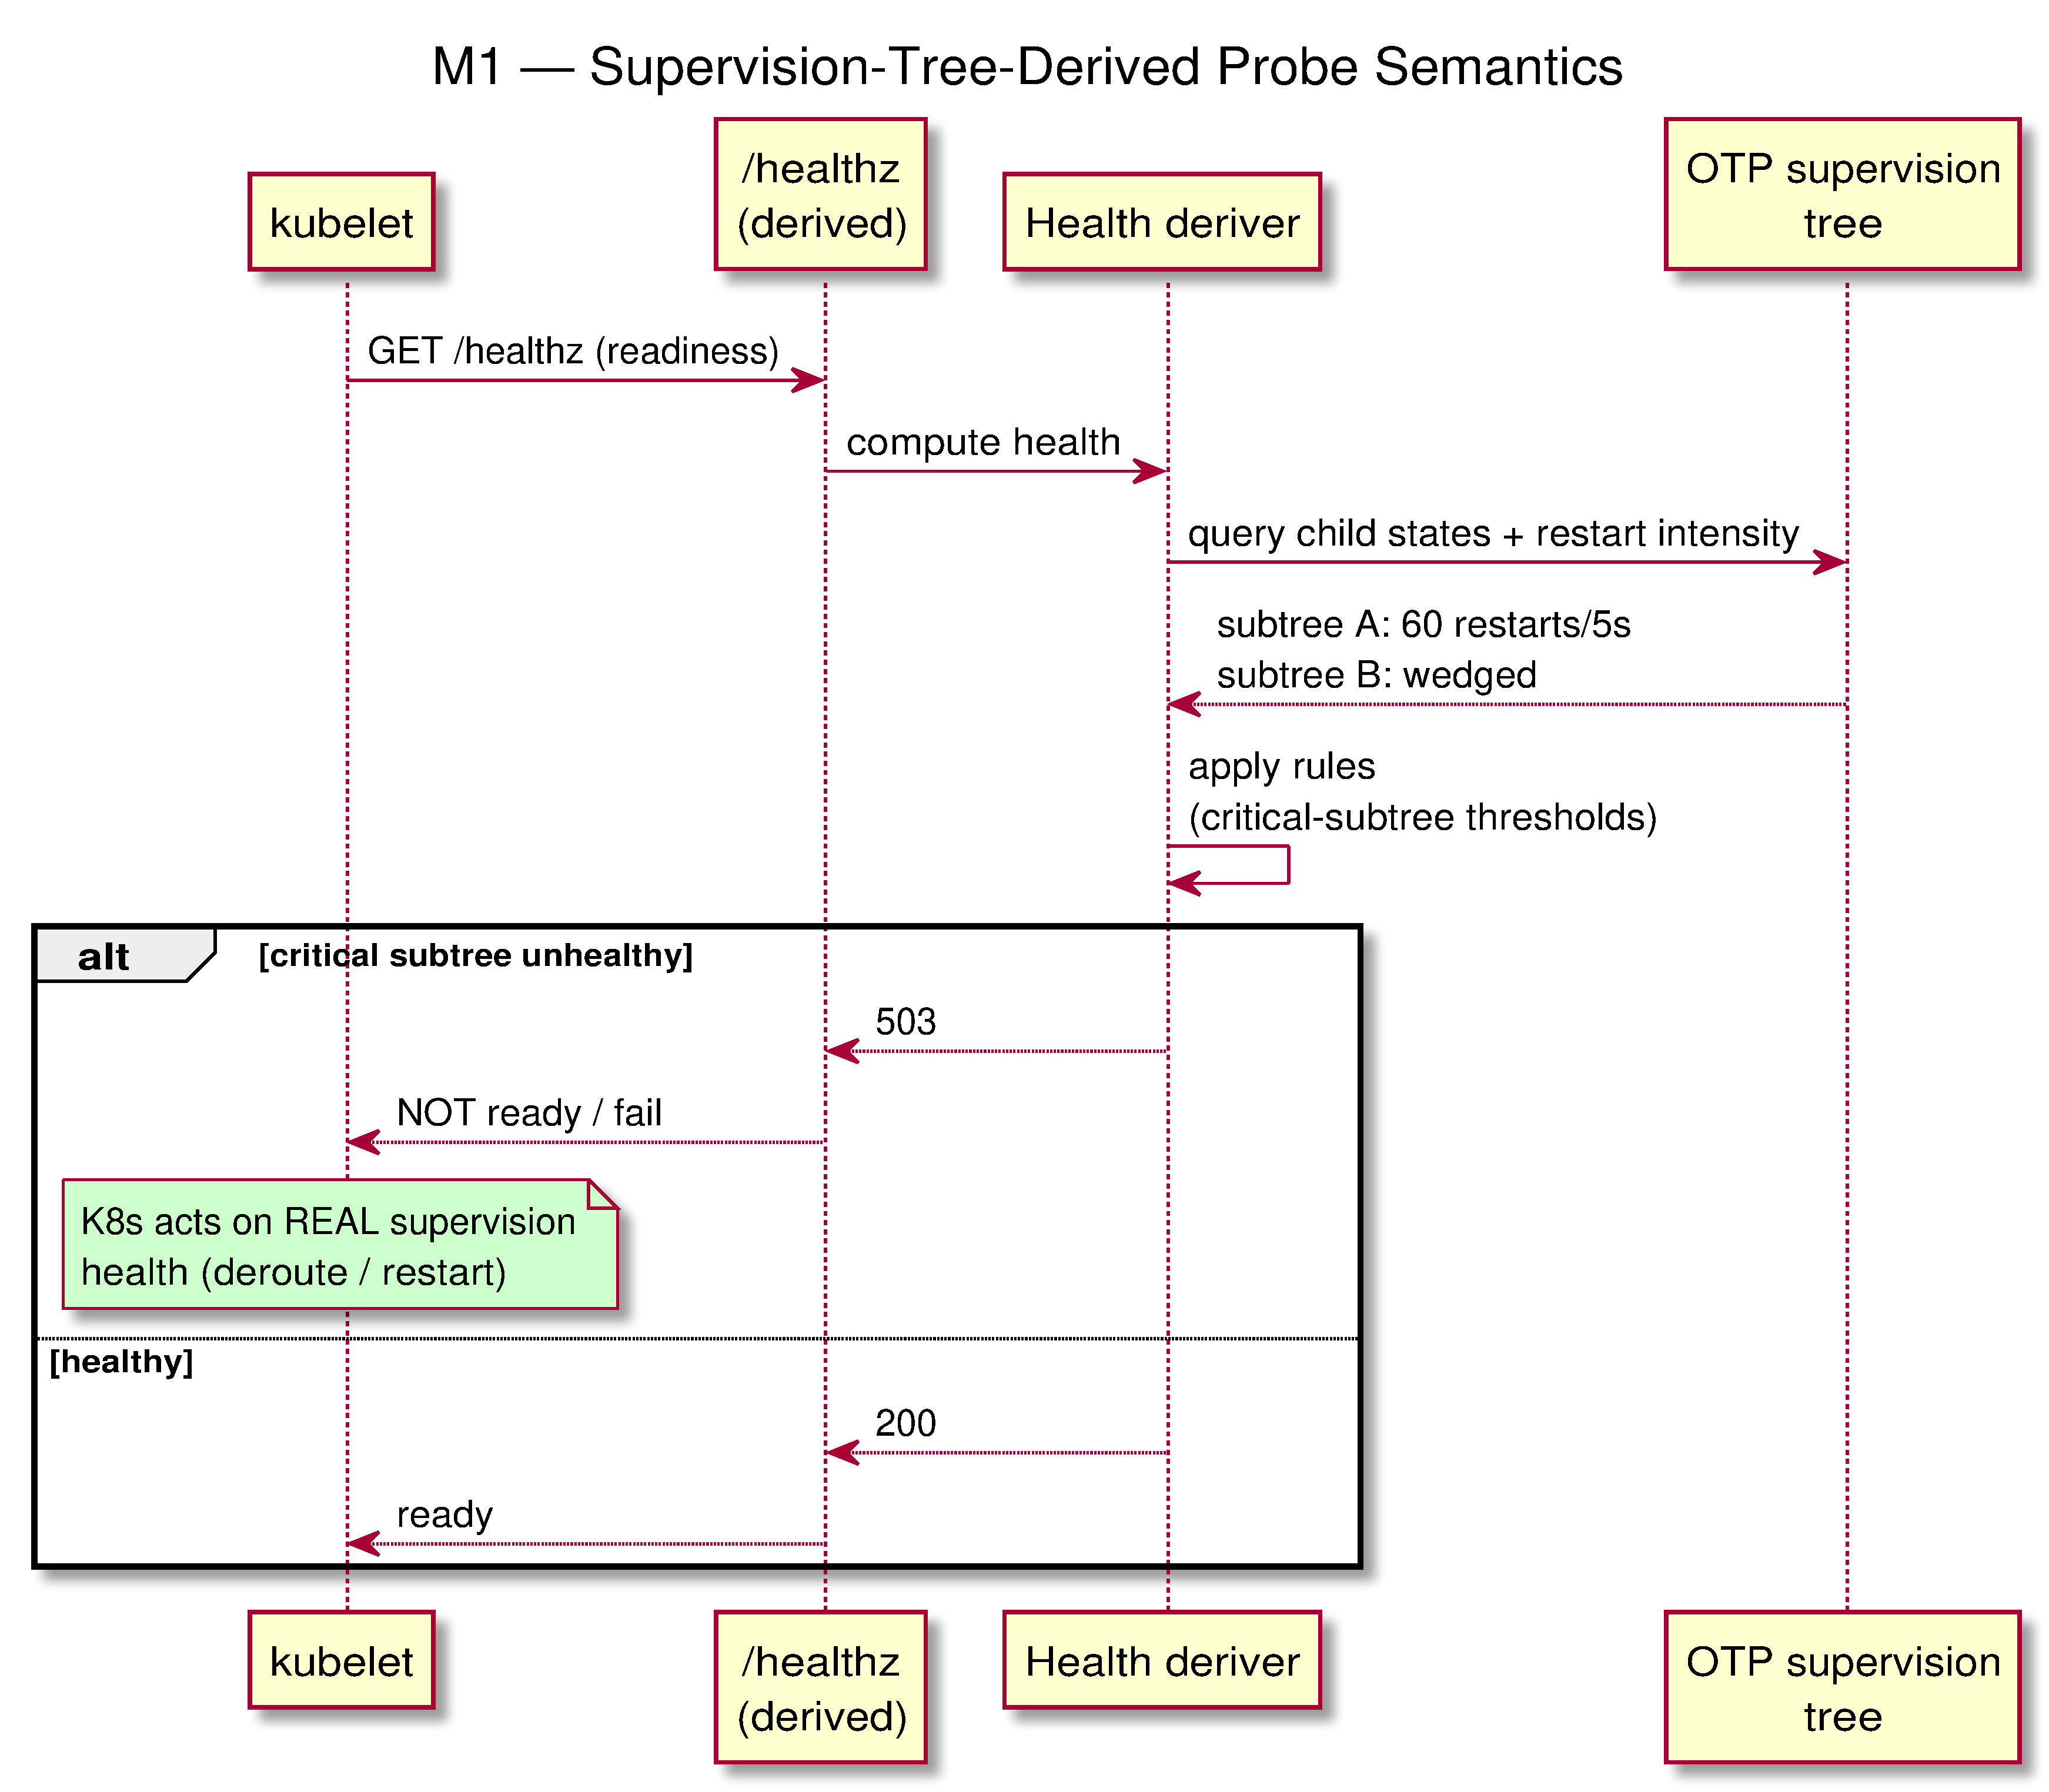
\includegraphics[width=\linewidth,height=0.9\textheight,keepaspectratio]{m1-supervision-derived-probes-sequence}
  \caption{M1 (sekuens): kubelet memanggil \texttt{/healthz}; \emph{health deriver} membaca
  keadaan \emph{supervision tree} dan membalas sehat/tidak berdasarkan intensitas
  \emph{restart} serta deteksi macet, bukan sekadar penerimaan \emph{socket}.}\label{fig:m1-seq}\end{figure}
\begin{figure}[H]\centering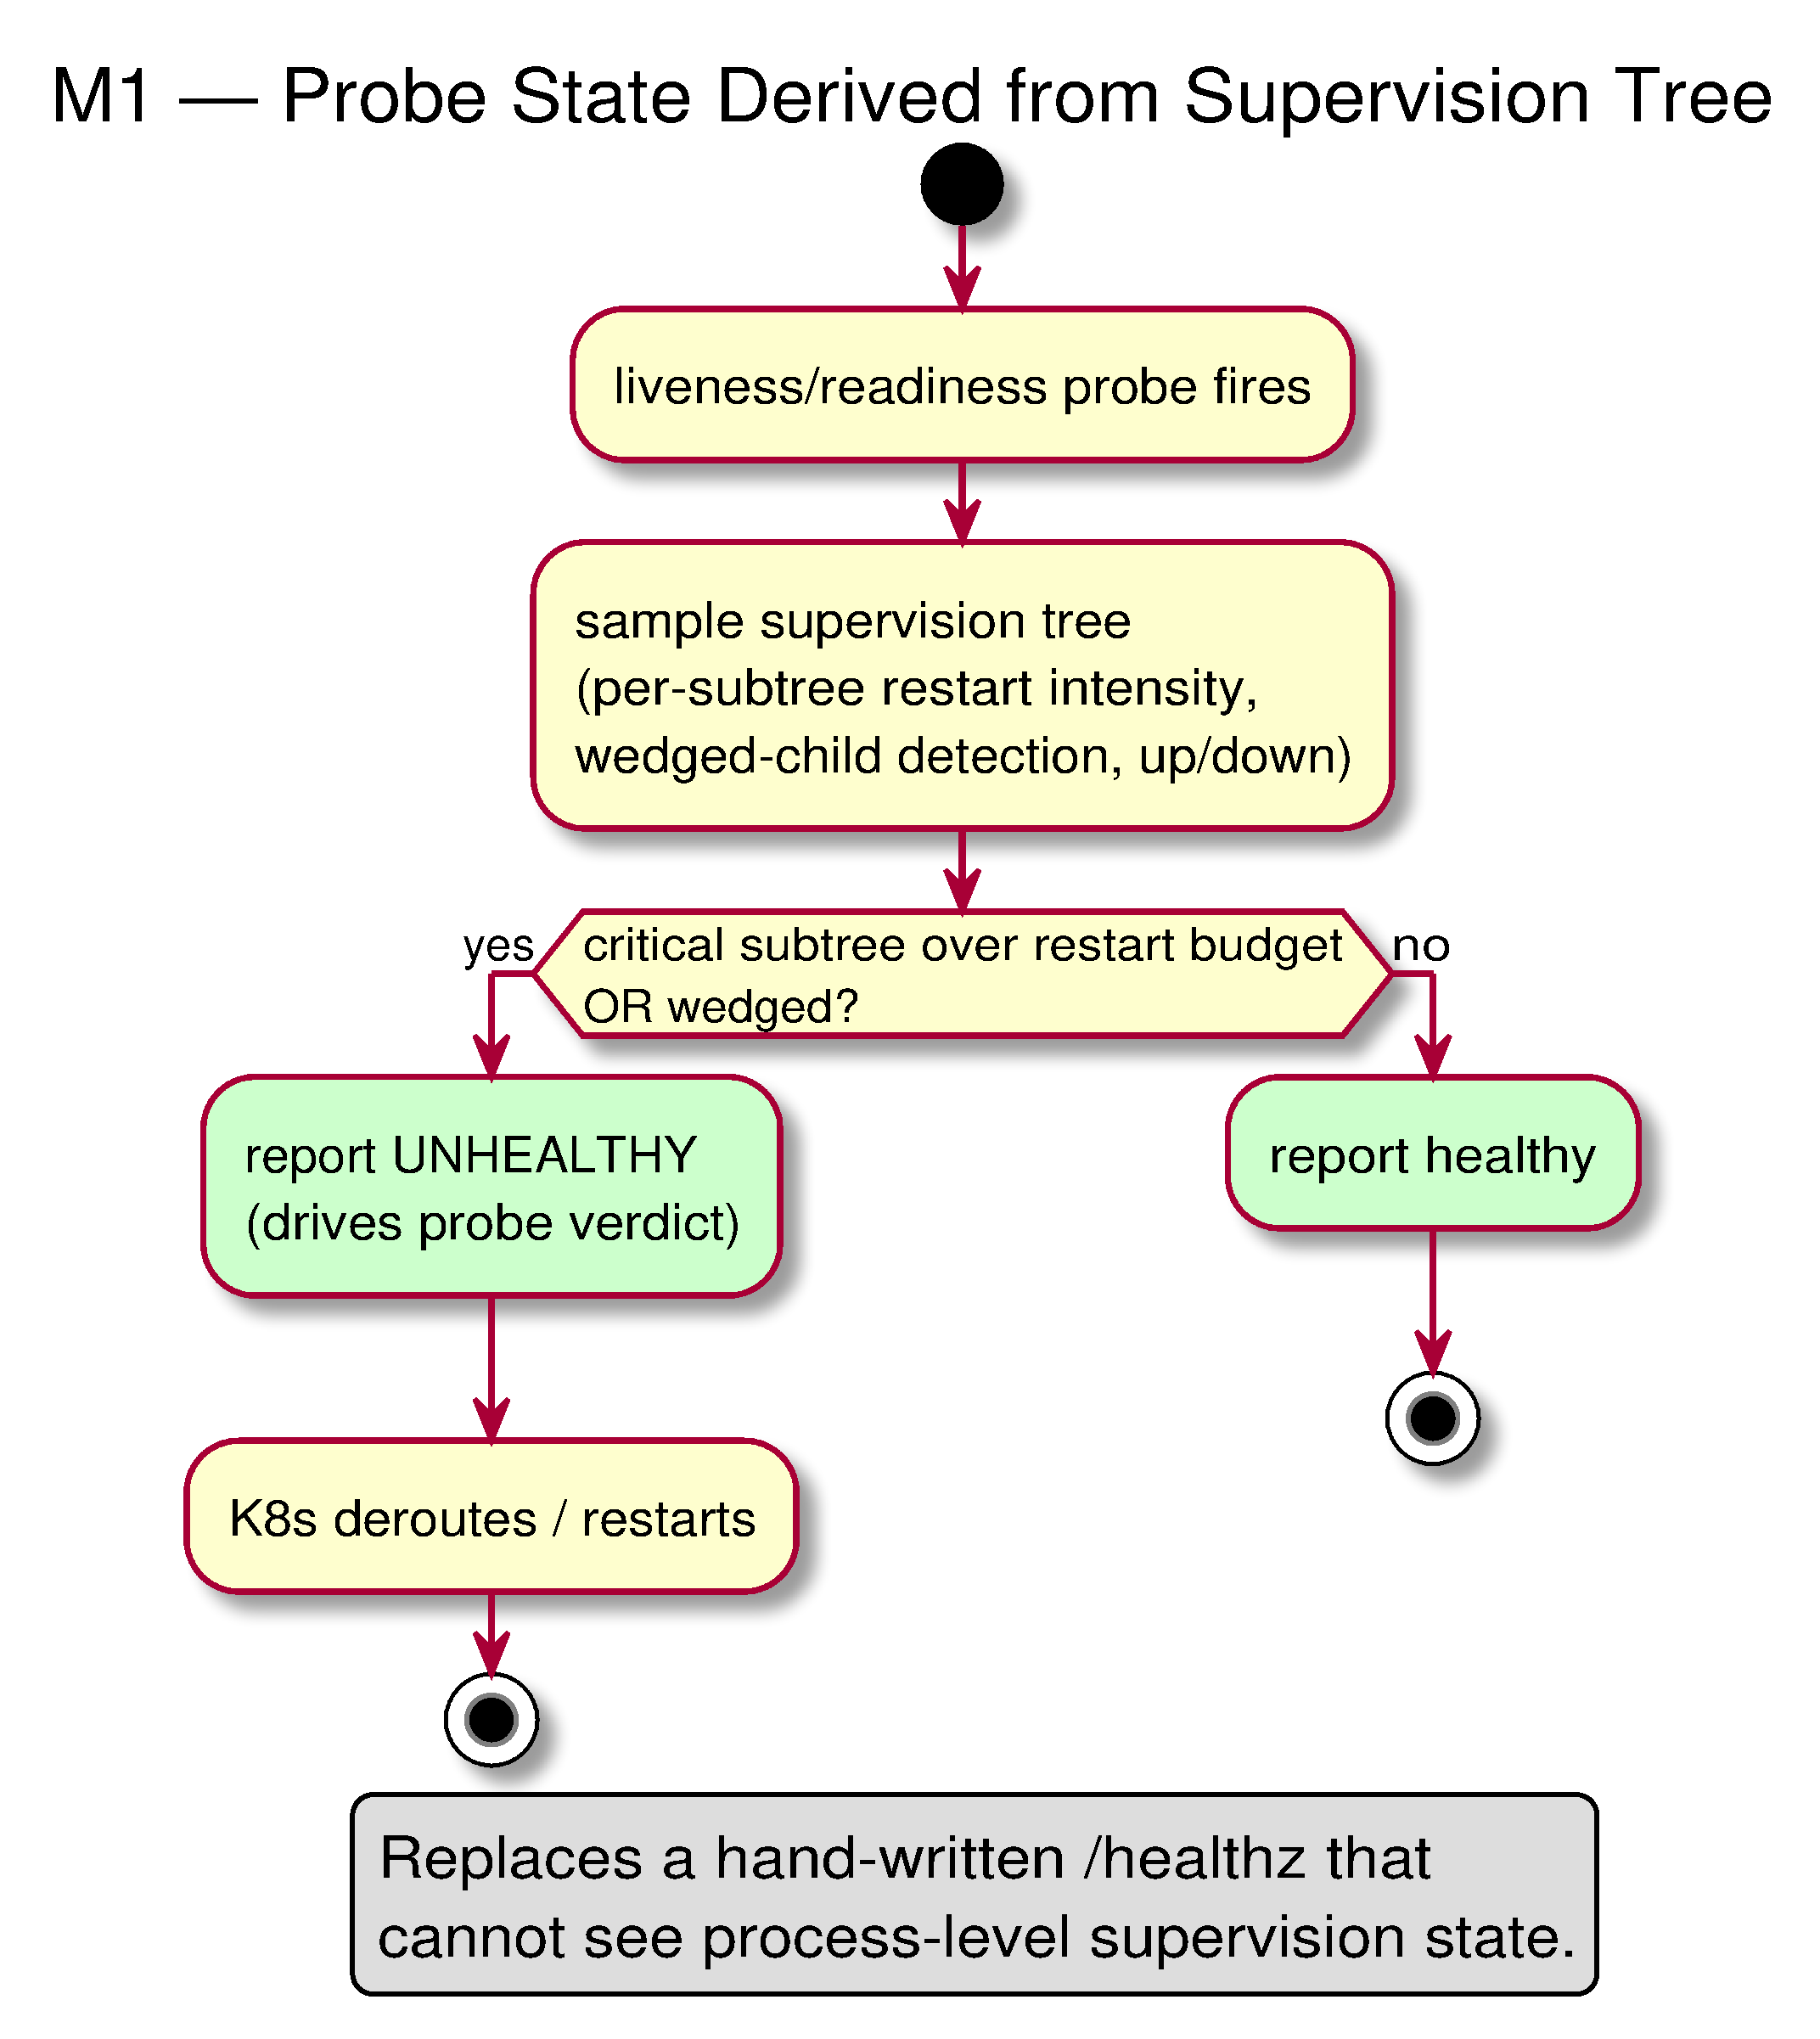
\includegraphics[width=\linewidth,height=0.9\textheight,keepaspectratio]{m1-supervision-derived-probes-activity}
  \caption{M1 (aktivitas): keputusan bercabang pada ``subpohon kritis macet atau
  over-\emph{restart}?''; bila ya, \emph{pod} dinyatakan tidak sehat sehingga Kubernetes
  men-\emph{deroute}/me-\emph{restart}.}\label{fig:m1-act}\end{figure}
\begin{algorithm}[H]\caption{M1 --- penurunan keadaan \emph{probe} dari \emph{supervision tree}.}\label{alg:m1}
\begin{algorithmic}[1]
\Function{ProbeHandler}{} \Comment{dipanggil saat /healthz}
  \State $S \gets$ \Call{InspectSupervisionTree}{} \Comment{intensitas restart, deteksi macet}
  \If{$\exists\, t \in S : t.\textit{restartRate} > \tau$ \textbf{ or } $t.\textit{wedged}$}
    \State \Return $503$ \Comment{tidak sehat}
  \Else
    \State \Return $200$
  \EndIf
\EndFunction
\end{algorithmic}\end{algorithm}

\noindent\textbf{Pembahasan.} Diagram sekuens (Gambar~\ref{fig:m1-seq}) menelusuri jalur
\emph{probe}: kubelet~$\rightarrow$~\texttt{/healthz}~$\rightarrow$~\emph{health
deriver}~$\rightarrow$~\emph{supervision tree}, lalu vonis dikembalikan ke kubelet---berbeda
dari jalur naif Masalah~1 yang berhenti di \emph{listener}. Diagram aktivitas
(Gambar~\ref{fig:m1-act}) menempatkan satu percabangan inti: bila ada subpohon kritis yang
macet atau melampaui ambang \emph{restart}, alur menuju ``tidak sehat'' (jalur hijau yang
membuat Kubernetes bertindak). Algoritma~\ref{alg:m1} memerincinya: baris~2 mengambil
keadaan \emph{supervision tree}; baris~3 mengevaluasi tiap subpohon $t$ terhadap ambang
$\tau$ dan bendera \textit{wedged}; bila terpenuhi, baris~4 mengembalikan \texttt{503},
selainnya baris~6 mengembalikan \texttt{200}---memetakan kesehatan supervisi langsung ke
semantik \emph{probe}.

\section{M2 --- Delegasi Kepemilikan Kegagalan}
\label{sec:m2}
Sebuah pengklasifikasi memutuskan lapis mana (supervisor OTP atau pengendali Kubernetes)
yang memulihkan suatu kelas kegagalan, sehingga menghindari pemulihan ganda.
\begin{figure}[H]\centering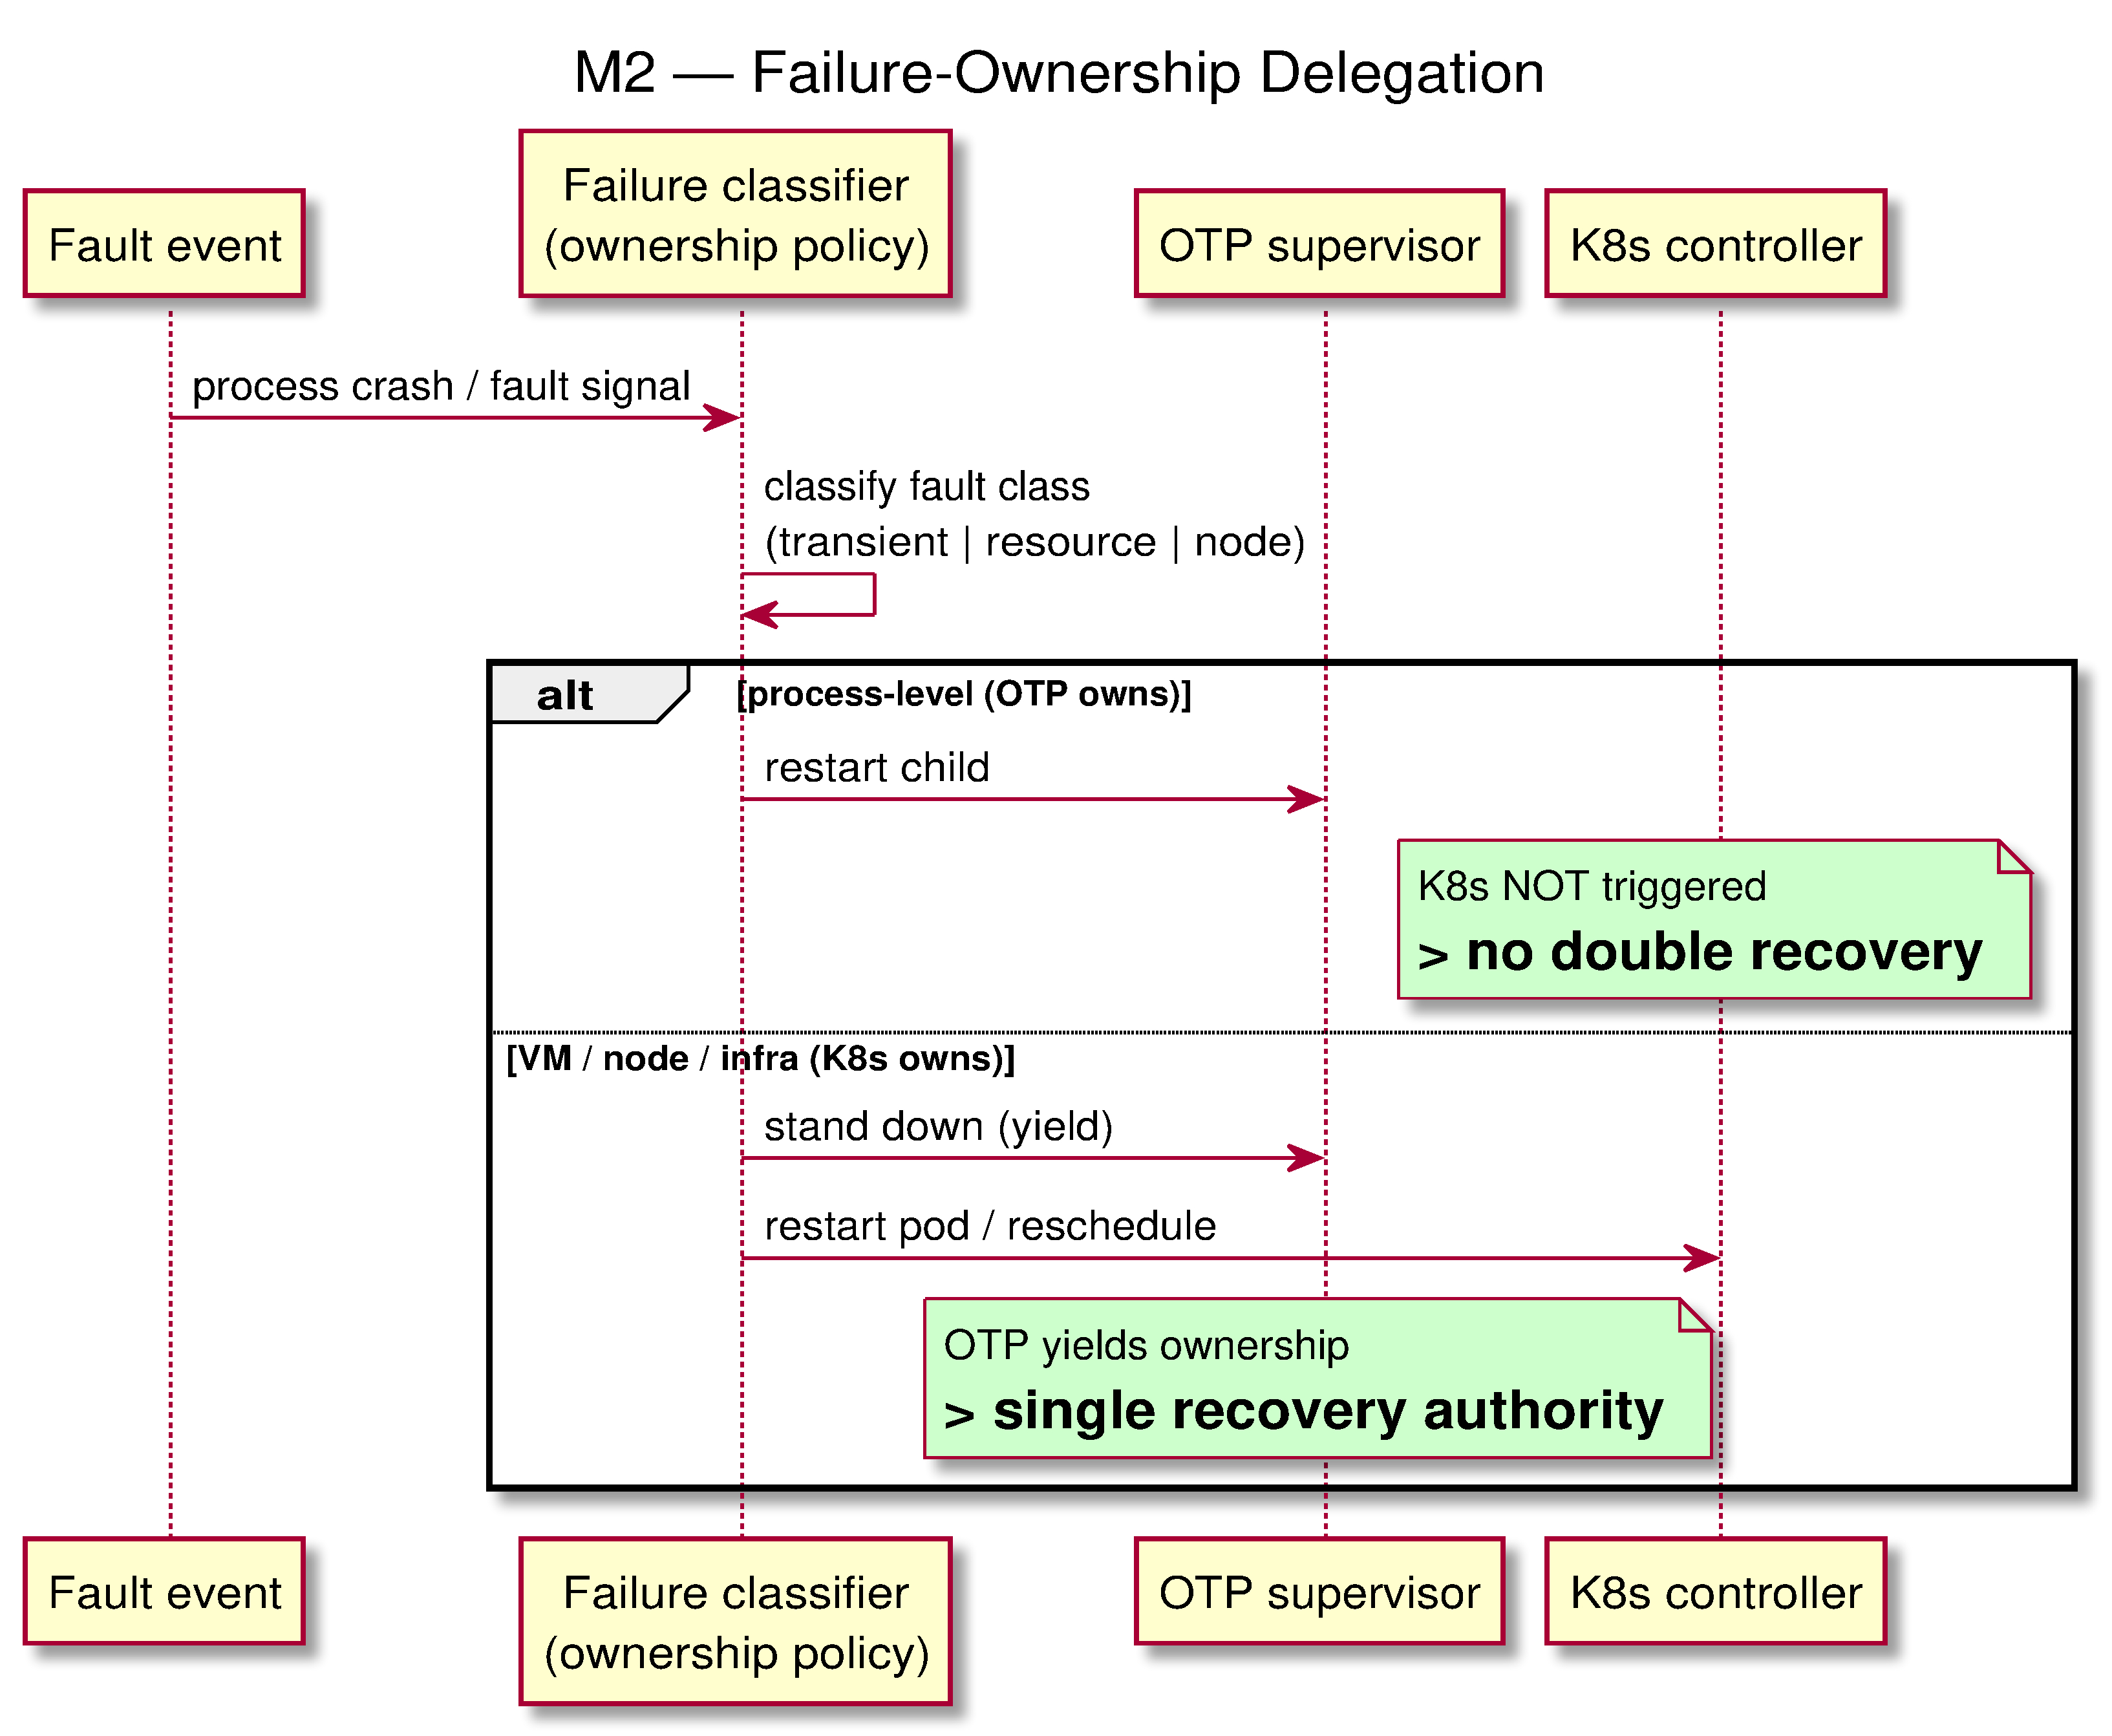
\includegraphics[width=\linewidth,height=0.9\textheight,keepaspectratio]{m2-failure-ownership-delegation-sequence}
  \caption{M2 (sekuens): \emph{fault event} masuk ke pengklasifikasi; berdasarkan kelasnya,
  hanya \emph{satu} otoritas (OTP \emph{atau} Kubernetes) yang dipicu.}\label{fig:m2-seq}\end{figure}
\begin{figure}[H]\centering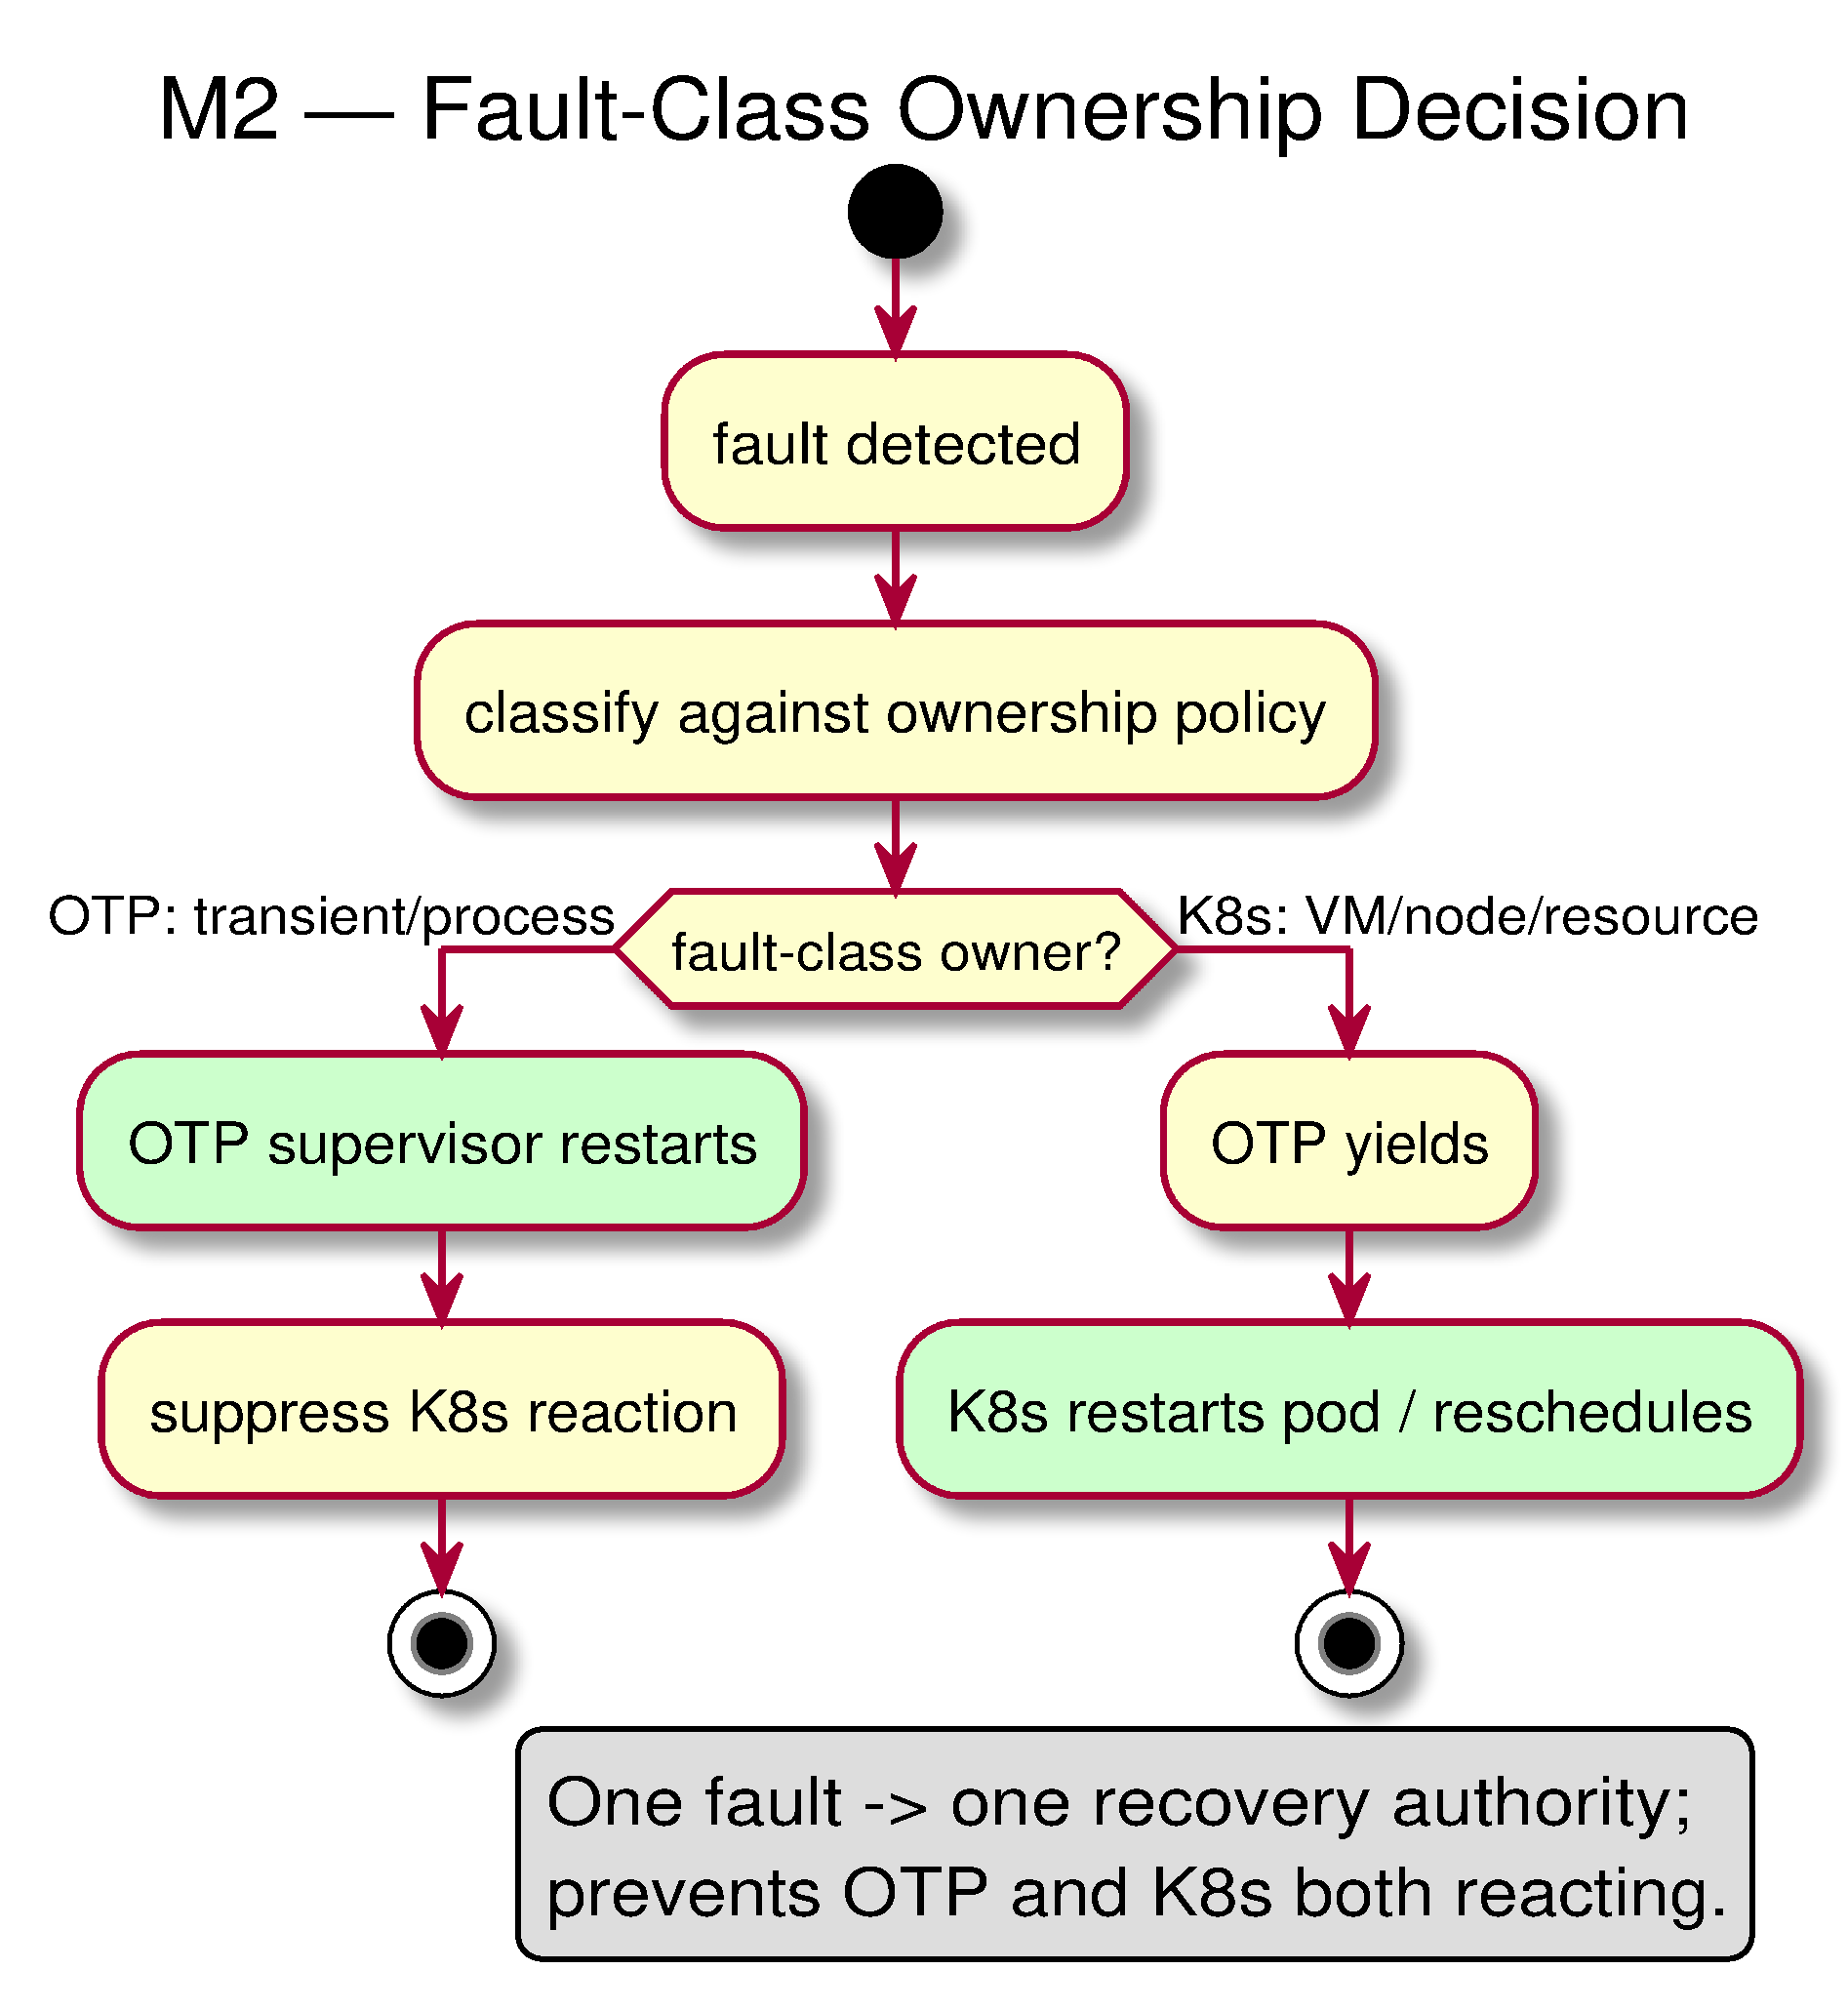
\includegraphics[width=\linewidth,height=0.9\textheight,keepaspectratio]{m2-failure-ownership-delegation-activity}
  \caption{M2 (aktivitas): keputusan kepemilikan menurut kelas kegagalan
  (proses/sumber daya/node), memetakan tiap kelas ke tepat satu lapis pemulihan.}\label{fig:m2-act}\end{figure}
\begin{algorithm}[H]\caption{M2 --- delegasi kepemilikan kegagalan.}\label{alg:m2}
\begin{algorithmic}[1]
\Procedure{OnFault}{$f$}
  \State $c \gets$ \Call{Classify}{$f$} \Comment{transient $\mid$ resource $\mid$ node}
  \If{$c = \textit{process}$}
    \State \Call{OTP.Restart}{$f.\textit{child}$} \Comment{K8s tidak diberi tahu}
  \Else
    \State \Call{OTP.StandDown}{$f$}; \Call{K8s.RestartPod}{}
  \EndIf
\EndProcedure
\end{algorithmic}\end{algorithm}

\noindent\textbf{Pembahasan.} Diagram sekuens (Gambar~\ref{fig:m2-seq}) menunjukkan
\emph{fault event}~$\rightarrow$~\emph{failure classifier} yang lalu mengarahkan pesan
\emph{hanya} ke satu otoritas, kebalikan dari Masalah~2 yang kedua lapisnya bereaksi.
Diagram aktivitas (Gambar~\ref{fig:m2-act}) adalah pohon keputusan berlabel kelas
kegagalan. Algoritma~\ref{alg:m2} memformalkannya: baris~2 mengklasifikasi $f$; bila
kelasnya \textit{process} (baris~3), baris~4 me-\emph{restart} via OTP \emph{tanpa}
memberi tahu Kubernetes; selainnya baris~6 membuat OTP mundur dan menyerahkan pemulihan
ke Kubernetes---kontrak ``satu kegagalan, satu otoritas''.

\section{M3 --- Pengendali Umpan-Balik: \emph{Grace} $\leftrightarrow$ Konvergensi $\leftrightarrow$ \emph{Probe}}
\label{sec:m3}
Sebuah pengendali menghitung \texttt{terminationGracePeriodSeconds} secara dinamis dari
\emph{backlog} \emph{handoff} Horde dan waktu konvergensi libcluster, sehingga \emph{drain}
dan \emph{handoff} selesai sebelum \texttt{SIGKILL}.
\begin{figure}[H]\centering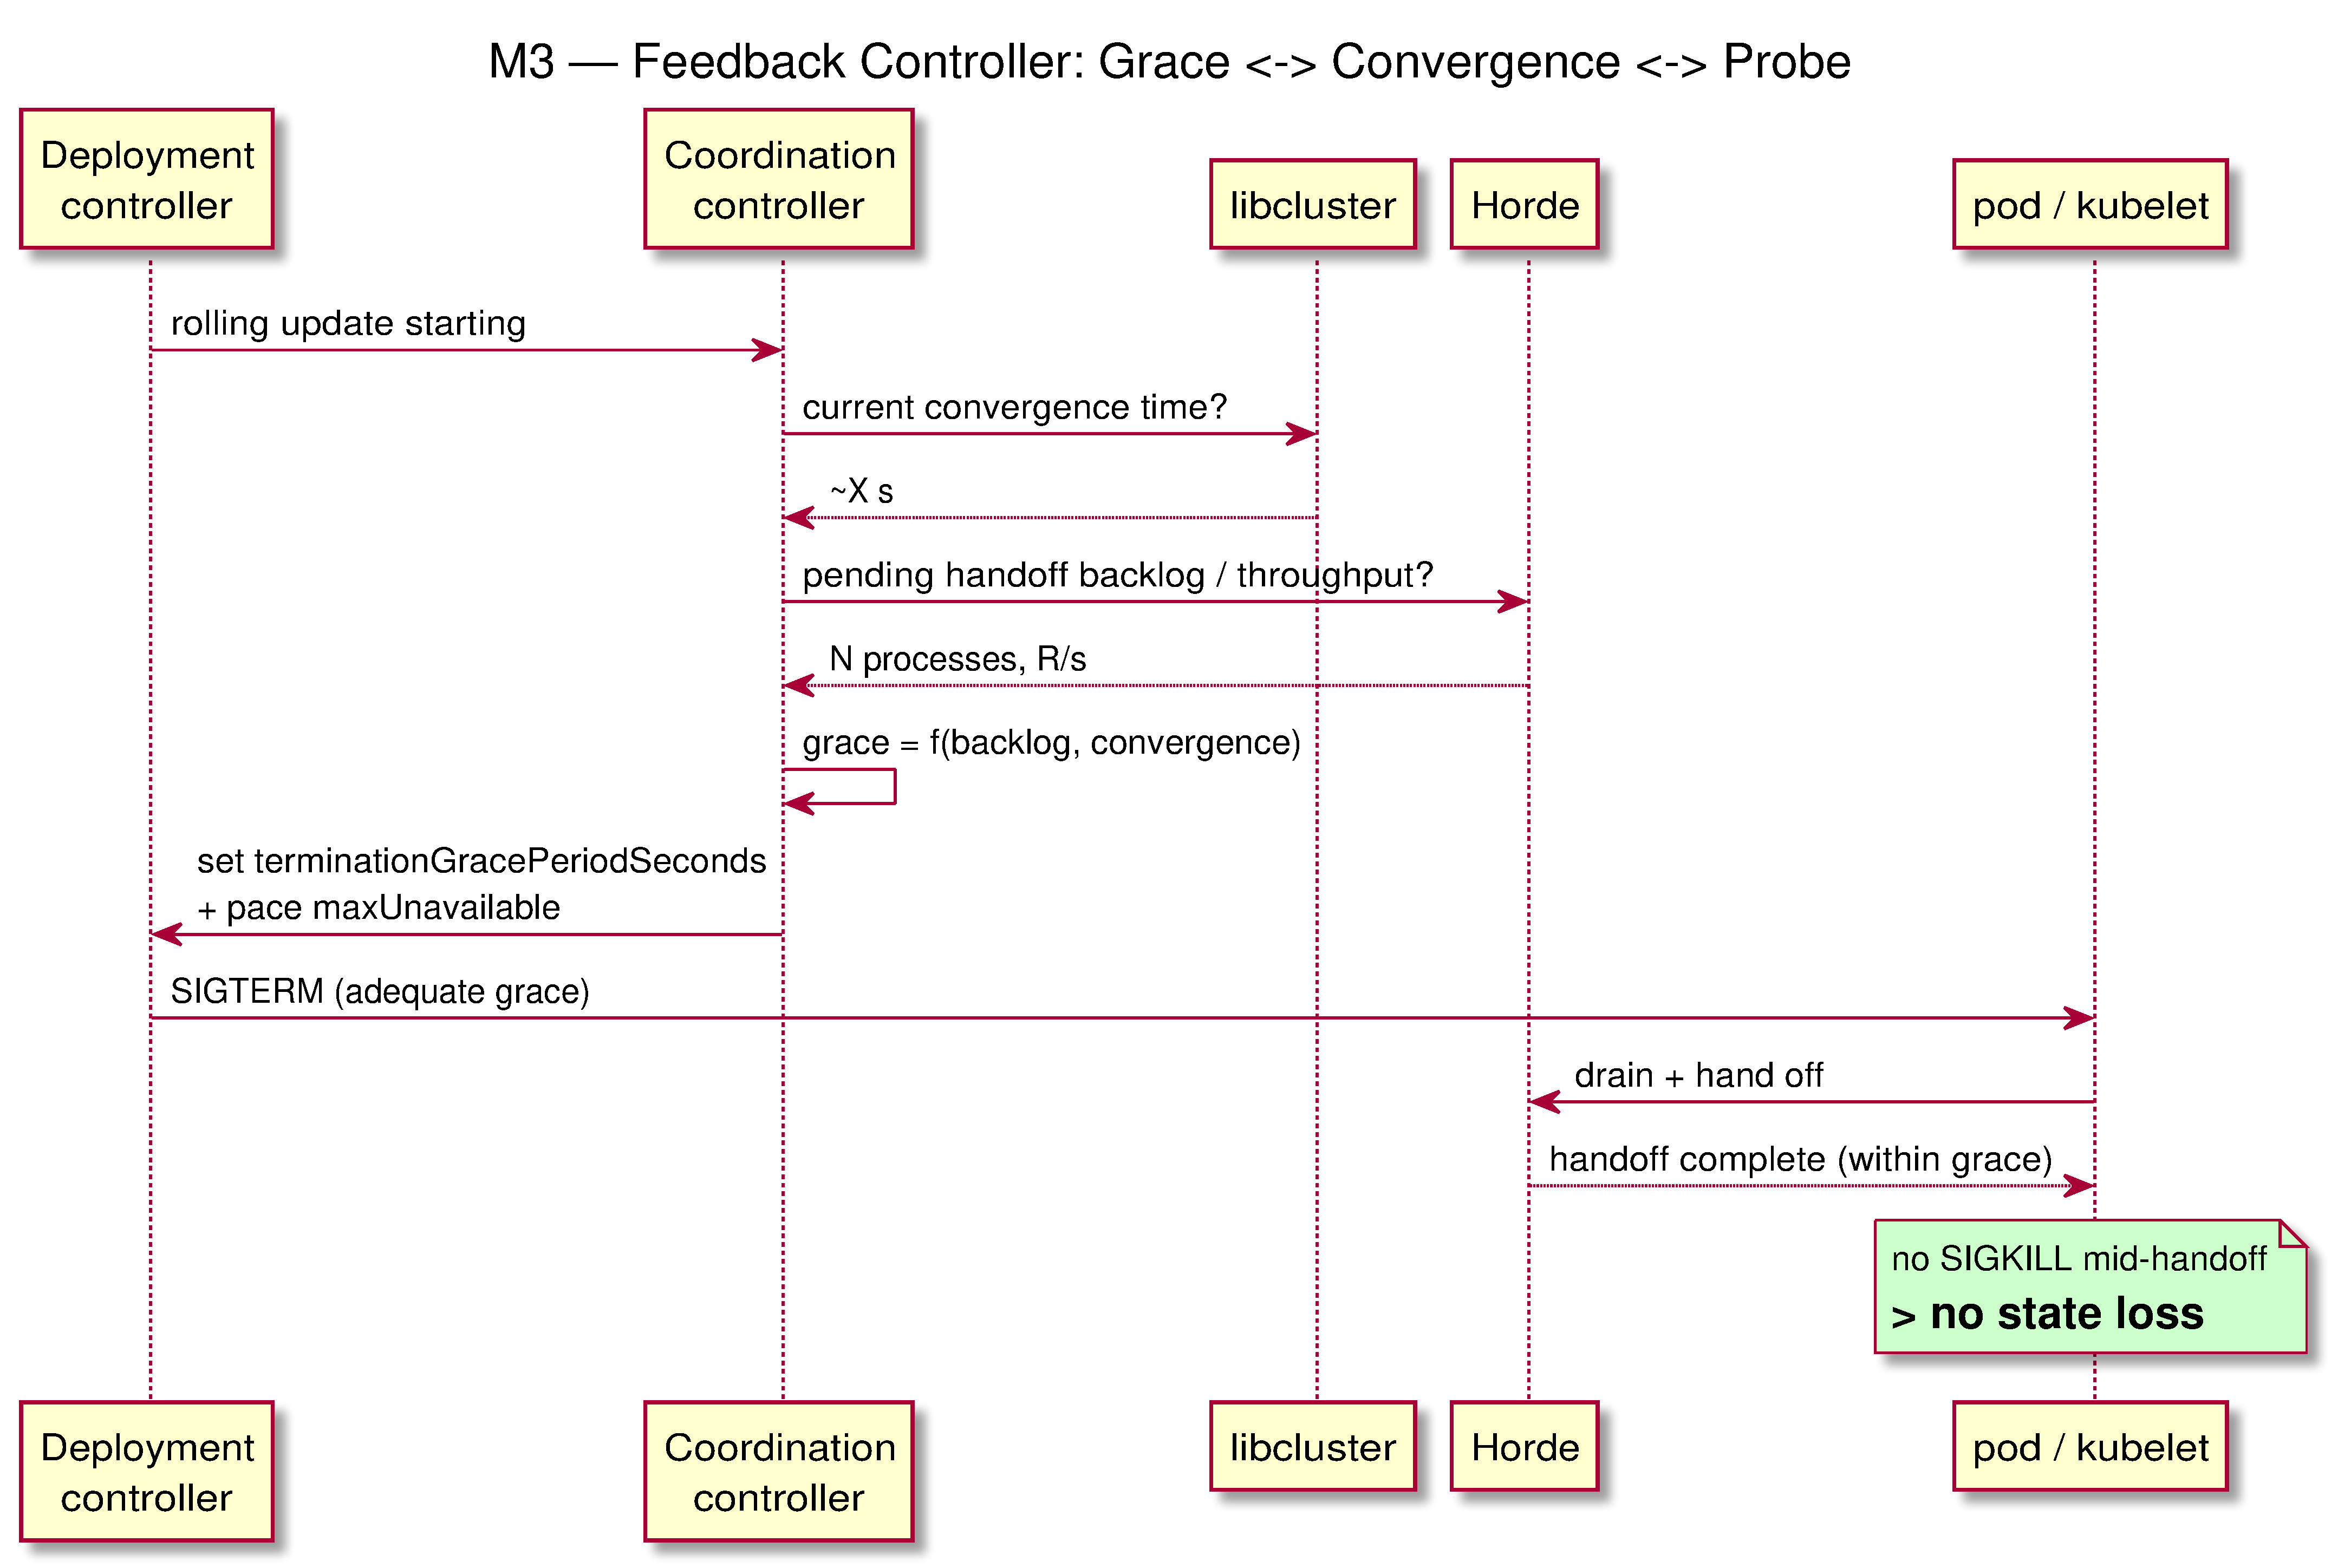
\includegraphics[width=\linewidth,height=0.9\textheight,keepaspectratio]{m3-grace-convergence-controller-sequence}
  \caption{M3 (sekuens): pengendali koordinasi mengukur \emph{backlog}/laju \emph{handoff}
  dan waktu konvergensi, lalu menetapkan \emph{grace period} yang memadai sebelum
  \texttt{SIGTERM} dikirim.}\label{fig:m3-seq}\end{figure}
\begin{figure}[H]\centering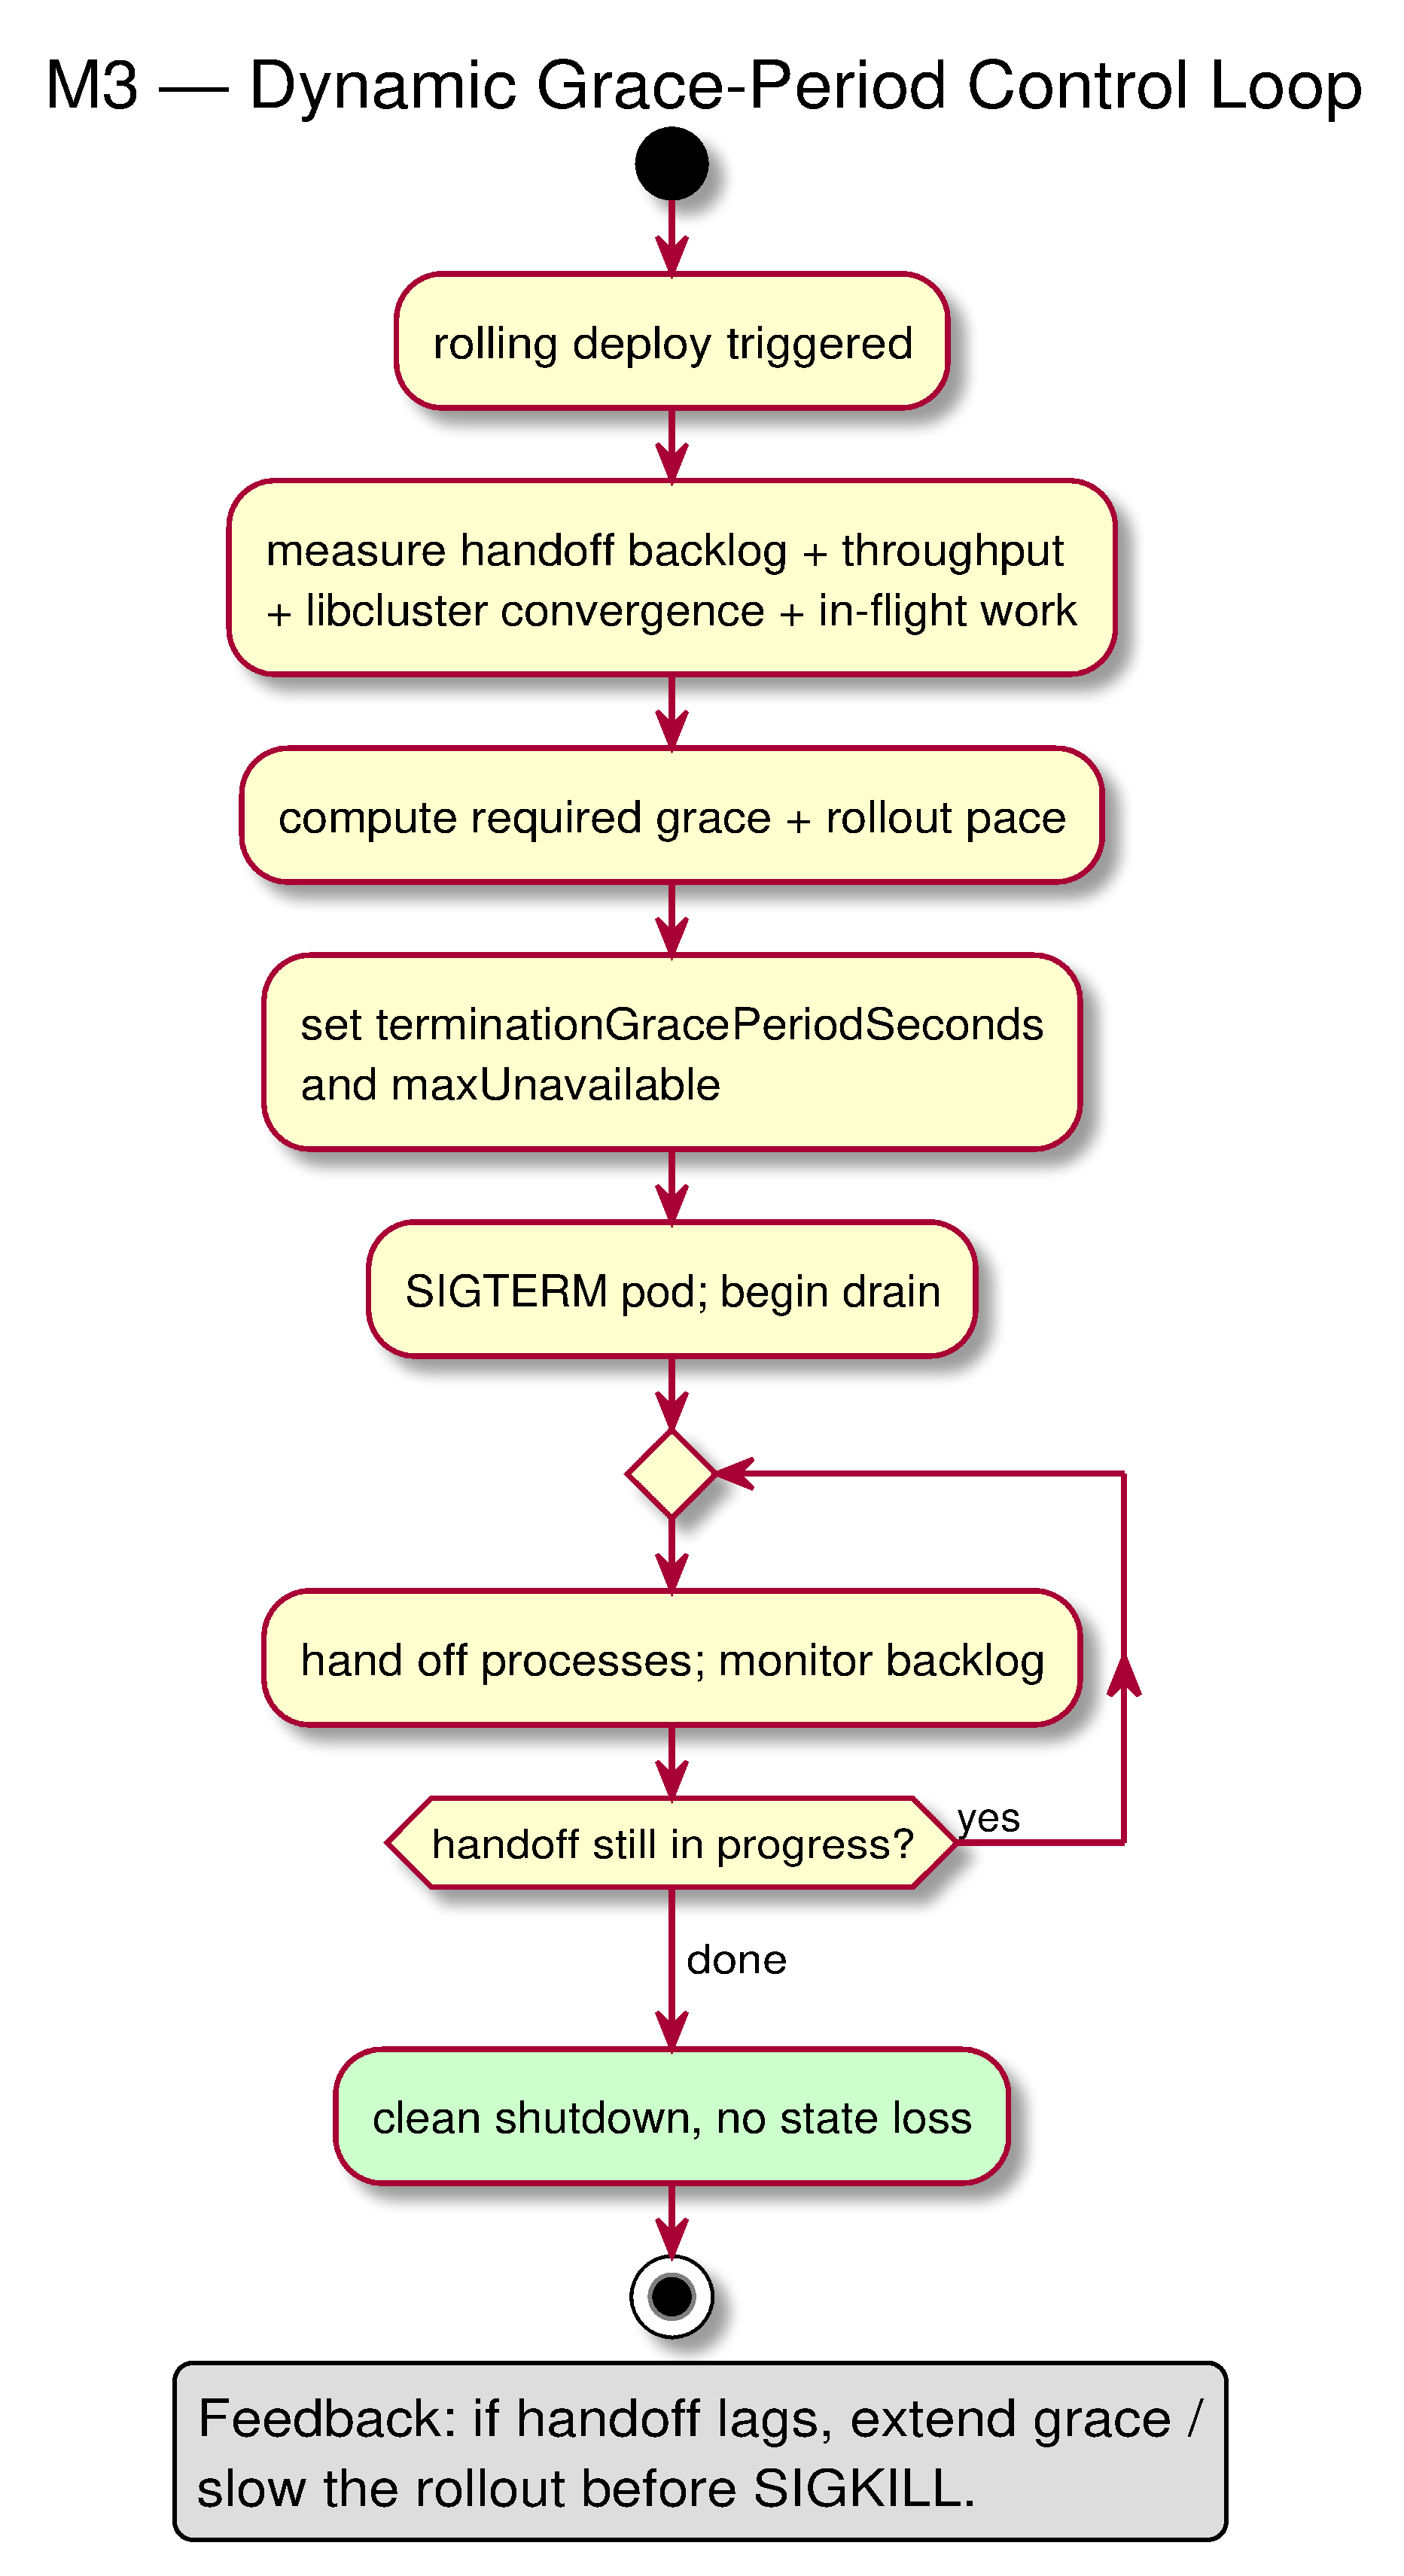
\includegraphics[width=\linewidth,height=0.9\textheight,keepaspectratio]{m3-grace-convergence-controller-activity}
  \caption{M3 (aktivitas): \emph{loop} kendali yang memperpanjang \emph{grace}/memperlambat
  \emph{rollout} bila \emph{handoff} melambat, hingga \emph{handoff} tuntas.}\label{fig:m3-act}\end{figure}
\begin{algorithm}[H]\caption{M3 --- kendali \emph{grace period} dinamis.}\label{alg:m3}
\begin{algorithmic}[1]
\Procedure{OnRollingUpdate}{}
  \State $g \gets \max(\textsc{HandoffBacklog}()/\rho,\ \textsc{ConvergenceTime}(),\ g_{\min})$
  \State \Call{SetGracePeriod}{$g$}; \Call{Pace}{\textit{maxUnavailable}}
  \State \textbf{on} \texttt{SIGTERM}: \Call{Drain}{}
  \While{\Call{HandoffPending}{}}
    \State \Call{Handoff}{} \Comment{perpanjang $g$ bila melambat}
  \EndWhile
\EndProcedure
\end{algorithmic}\end{algorithm}

\noindent\textbf{Pembahasan.} Diagram sekuens (Gambar~\ref{fig:m3-seq}) menelusuri
pertanyaan pengendali ke libcluster (waktu konvergensi) dan Horde (\emph{backlog}/laju),
lalu penetapan \emph{grace} ke \emph{Deployment} sebelum \texttt{SIGTERM}---menutup celah
waktu Masalah~4. Diagram aktivitas (Gambar~\ref{fig:m3-act}) memodelkan \emph{loop} dengan
umpan balik: selama \emph{handoff} berjalan, \emph{grace} diperpanjang/rollout diperlambat.
Algoritma~\ref{alg:m3} memerincinya: baris~2 menghitung \emph{grace} $g$ sebagai
\emph{maksimum} dari (waktu menghabiskan \emph{backlog} pada laju $\rho$, waktu
konvergensi, dan batas bawah $g_{\min}$); baris~3 menetapkan \emph{grace} dan men-\emph{pace}
\texttt{maxUnavailable}; baris~4 men-\emph{drain} saat \texttt{SIGTERM}; perulangan
baris~5--7 melanjutkan \emph{handoff} hingga tuntas.

\section{M4 --- \emph{Operator} Sadar-\emph{Cluster} BEAM + Jembatan Kesehatan}
\label{sec:m4}
Sebuah \emph{operator} (pengendali kustom Kubernetes, di sini ditulis dalam Elixir dengan
Bonny) memantulkan keanggotaan Horde/distribusi Erlang ke \emph{readiness} \emph{pod} dan
menahan terminasi hingga \emph{handoff} selesai. Jembatan
keanggotaan$\rightarrow$\emph{readiness} sudah ada di Akka; yang baru bagi BEAM adalah
penahanan terminasi dan kesadaran \emph{supervision tree}.
\begin{figure}[H]\centering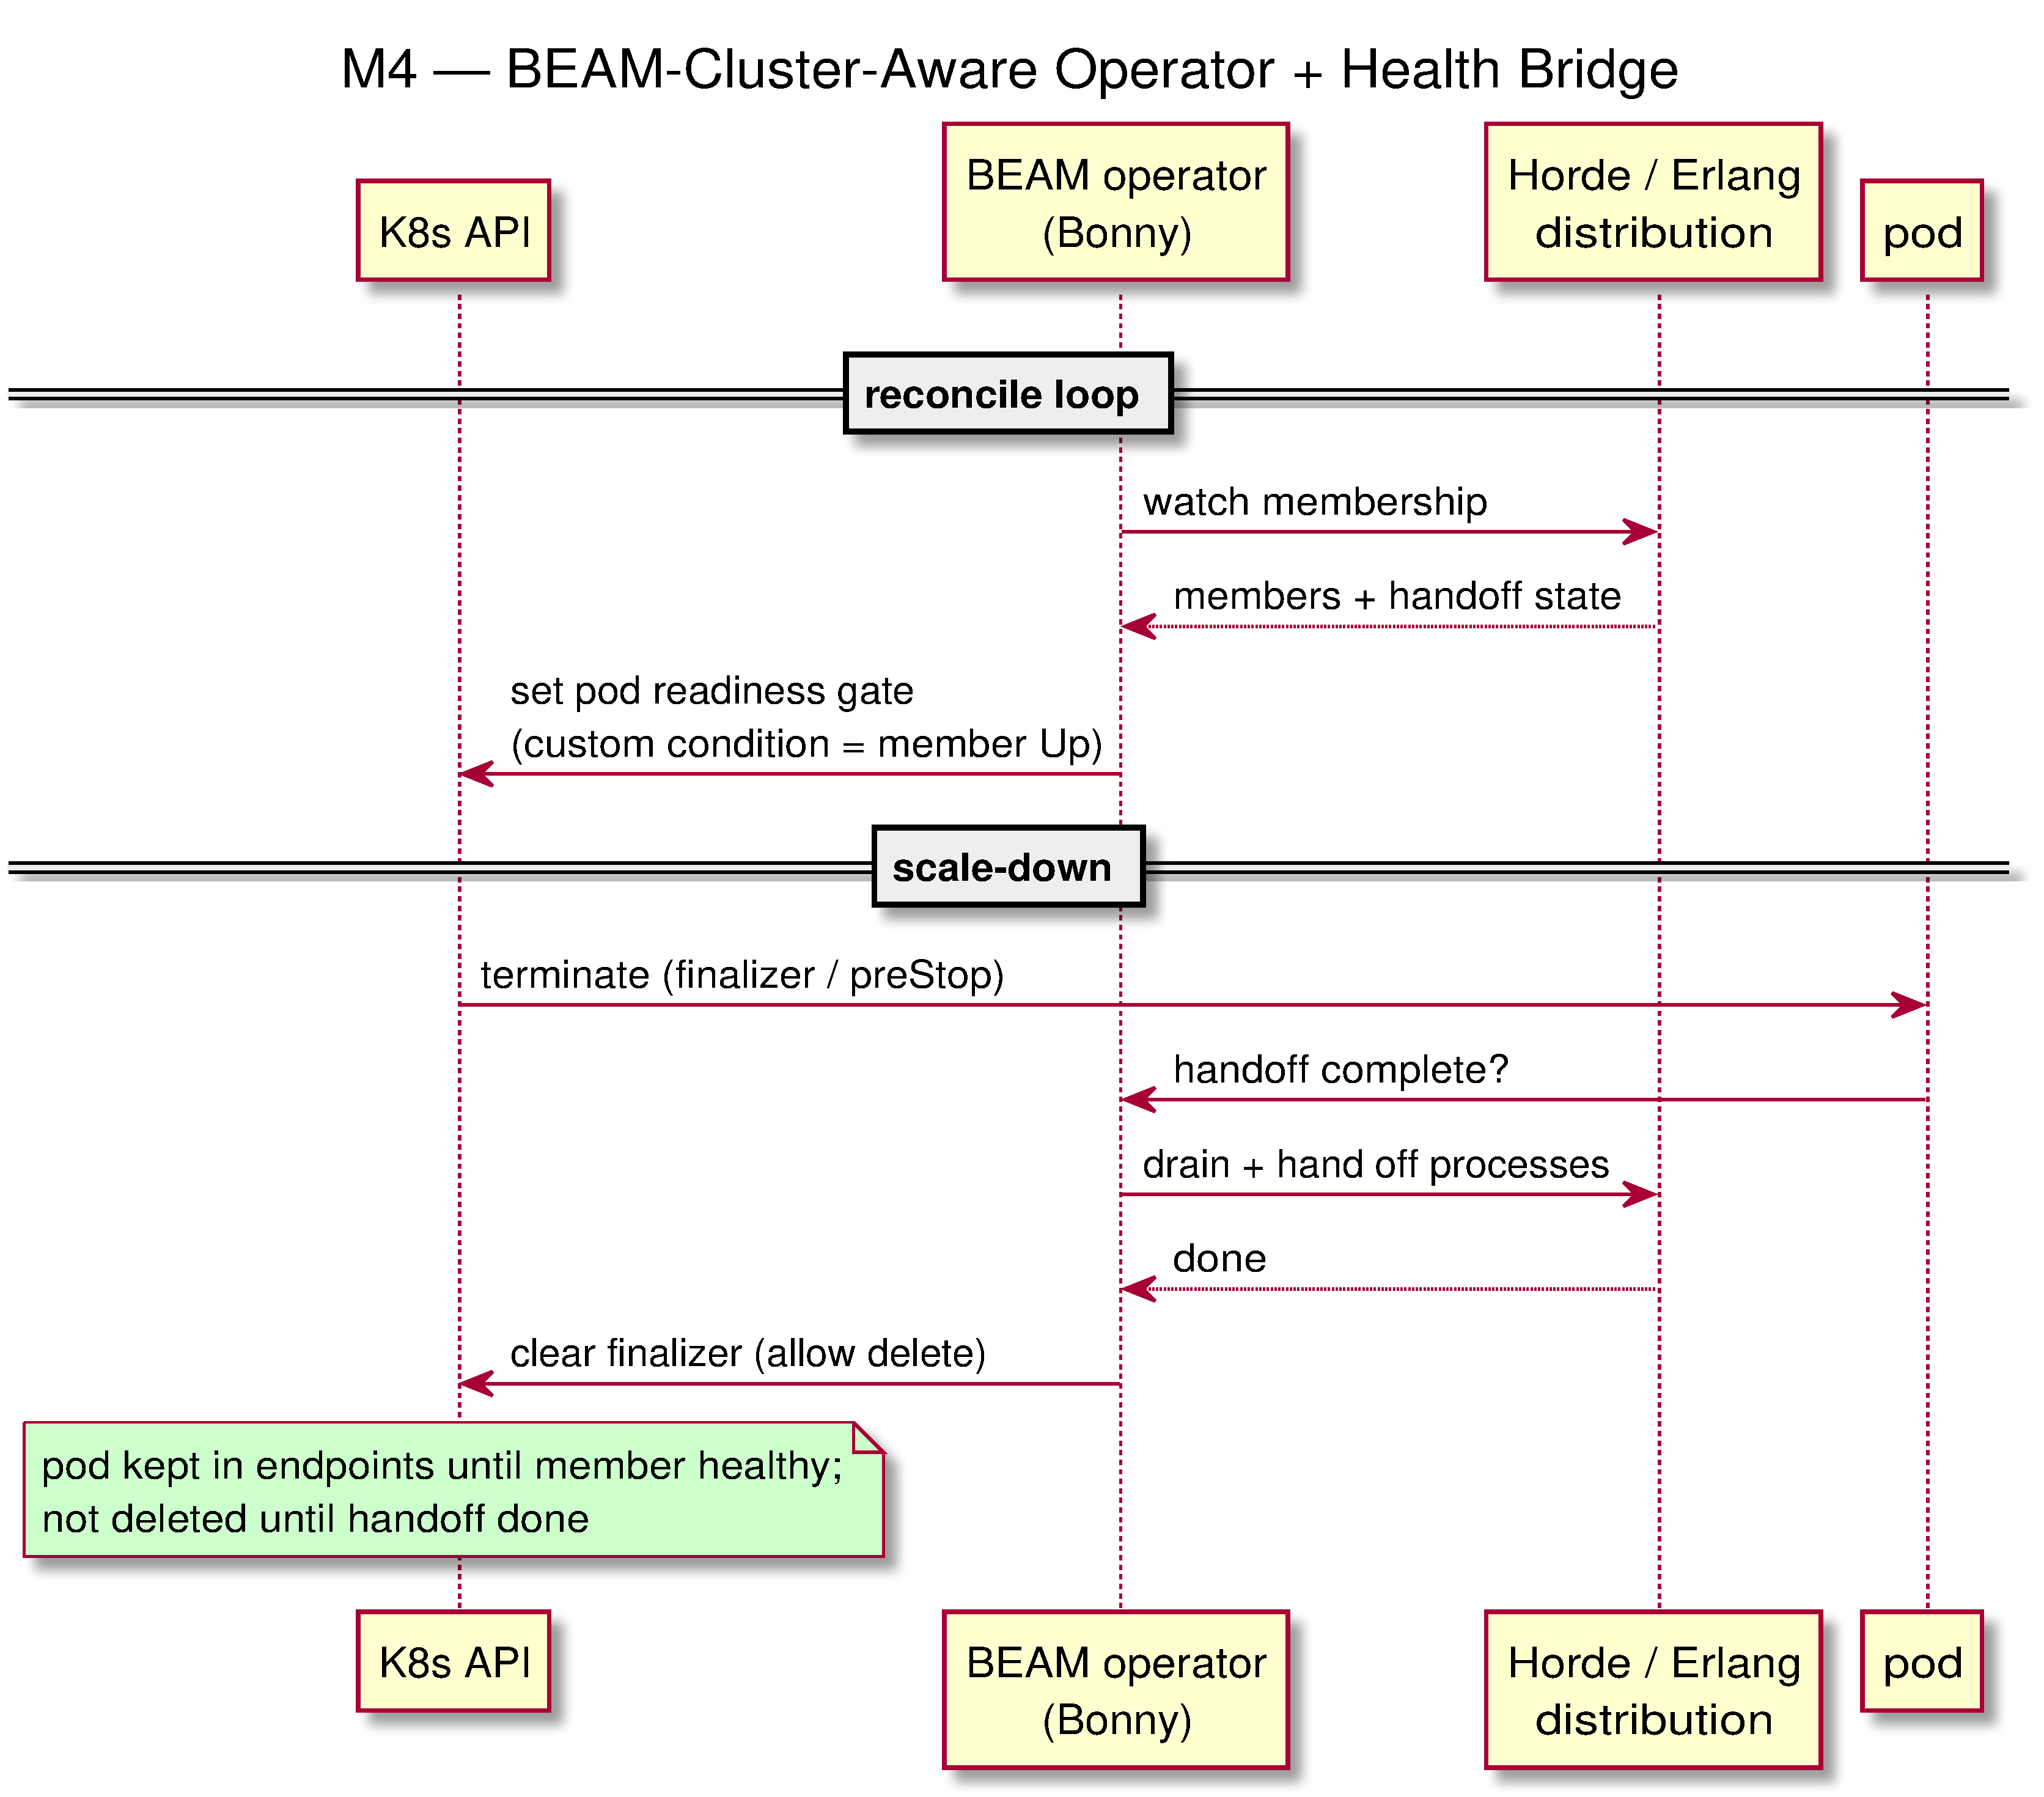
\includegraphics[width=\linewidth,height=0.9\textheight,keepaspectratio]{m4-cluster-aware-operator-sequence}
  \caption{M4 (sekuens): operator mengawasi keanggotaan dan menyetel \emph{readiness gate};
  saat terminasi, ia menahan via \emph{finalizer} sampai \emph{handoff} selesai sebelum
  melepas \emph{pod}.}\label{fig:m4-seq}\end{figure}
\begin{figure}[H]\centering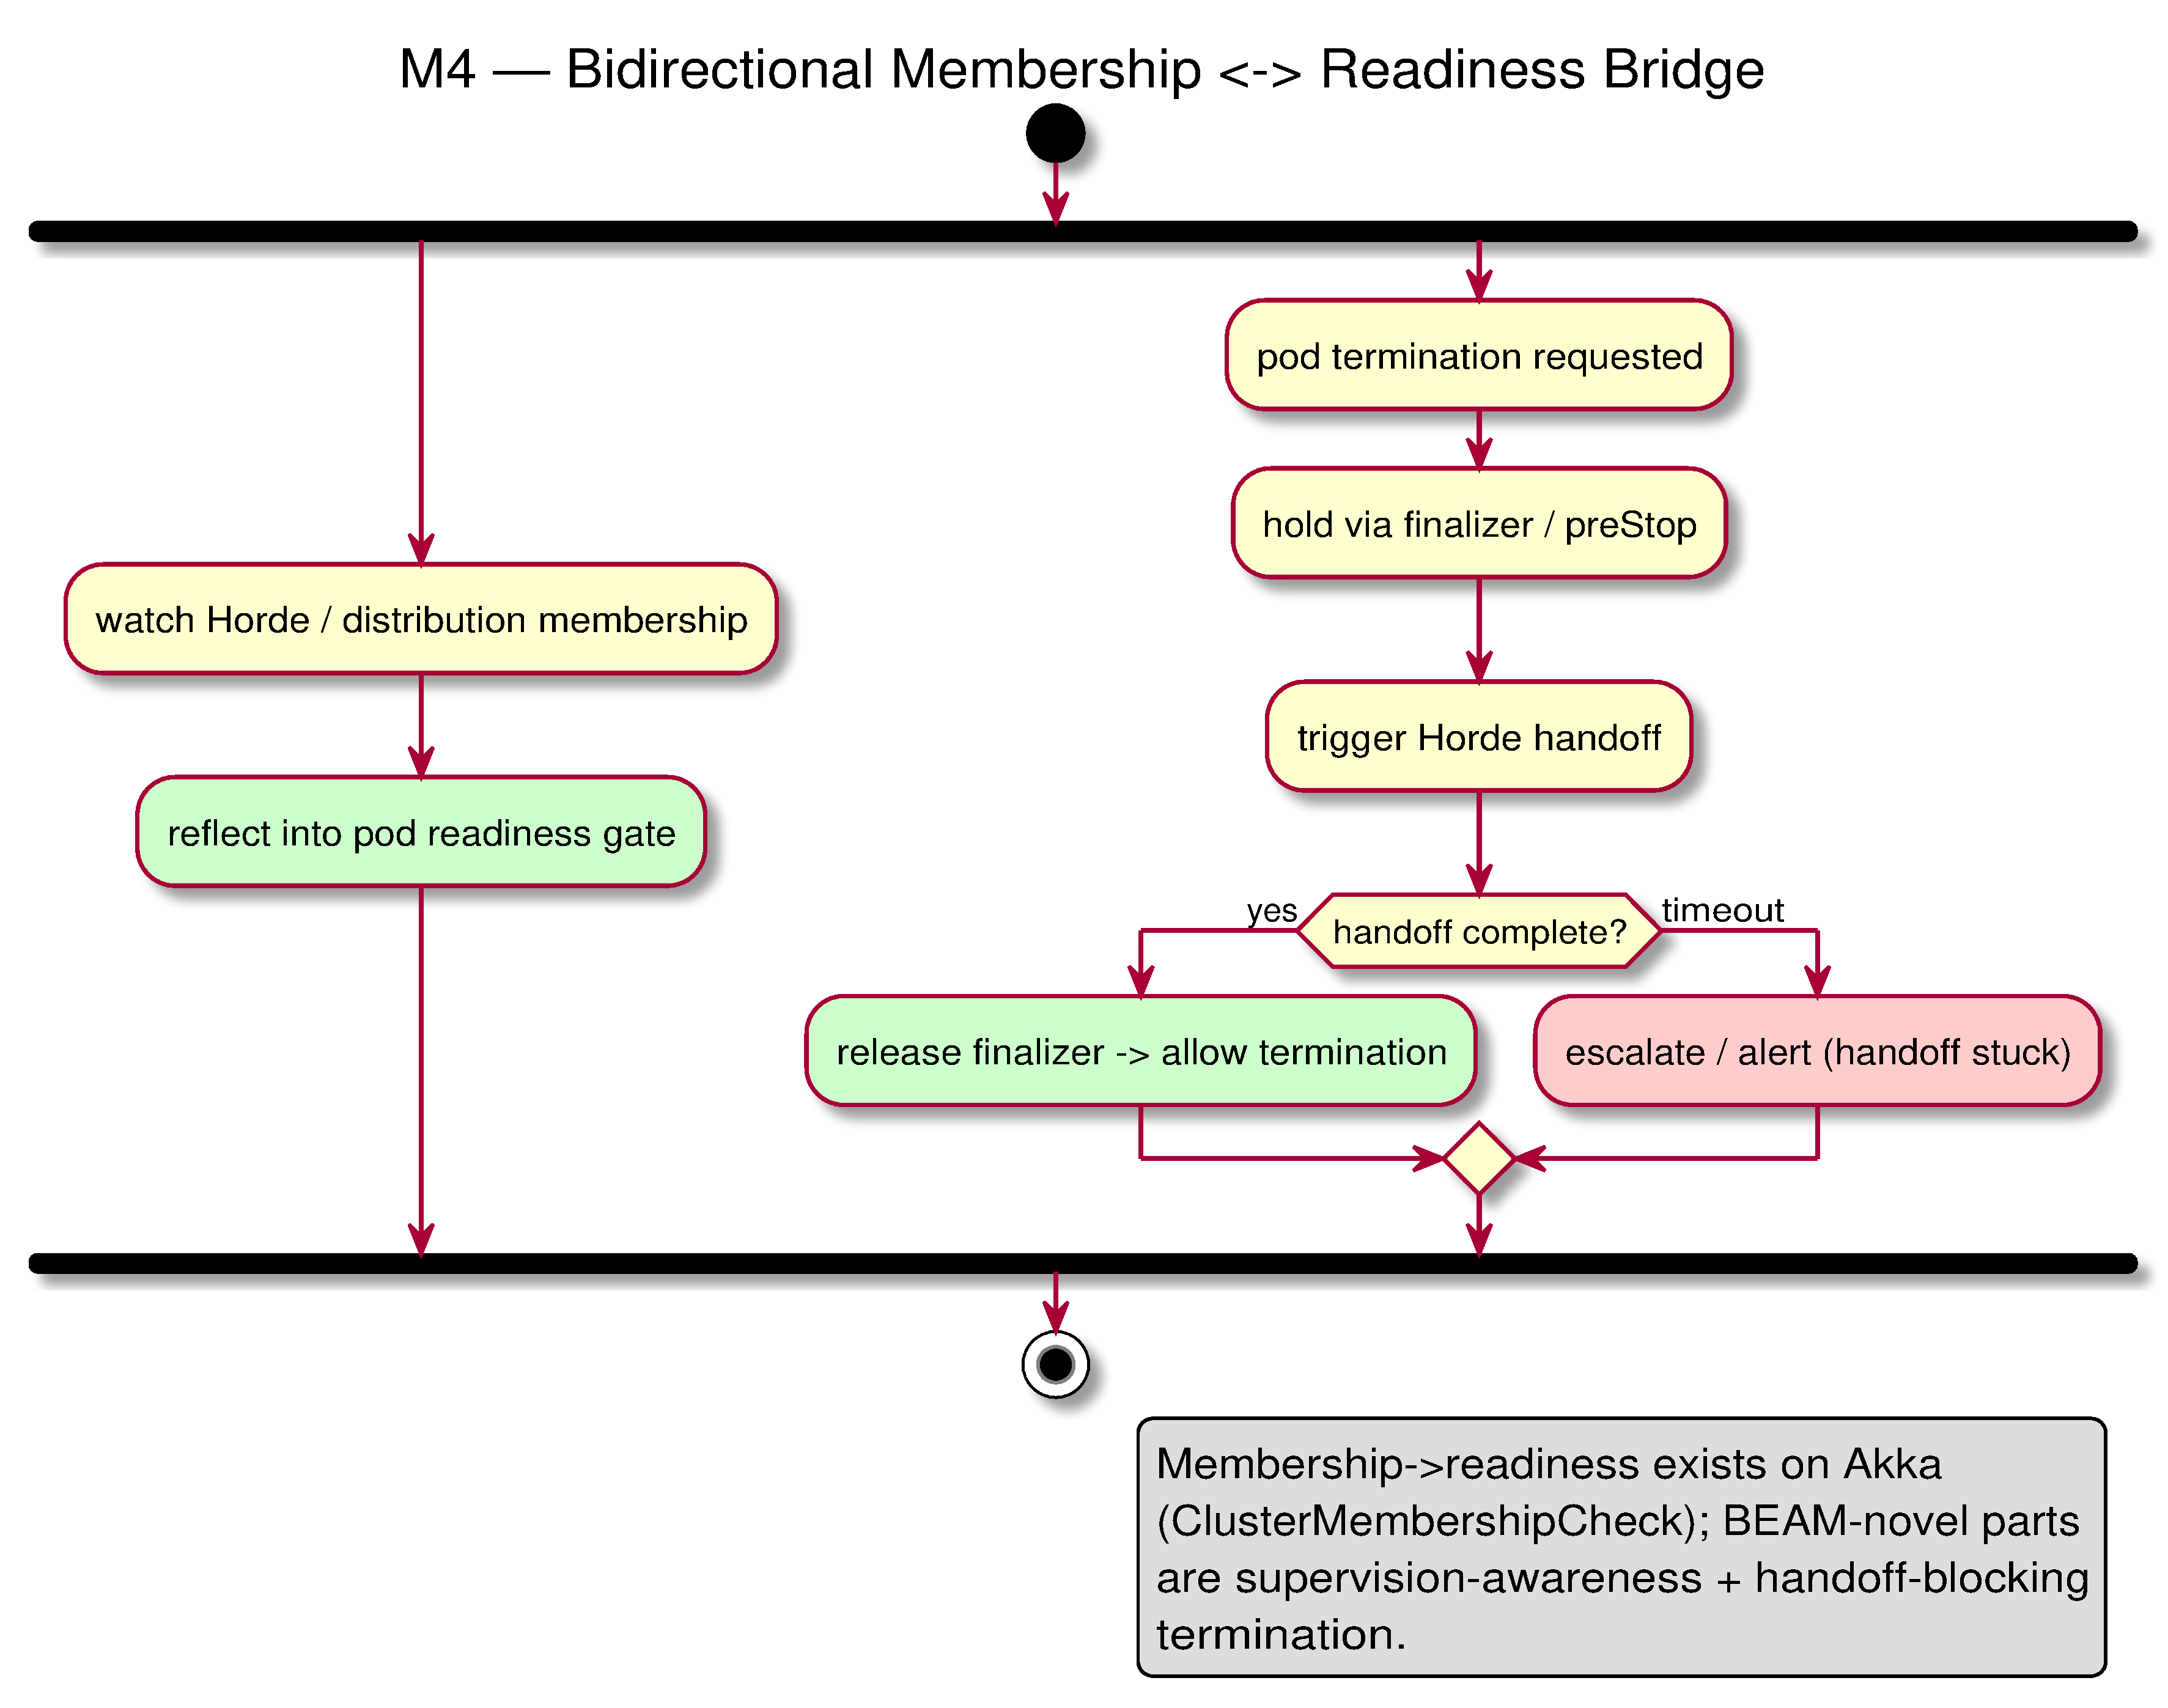
\includegraphics[width=\linewidth,height=0.9\textheight,keepaspectratio]{m4-cluster-aware-operator-activity}
  \caption{M4 (aktivitas): dua jalur paralel---\emph{loop} rekonsiliasi keanggotaan$\rightarrow$\emph{readiness},
  dan penanganan terminasi yang memblokir hingga \emph{handoff} tuntas.}\label{fig:m4-act}\end{figure}
\begin{algorithm}[H]\caption{M4 --- operator + jembatan kesehatan dua arah.}\label{alg:m4}
\begin{algorithmic}[1]
\Loop\ \textsc{Reconcile}
  \State $m \gets$ \Call{WatchMembership}{}; \Call{SetReadinessGate}{$\textit{pod}, m.\textit{up}$}
\EndLoop
\Procedure{OnTerminate}{$\textit{pod}$}
  \State \Call{HoldViaFinalizer}{$\textit{pod}$}; \Call{TriggerHandoff}{}
  \State \textbf{wait until} \Call{HandoffDone}{} \textbf{or} \textit{timeout}
  \State \Call{ReleaseFinalizer}{$\textit{pod}$}
\EndProcedure
\end{algorithmic}\end{algorithm}

\noindent\textbf{Pembahasan.} Diagram sekuens (Gambar~\ref{fig:m4-seq}) menelusuri dua
interaksi: operator membaca keanggotaan Horde lalu menulis \emph{readiness gate} (menutup
Masalah~3), dan saat penghapusan \emph{pod} diminta, ia menahan via \emph{finalizer} sampai
\emph{handoff} selesai (menutup Masalah~4). Diagram aktivitas (Gambar~\ref{fig:m4-act})
memperlihatkan dua jalur paralel tersebut sebagai \emph{fork}. Algoritma~\ref{alg:m4}
memformalkannya: \emph{loop} \textsc{Reconcile} (baris~1--3) terus memantulkan status
\textit{up} ke \emph{readiness gate}; \textsc{OnTerminate} (baris~4--8) menahan via
\emph{finalizer}, memicu \emph{handoff}, menunggu hingga selesai \emph{atau} \emph{timeout},
baru melepas \emph{finalizer}.

\section{M5 --- Arbiter \emph{Split-Brain} via \emph{Lease}/etcd}
\label{sec:m5}
Saat partisi, tiap sisi mencoba mengambil \emph{Kubernetes Lease} (didukung etcd); hanya
pemegang \emph{lease} yang tetap otoritatif, menggantikan \emph{last-writer-wins}
\texttt{:global}. Pola ini sudah ada di Akka sehingga M5 hanya baru sebagai penerapan
khas BEAM.
\begin{figure}[H]\centering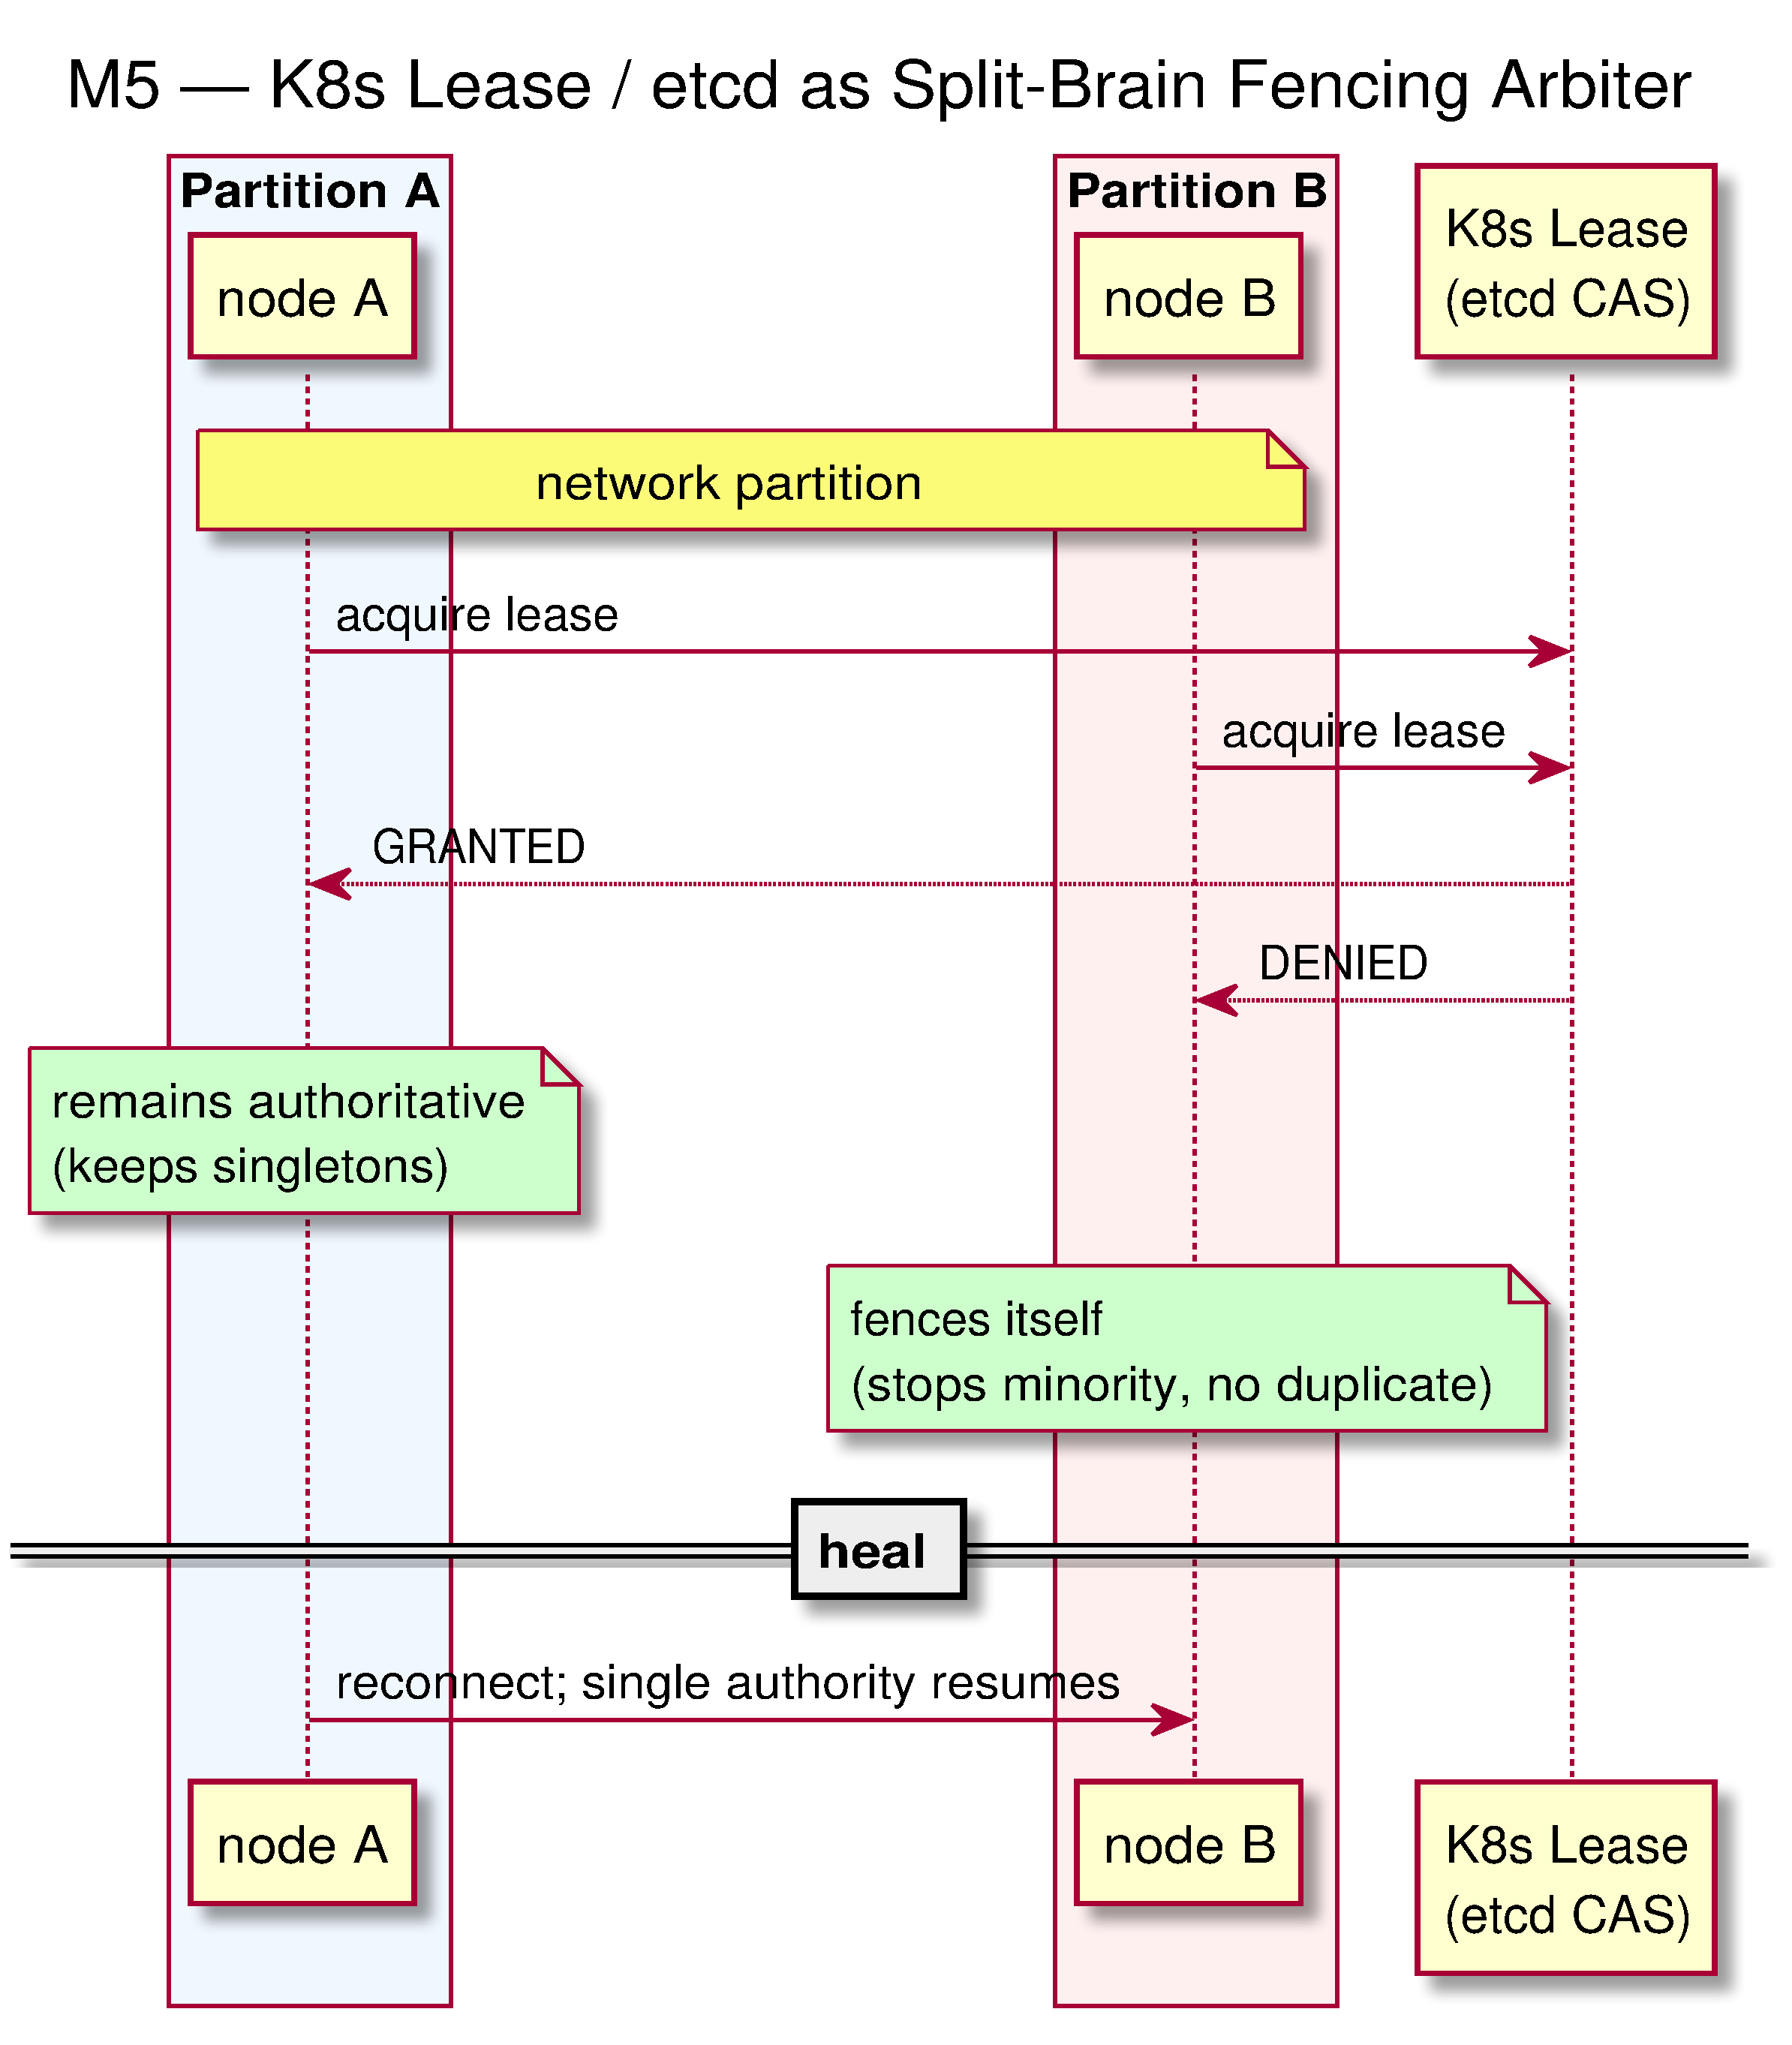
\includegraphics[width=\linewidth,height=0.9\textheight,keepaspectratio]{m5-lease-fencing-arbiter-sequence}
  \caption{M5 (sekuens): kedua sisi partisi memperebutkan \emph{Lease} via etcd CAS; hanya
  pemenang yang \emph{keeps singletons}, sisi minoritas \emph{fences itself}.}\label{fig:m5-seq}\end{figure}
\begin{figure}[H]\centering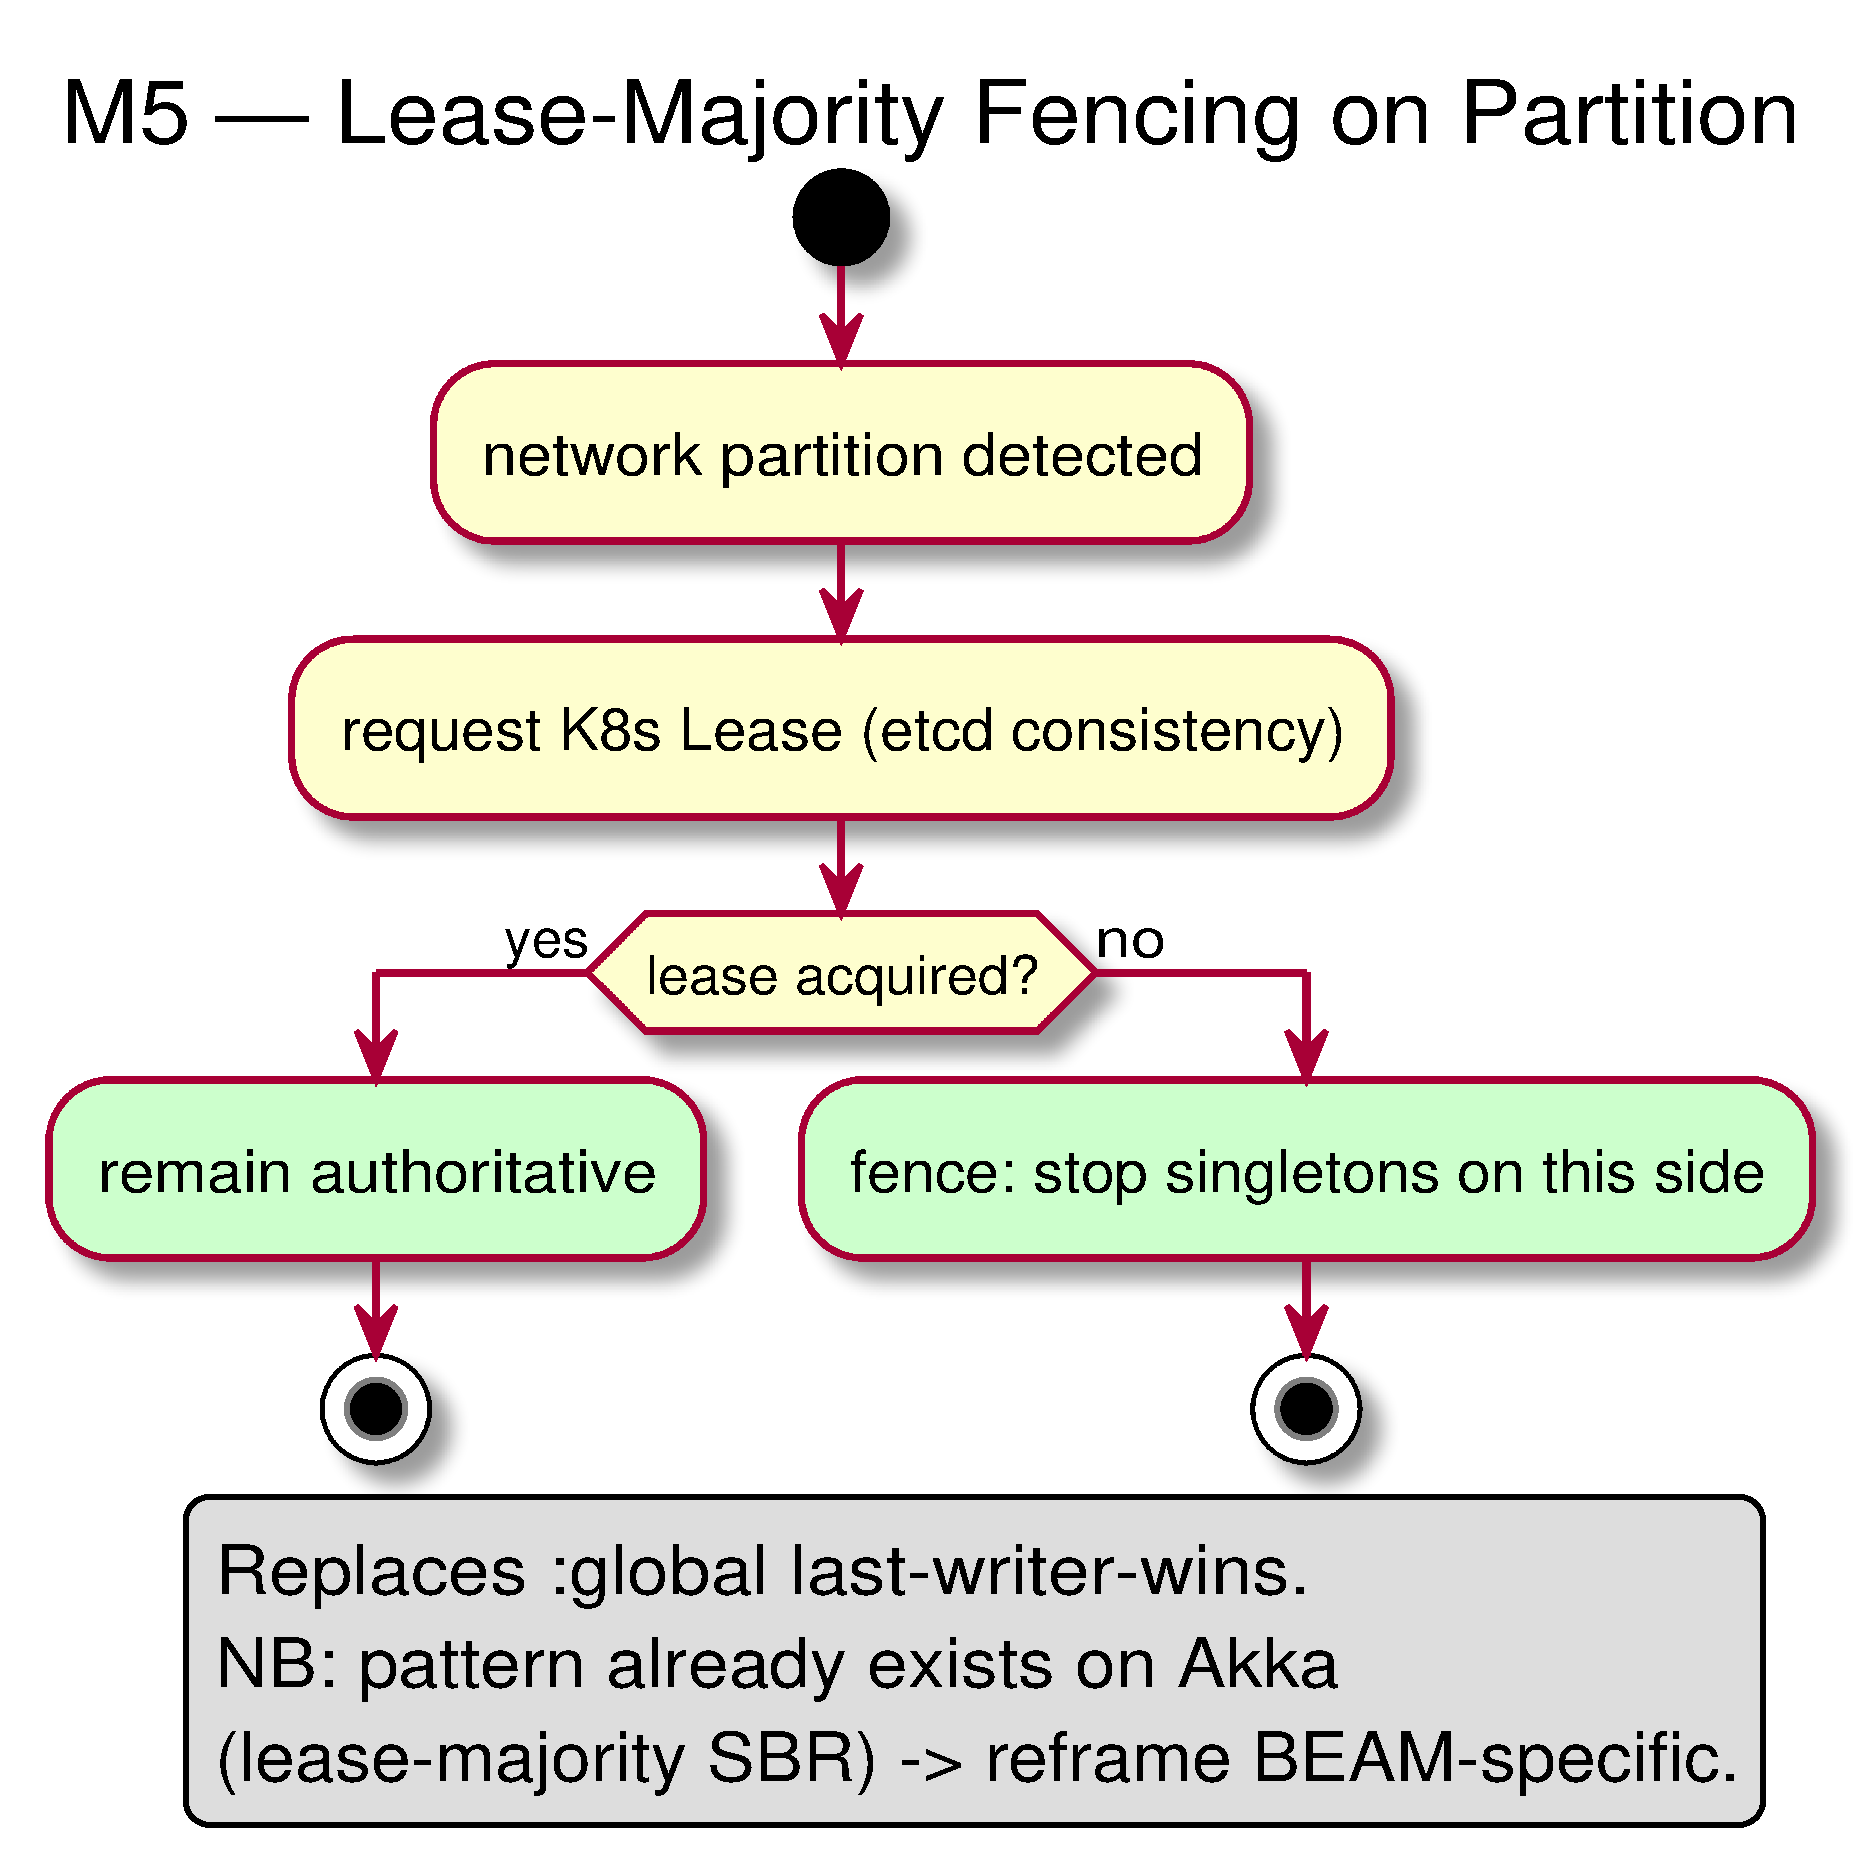
\includegraphics[width=\linewidth,height=0.9\textheight,keepaspectratio]{m5-lease-fencing-arbiter-activity}
  \caption{M5 (aktivitas): keputusan tunggal ``berhasil ambil \emph{lease}?''---ya: tetap
  otoritatif; tidak: \emph{fence}/hentikan \emph{singleton}.}\label{fig:m5-act}\end{figure}
\begin{algorithm}[H]\caption{M5 --- \emph{fencing} \emph{split-brain} via \emph{Lease}.}\label{alg:m5}
\begin{algorithmic}[1]
\Procedure{OnPartition}{}
  \If{\Call{AcquireLease}{\textit{k8sLease}}}
    \State \Call{RemainAuthoritative}{}
  \Else
    \State \Call{StopSingletons}{} \Comment{fence: minoritas mundur}
  \EndIf
\EndProcedure
\end{algorithmic}\end{algorithm}

\noindent\textbf{Pembahasan.} Diagram sekuens (Gambar~\ref{fig:m5-seq}) menggantikan
``kedua sisi mendaftar'' dari Masalah~5 dengan perebutan \emph{Lease}: tiap sisi memanggil
etcd \emph{CAS}, hanya satu yang \texttt{GRANTED} dan menjaga \emph{singleton}-nya,
sementara yang \texttt{DENIED} mem-\emph{fence} diri. Diagram aktivitas
(Gambar~\ref{fig:m5-act}) menyederhanakannya menjadi satu percabangan biner. Algoritma~\ref{alg:m5}
memerincinya: baris~2 mencoba \textsc{AcquireLease}; bila berhasil, baris~3 tetap
otoritatif; selainnya baris~5 menghentikan \emph{singleton} (mundur sebagai minoritas)---
mengganti \emph{last-writer-wins} yang merusak dengan \emph{fencing} terprinsip.

\section{M6 --- Satu Spesifikasi Deklaratif $\rightarrow$ OTP + Manifes K8s}
\label{sec:m6}
Satu spesifikasi toleransi kesalahan dikompilasi menjadi spesifikasi supervisi OTP
\emph{dan} manifes Kubernetes, sebagai sumber kebenaran tunggal yang menghapus \emph{drift}
konfigurasi.
\begin{figure}[H]\centering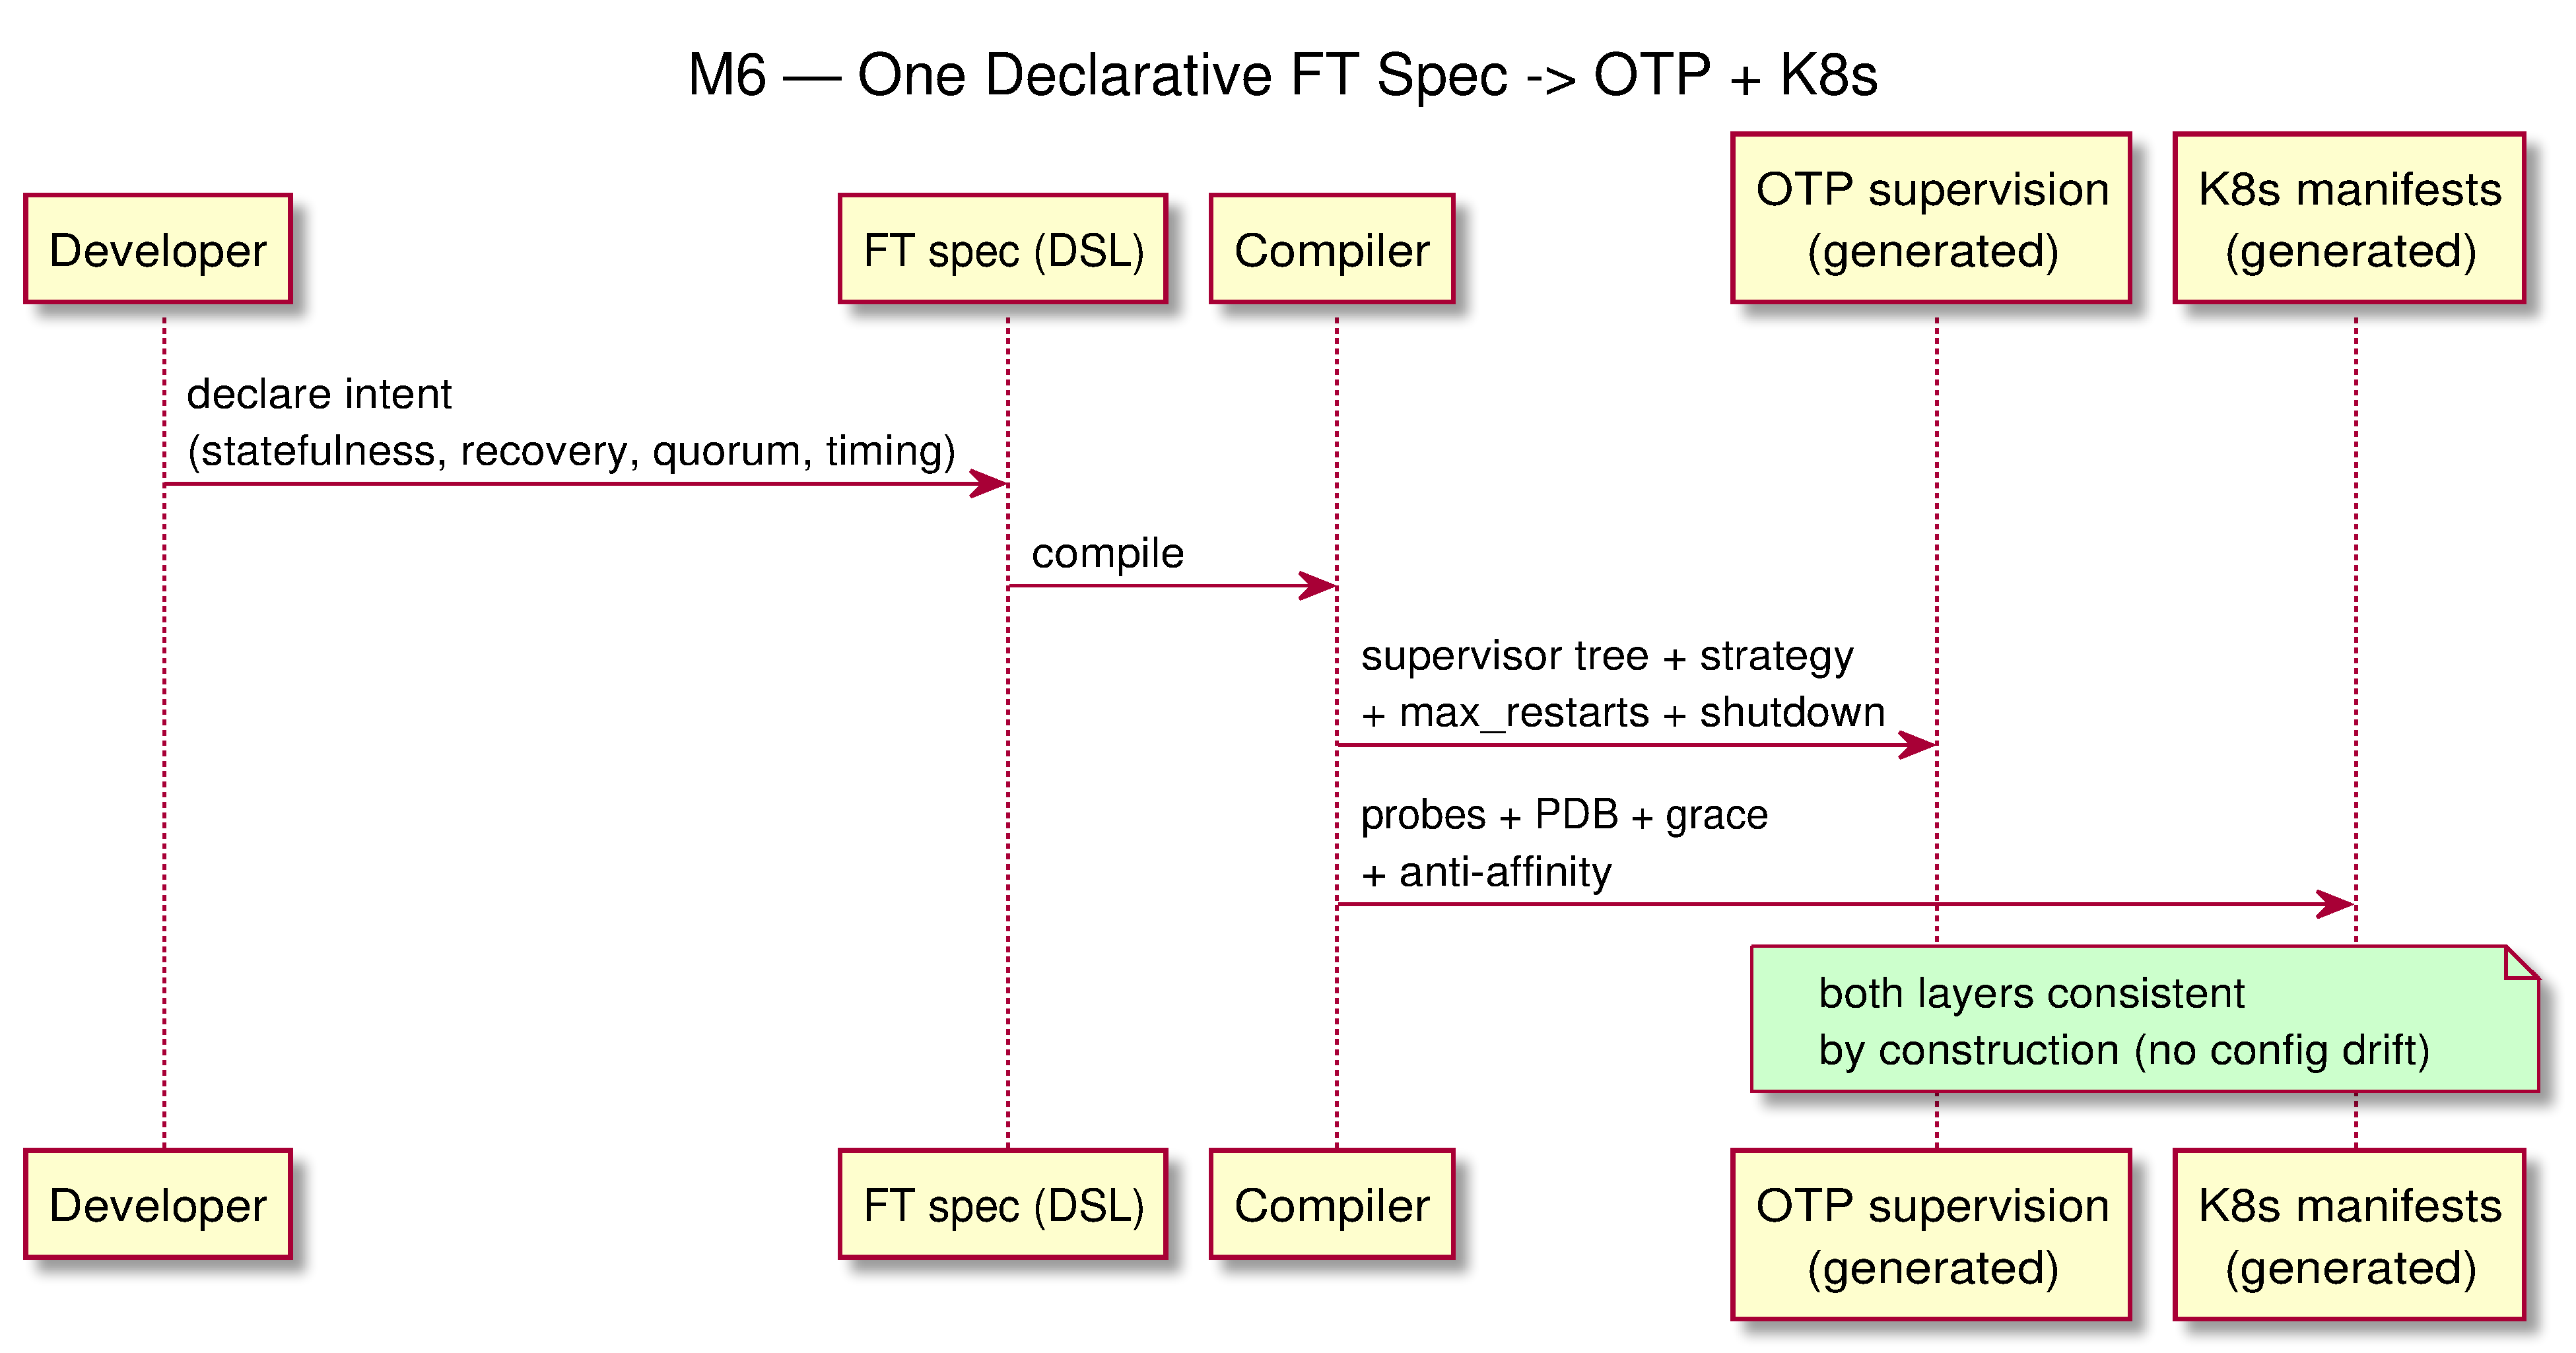
\includegraphics[width=\linewidth,height=0.9\textheight,keepaspectratio]{m6-declarative-spec-compiler-sequence}
  \caption{M6 (sekuens): pengembang menulis satu \emph{FT spec}; \emph{compiler}
  memancarkan spesifikasi supervisi OTP dan manifes Kubernetes yang konsisten.}\label{fig:m6-seq}\end{figure}
\begin{figure}[H]\centering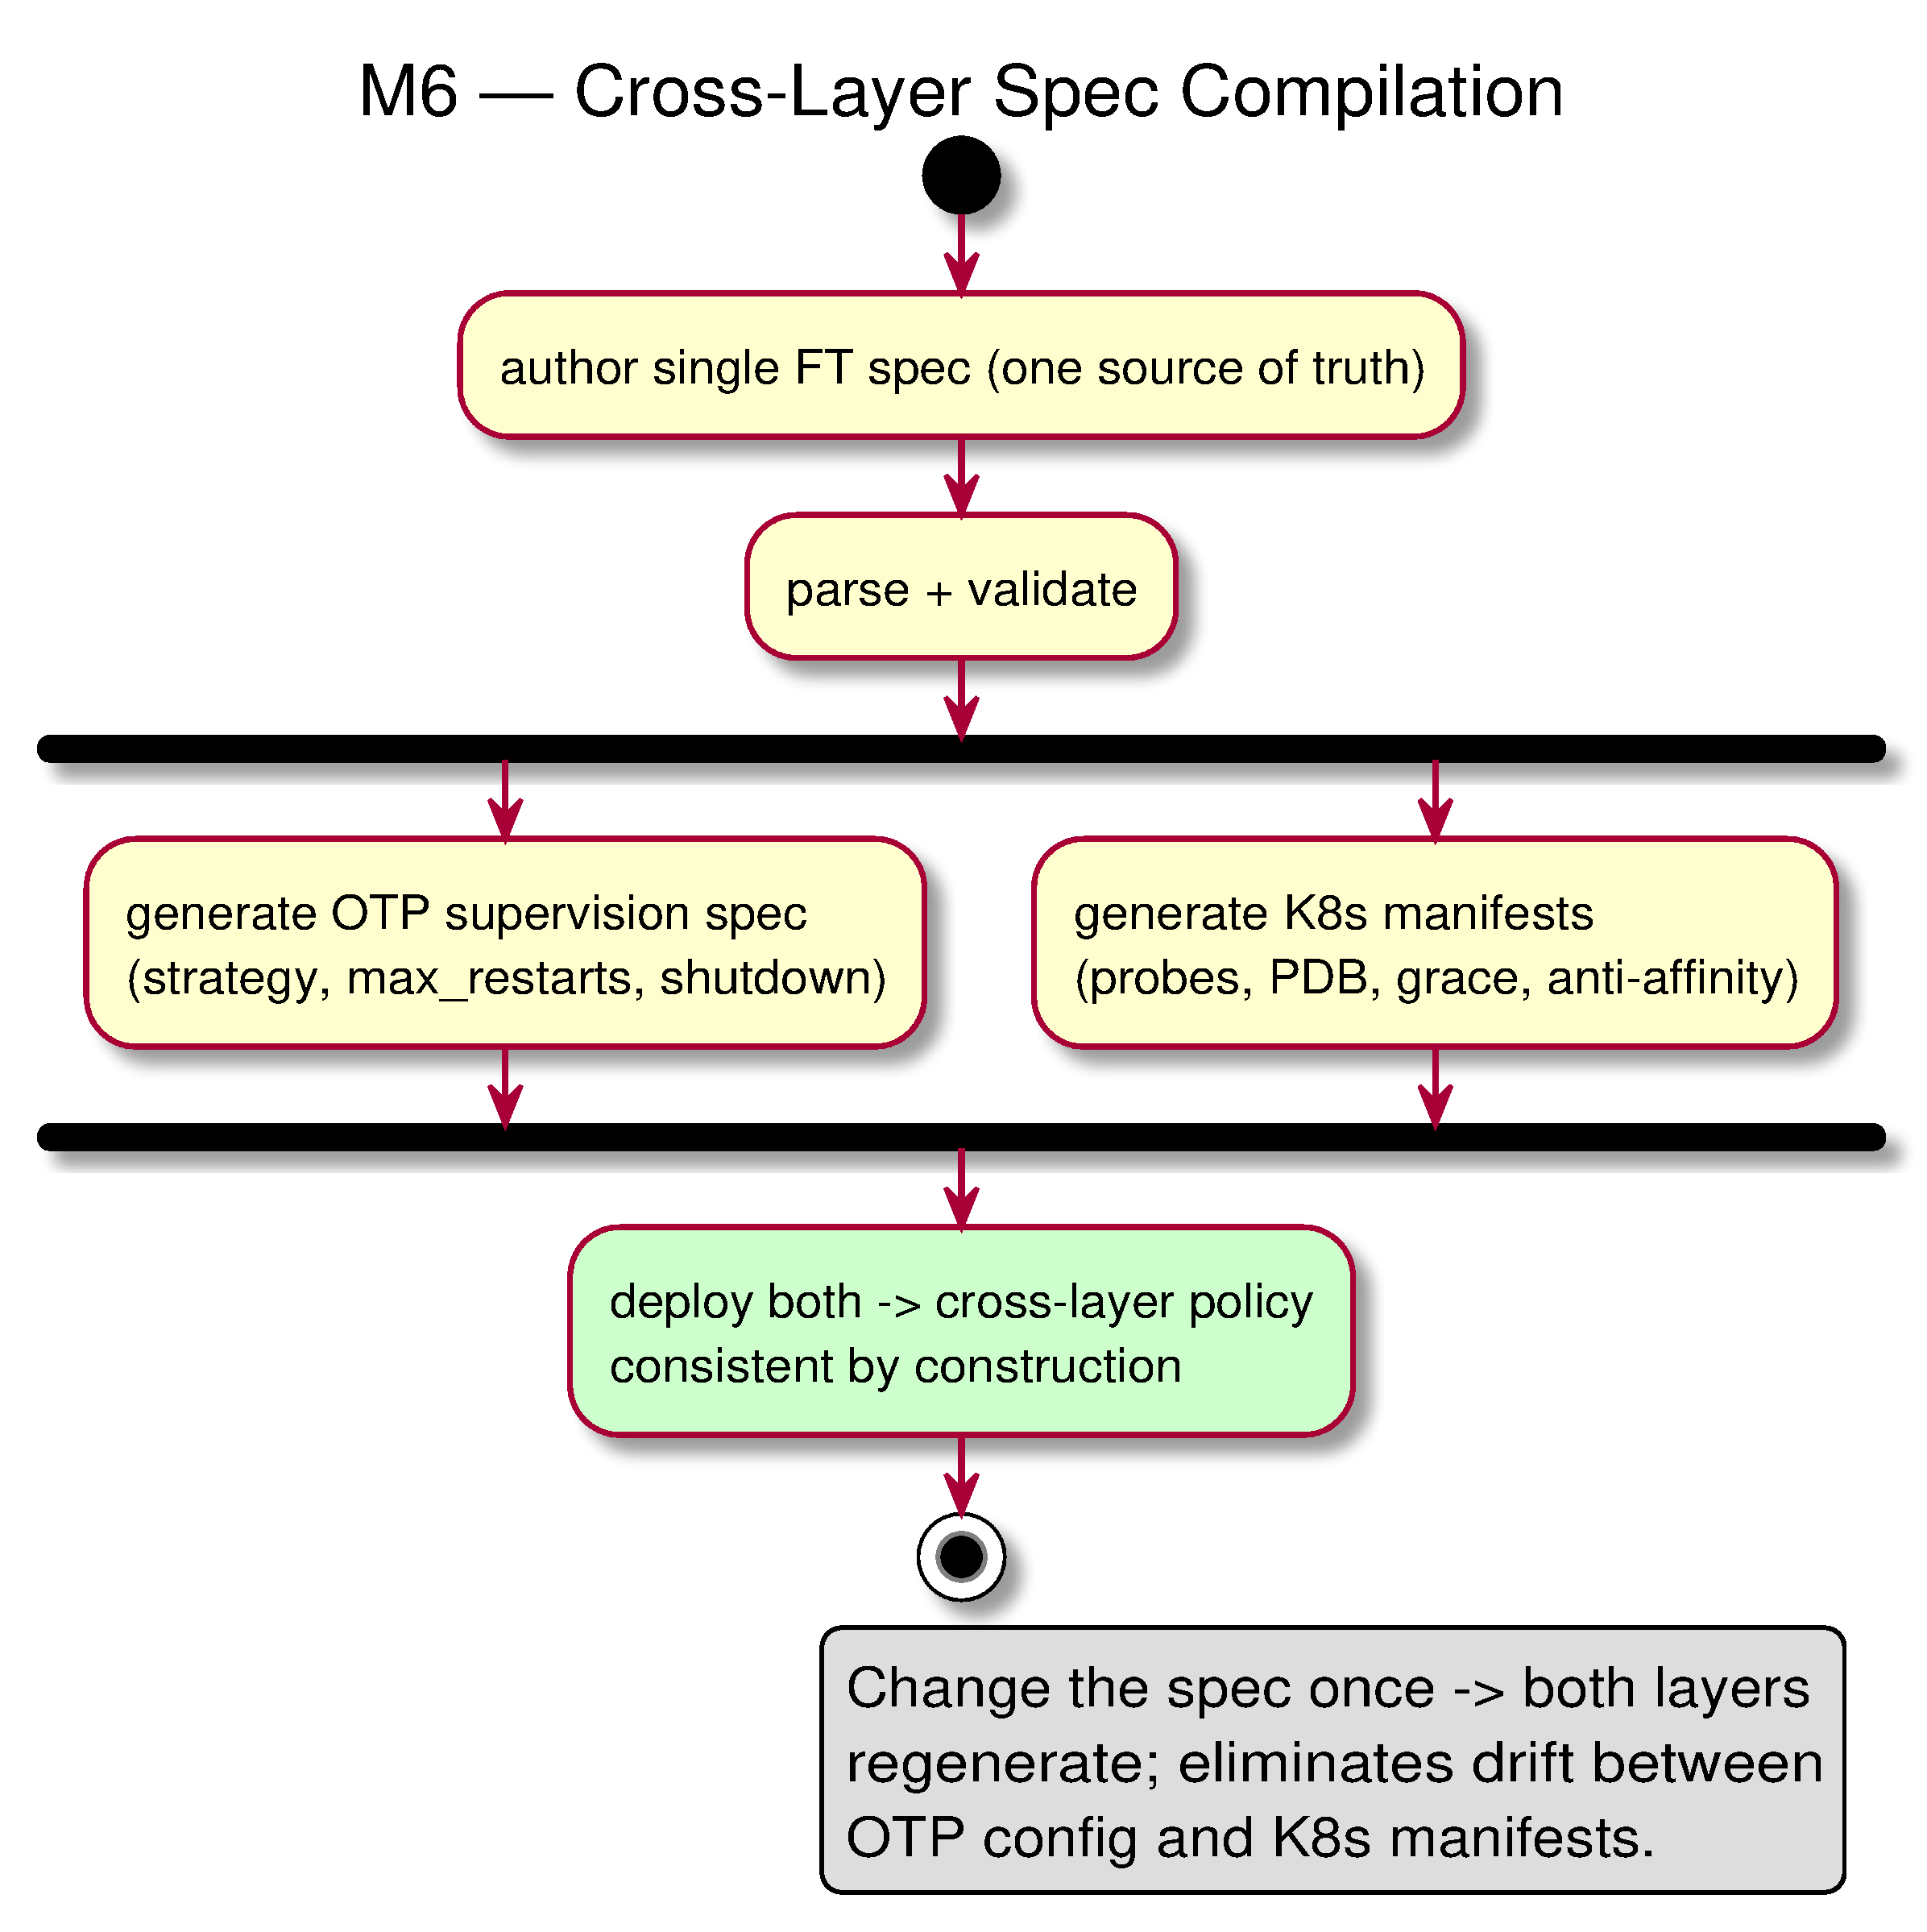
\includegraphics[width=\linewidth,height=0.9\textheight,keepaspectratio]{m6-declarative-spec-compiler-activity}
  \caption{M6 (aktivitas): satu sumber bercabang (\emph{fork}) menjadi dua keluaran lapis,
  sehingga ``ubah spesifikasi sekali'' meregenerasi keduanya.}\label{fig:m6-act}\end{figure}
\begin{algorithm}[H]\caption{M6 --- kompilasi spesifikasi lintas-lapis.}\label{alg:m6}
\begin{algorithmic}[1]
\Function{Compile}{\textit{spec}}
  \State $\textit{otp} \gets$ \Call{GenSupervision}{\textit{spec}} \Comment{strategy, max\_restarts, shutdown}
  \State $\textit{k8s} \gets$ \Call{GenManifests}{\textit{spec}} \Comment{probe, PDB, grace, anti-affinity}
  \State \Return $(\textit{otp}, \textit{k8s})$
\EndFunction
\end{algorithmic}\end{algorithm}

\noindent\textbf{Pembahasan.} Diagram sekuens (Gambar~\ref{fig:m6-seq}) menelusuri alur
penulisan~$\rightarrow$~kompilasi~$\rightarrow$~dua keluaran (OTP dan K8s) dari satu
\emph{spec}. Diagram aktivitas (Gambar~\ref{fig:m6-act}) menampilkannya sebagai
\emph{fork} satu-ke-dua, menegaskan prinsip ``ubah spesifikasi sekali''.
Algoritma~\ref{alg:m6} ringkas namun menyeluruh: baris~2 membangkitkan spesifikasi
supervisi OTP (strategi, \texttt{max\_restarts}, \emph{shutdown}); baris~3 membangkitkan
manifes Kubernetes (\emph{probe}, PDB, \emph{grace}, \emph{anti-affinity}); baris~4
mengembalikan pasangan yang konsisten \emph{by construction}, sehingga \emph{drift}
mustahil terbentuk.

\section{M7 --- PDB/maxUnavailable $\leftrightarrow$ Kuorum BEAM}
\label{sec:m7}
Sebuah pengendali menurunkan \emph{PodDisruptionBudget} (PDB---batas \emph{pod} yang boleh
tak tersedia saat gangguan sukarela)/\texttt{maxUnavailable} dari syarat kuorum dan
kapasitas \emph{handoff} BEAM, sehingga gangguan sukarela tak pernah memutus kuorum.
\begin{figure}[H]\centering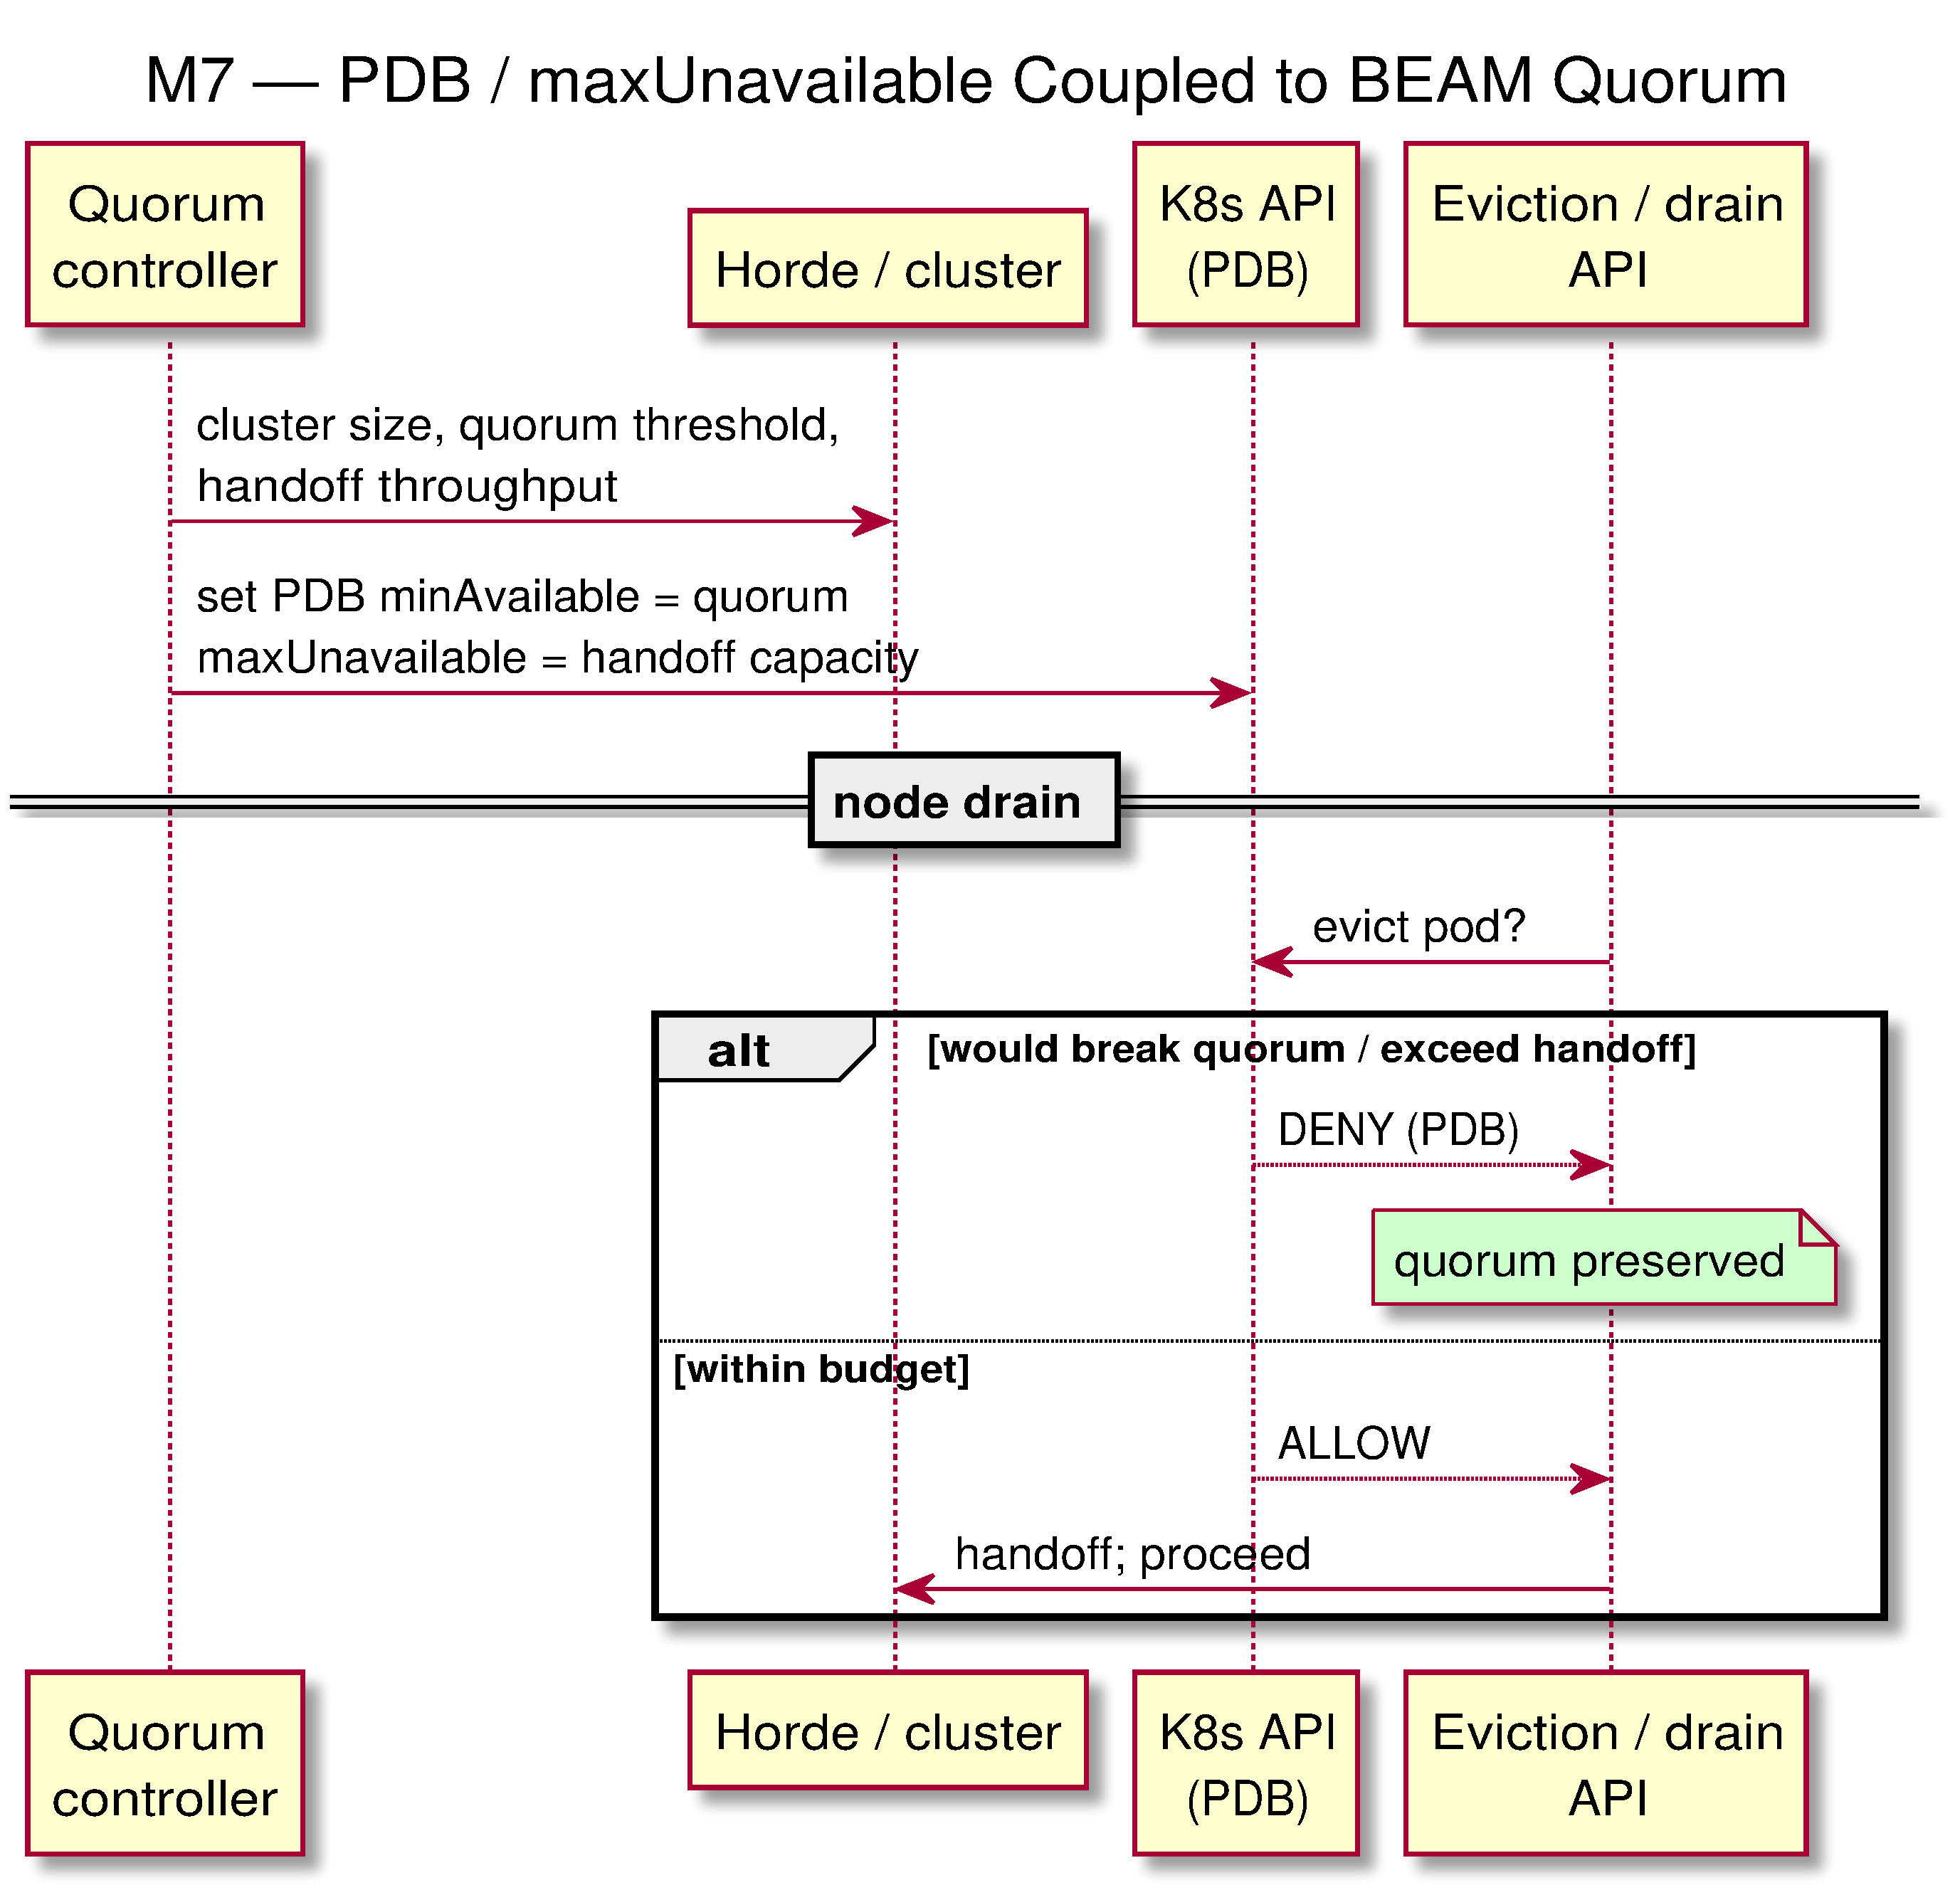
\includegraphics[width=\linewidth,height=0.9\textheight,keepaspectratio]{m7-pdb-quorum-coupling-sequence}
  \caption{M7 (sekuens): \emph{quorum controller} menetapkan PDB dari kuorum/kapasitas
  \emph{handoff}; saat \emph{eviction}, API menolak bila kuorum akan pecah.}\label{fig:m7-seq}\end{figure}
\begin{figure}[H]\centering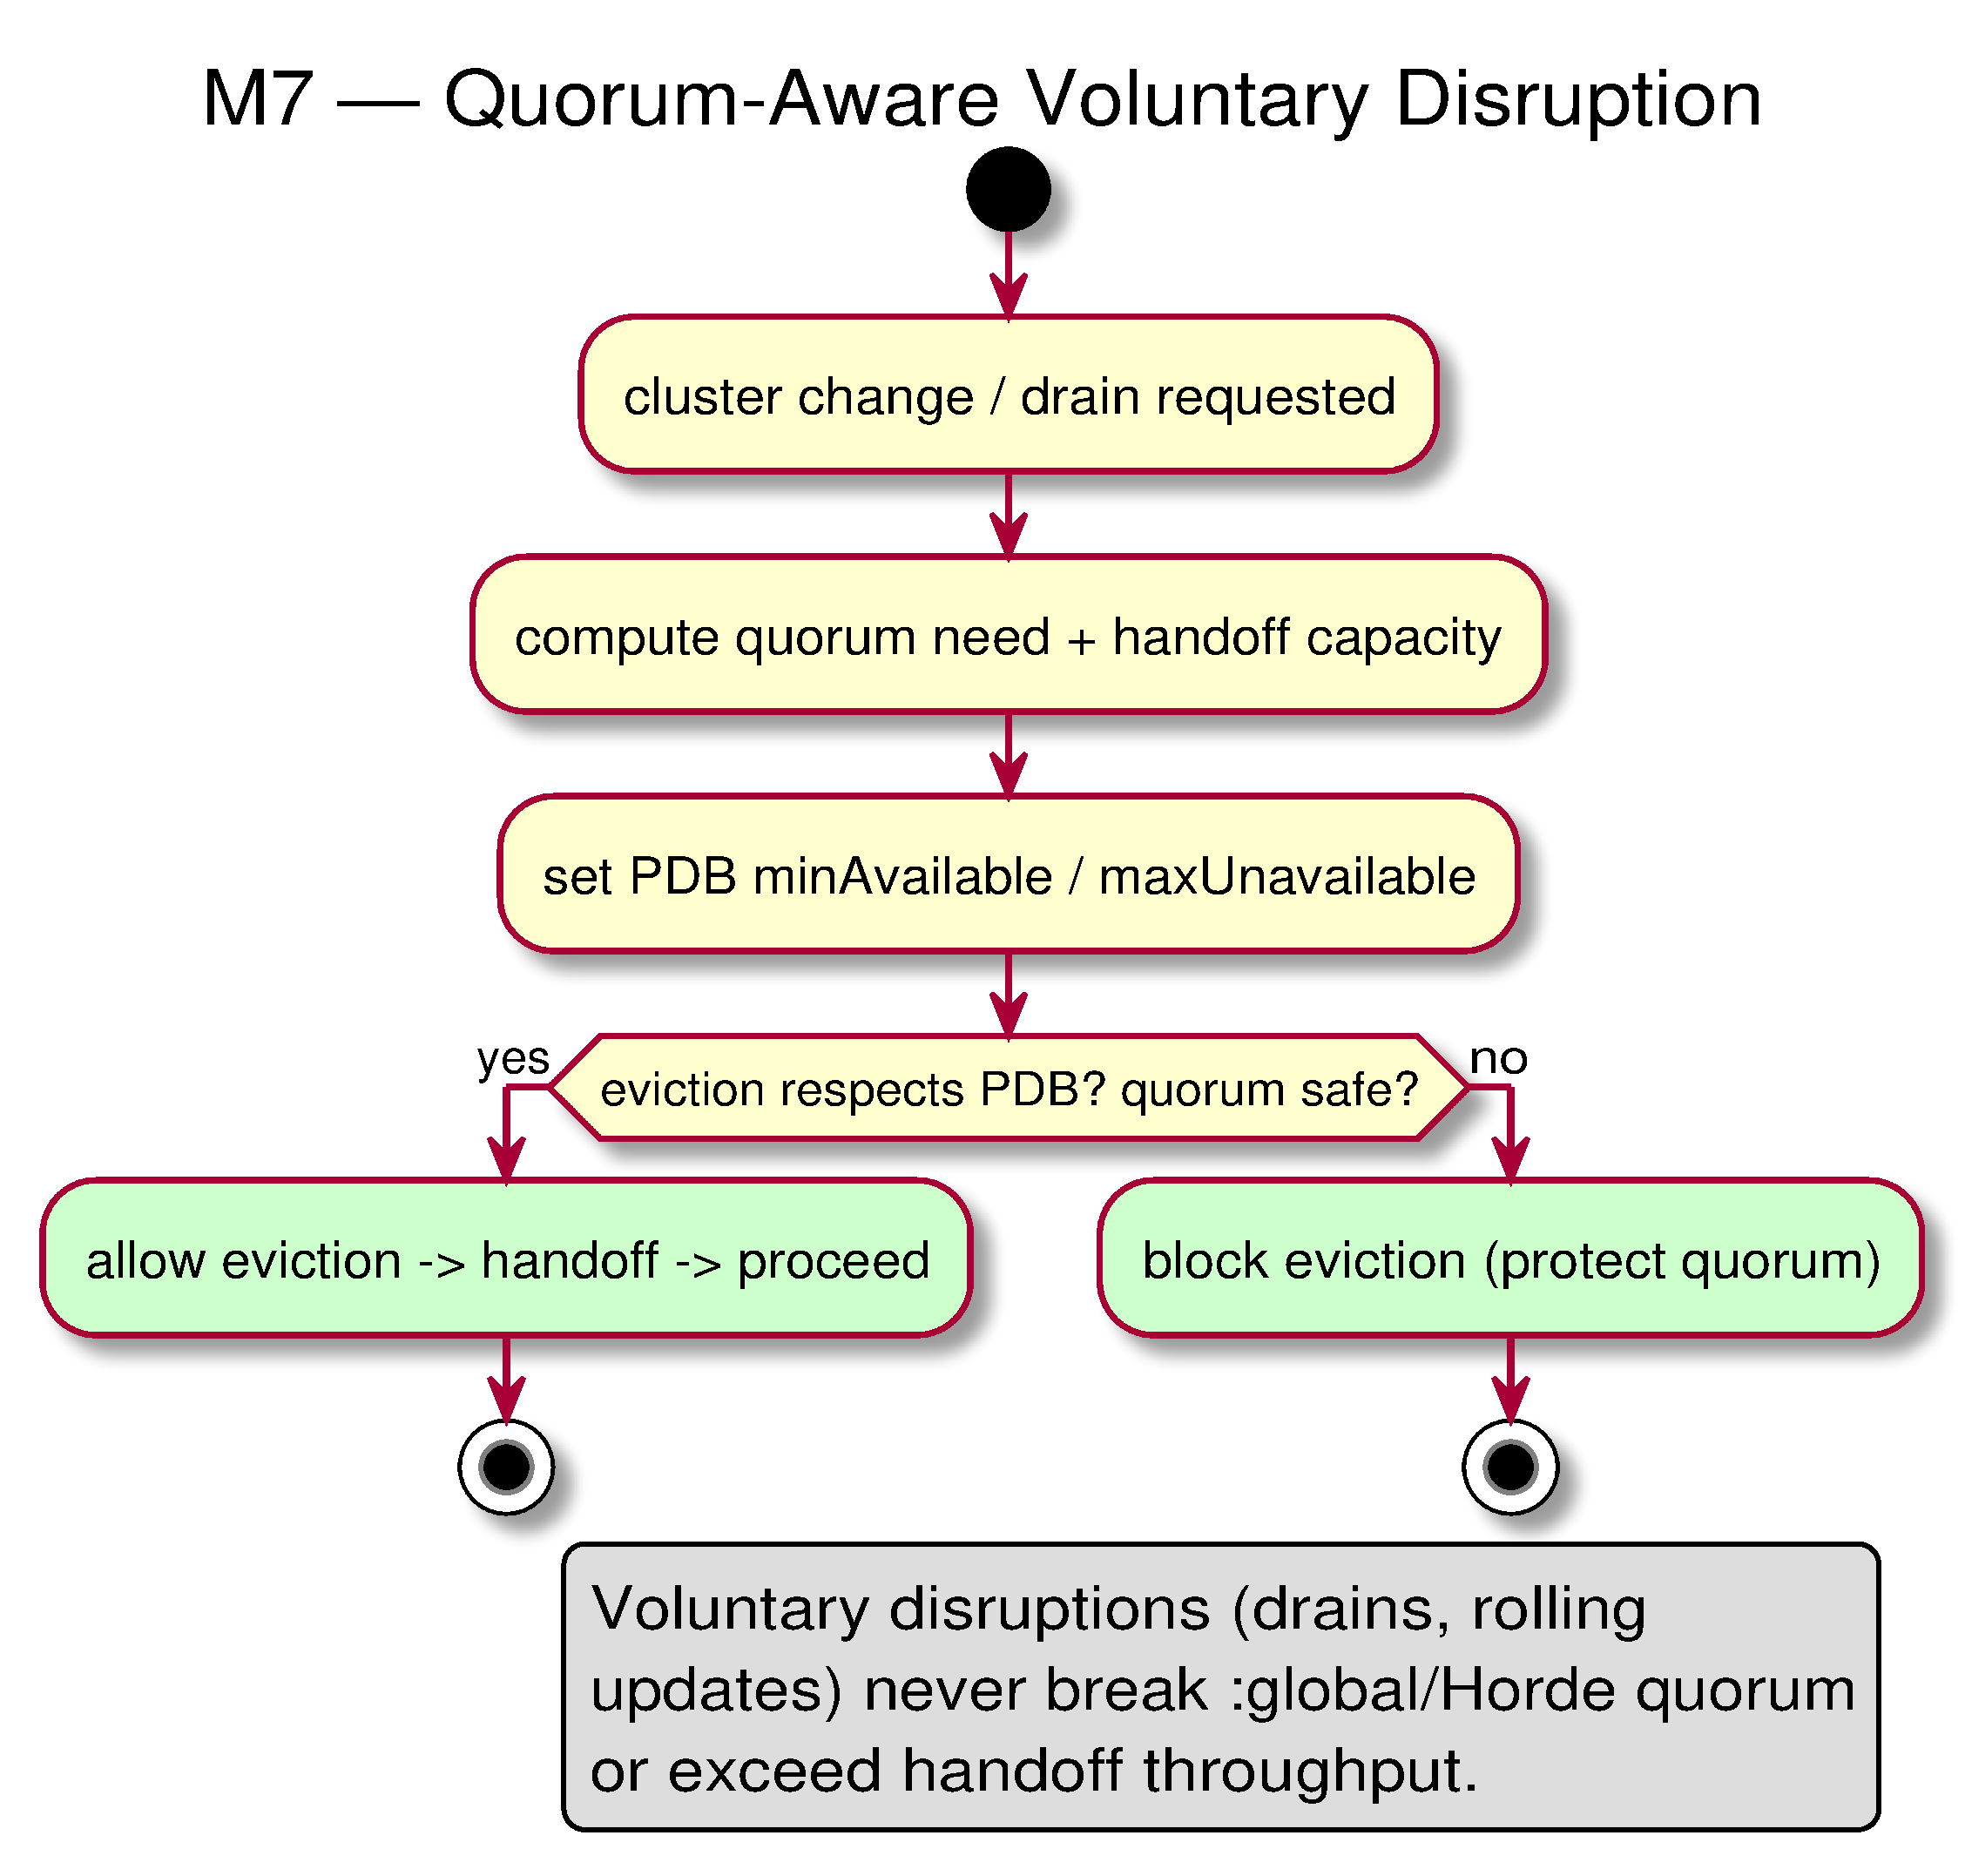
\includegraphics[width=\linewidth,height=0.9\textheight,keepaspectratio]{m7-pdb-quorum-coupling-activity}
  \caption{M7 (aktivitas): gangguan sukarela diizinkan hanya bila tetap menghormati kuorum;
  selainnya \emph{eviction} diblokir.}\label{fig:m7-act}\end{figure}
\begin{algorithm}[H]\caption{M7 --- kopling PDB ke kuorum BEAM.}\label{alg:m7}
\begin{algorithmic}[1]
\Procedure{OnClusterChange}{}
  \State \Call{SetPDB}{\textit{minAvailable}{=}\textsc{Quorum}(),\ \textit{maxUnavailable}{=}\textsc{HandoffCap}()}
\EndProcedure
\Procedure{OnEviction}{\textit{pod}}
  \If{\Call{ViolatesQuorum}{\textit{pod}}} \State \Call{Deny}{} \Else\ \State \Call{Allow}{}; \Call{Handoff}{} \EndIf
\EndProcedure
\end{algorithmic}\end{algorithm}

\noindent\textbf{Pembahasan.} Diagram sekuens (Gambar~\ref{fig:m7-seq}) menelusuri
\emph{quorum controller} yang membaca ukuran \emph{cluster}, ambang kuorum, dan kapasitas
\emph{handoff}, lalu menulis PDB; ketika \emph{eviction/drain API} meminta pengusiran,
keputusan \emph{allow}/\emph{block} mengalir balik. Diagram aktivitas
(Gambar~\ref{fig:m7-act}) menempatkan keputusan pada ``\emph{eviction} menghormati PDB
(kuorum aman)?''. Algoritma~\ref{alg:m7} memformalkannya dalam dua prosedur:
\textsc{OnClusterChange} (baris~2) menyetel \texttt{minAvailable} ke kuorum dan
\texttt{maxUnavailable} ke kapasitas \emph{handoff}; \textsc{OnEviction} (baris~4--6)
menolak bila melanggar kuorum, selainnya mengizinkan lalu mela\-kukan \emph{handoff}.

\section{M8 --- Eskalasi \emph{Restart-Budget} Adaptif $\leftrightarrow$ \emph{Backoff} K8s}
\label{sec:m8}
Sebuah pengendali menyetel \texttt{max\_restarts}/\texttt{max\_seconds} OTP menurut laju
kegagalan teramati dan memetakan batas eskalasi ke \emph{restart}/\emph{backoff} Kubernetes.
\begin{figure}[H]\centering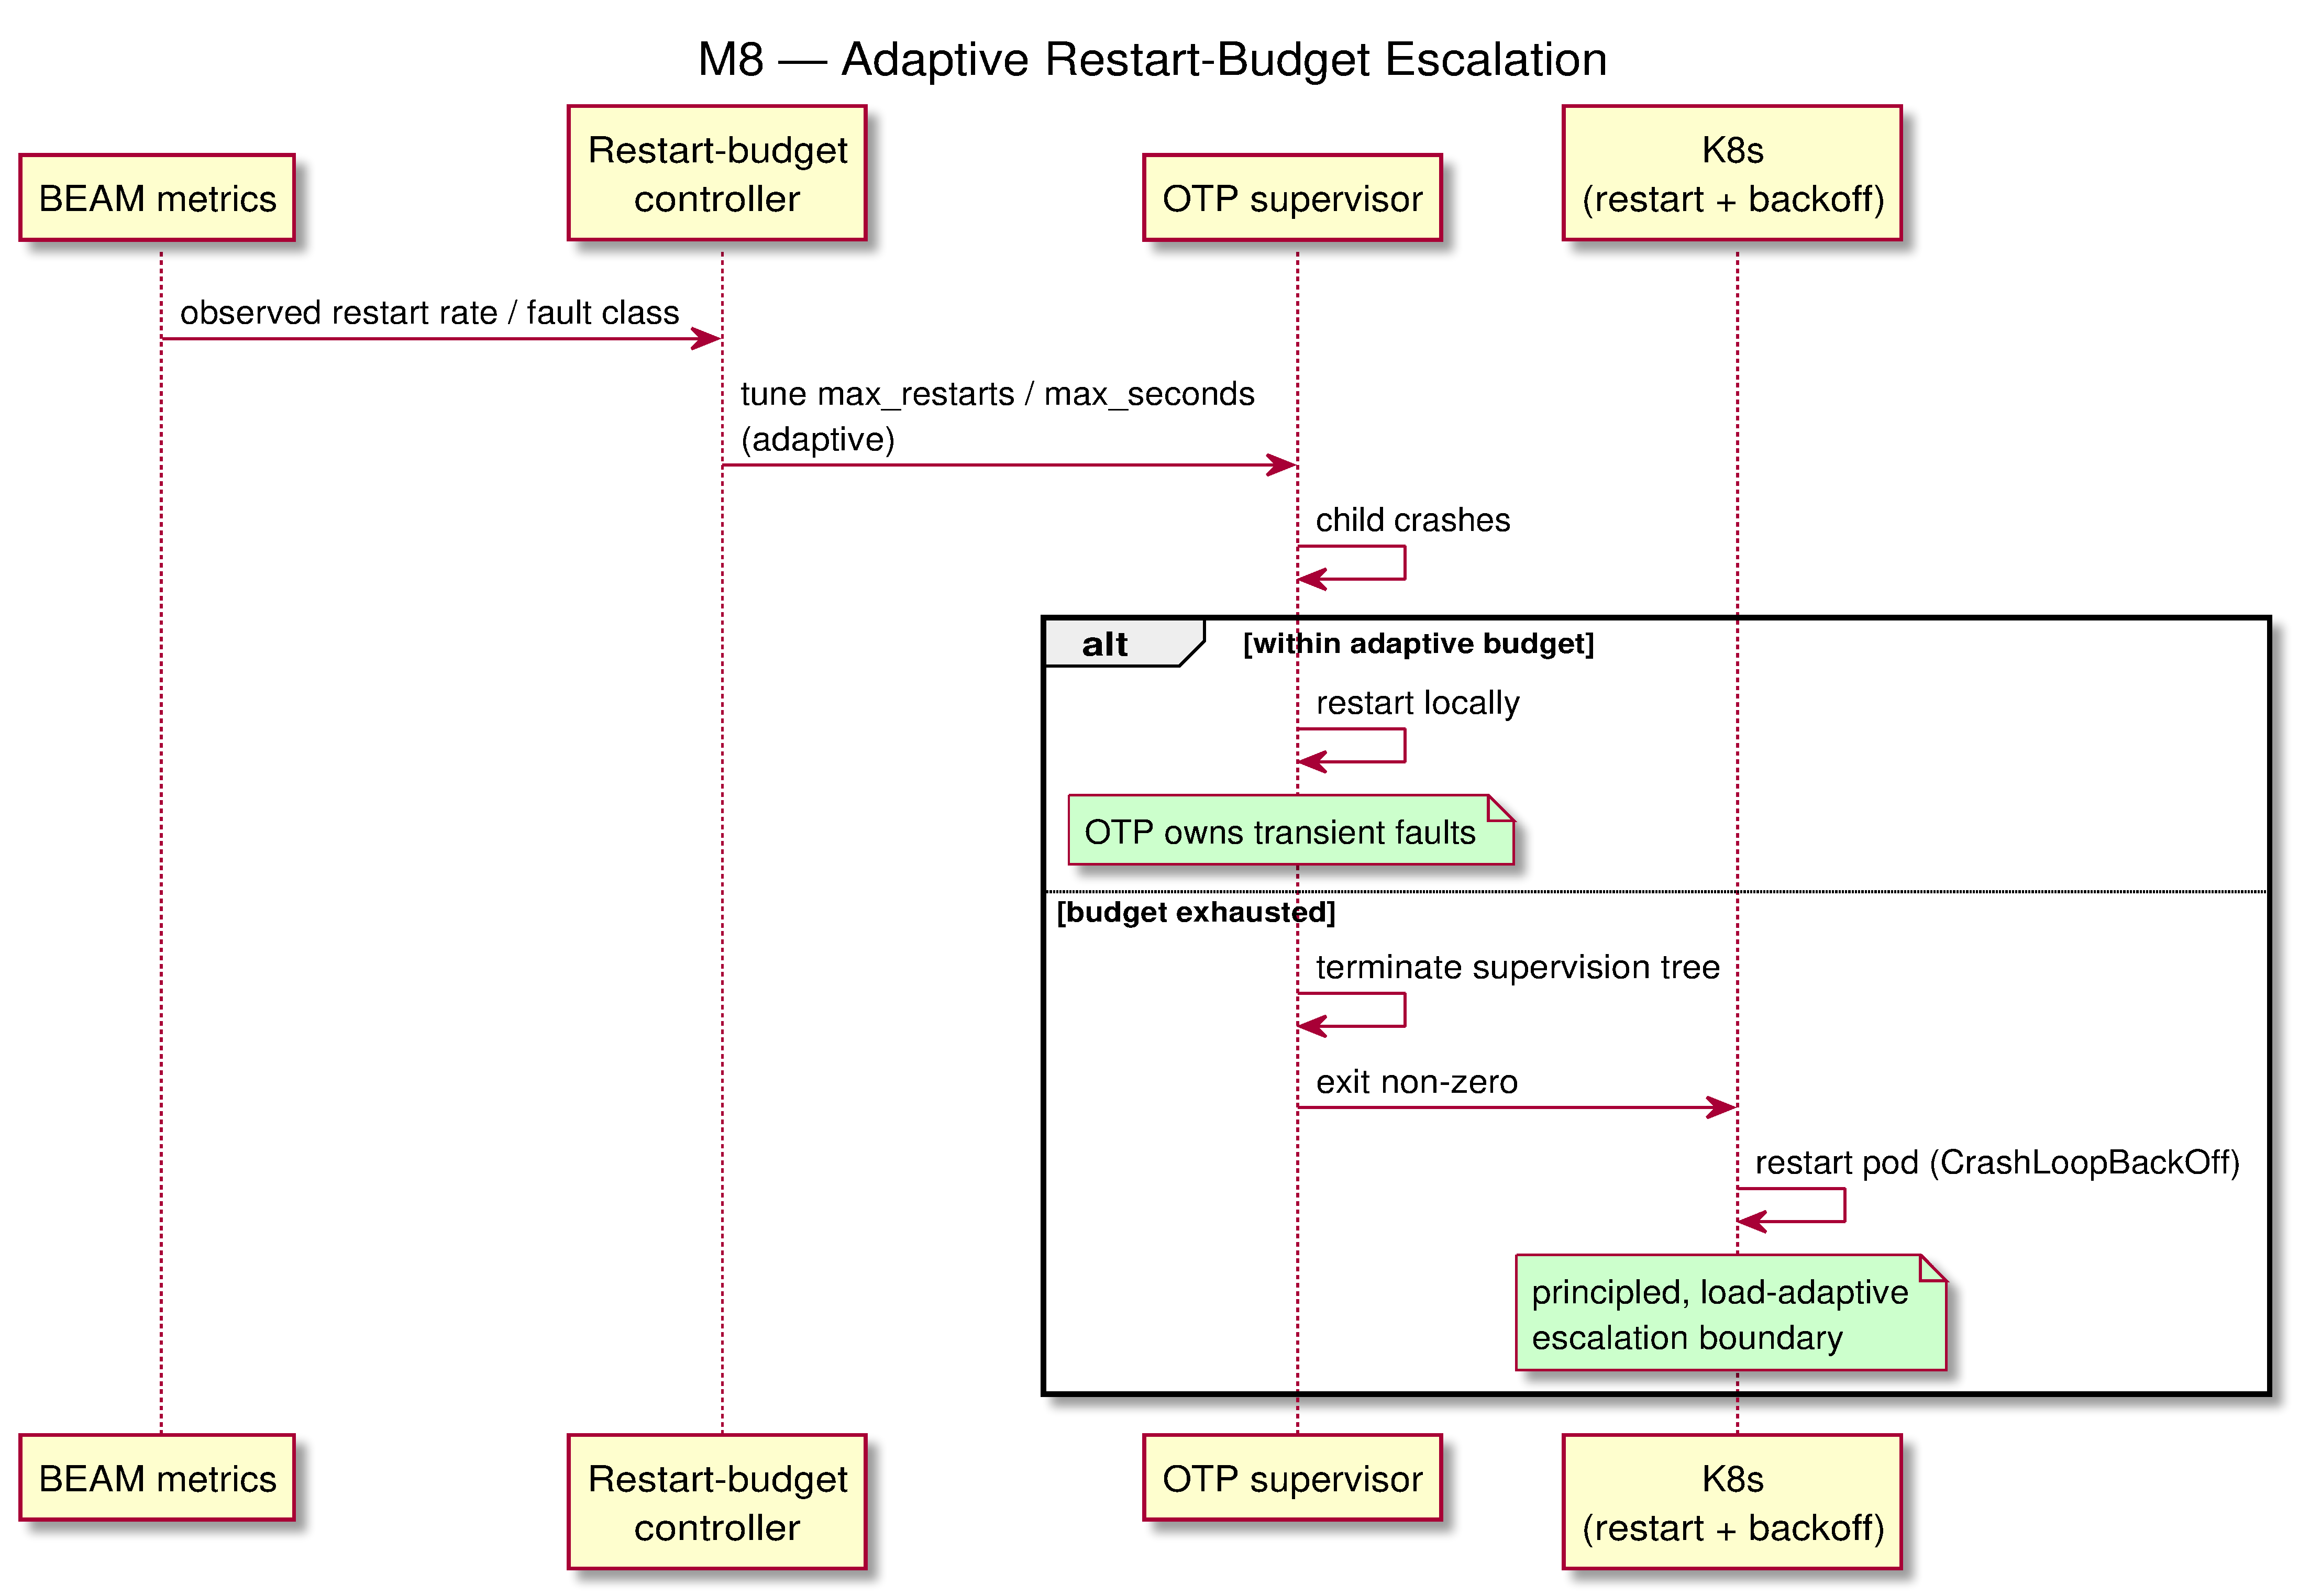
\includegraphics[width=\linewidth,height=0.9\textheight,keepaspectratio]{m8-adaptive-restart-budget-sequence}
  \caption{M8 (sekuens): pengendali menyesuaikan jatah \emph{restart} dari \emph{fault rate};
  saat jatah habis, VM keluar non-nol dan Kubernetes me-\emph{restart} dengan \emph{backoff}.}\label{fig:m8-seq}\end{figure}
\begin{figure}[H]\centering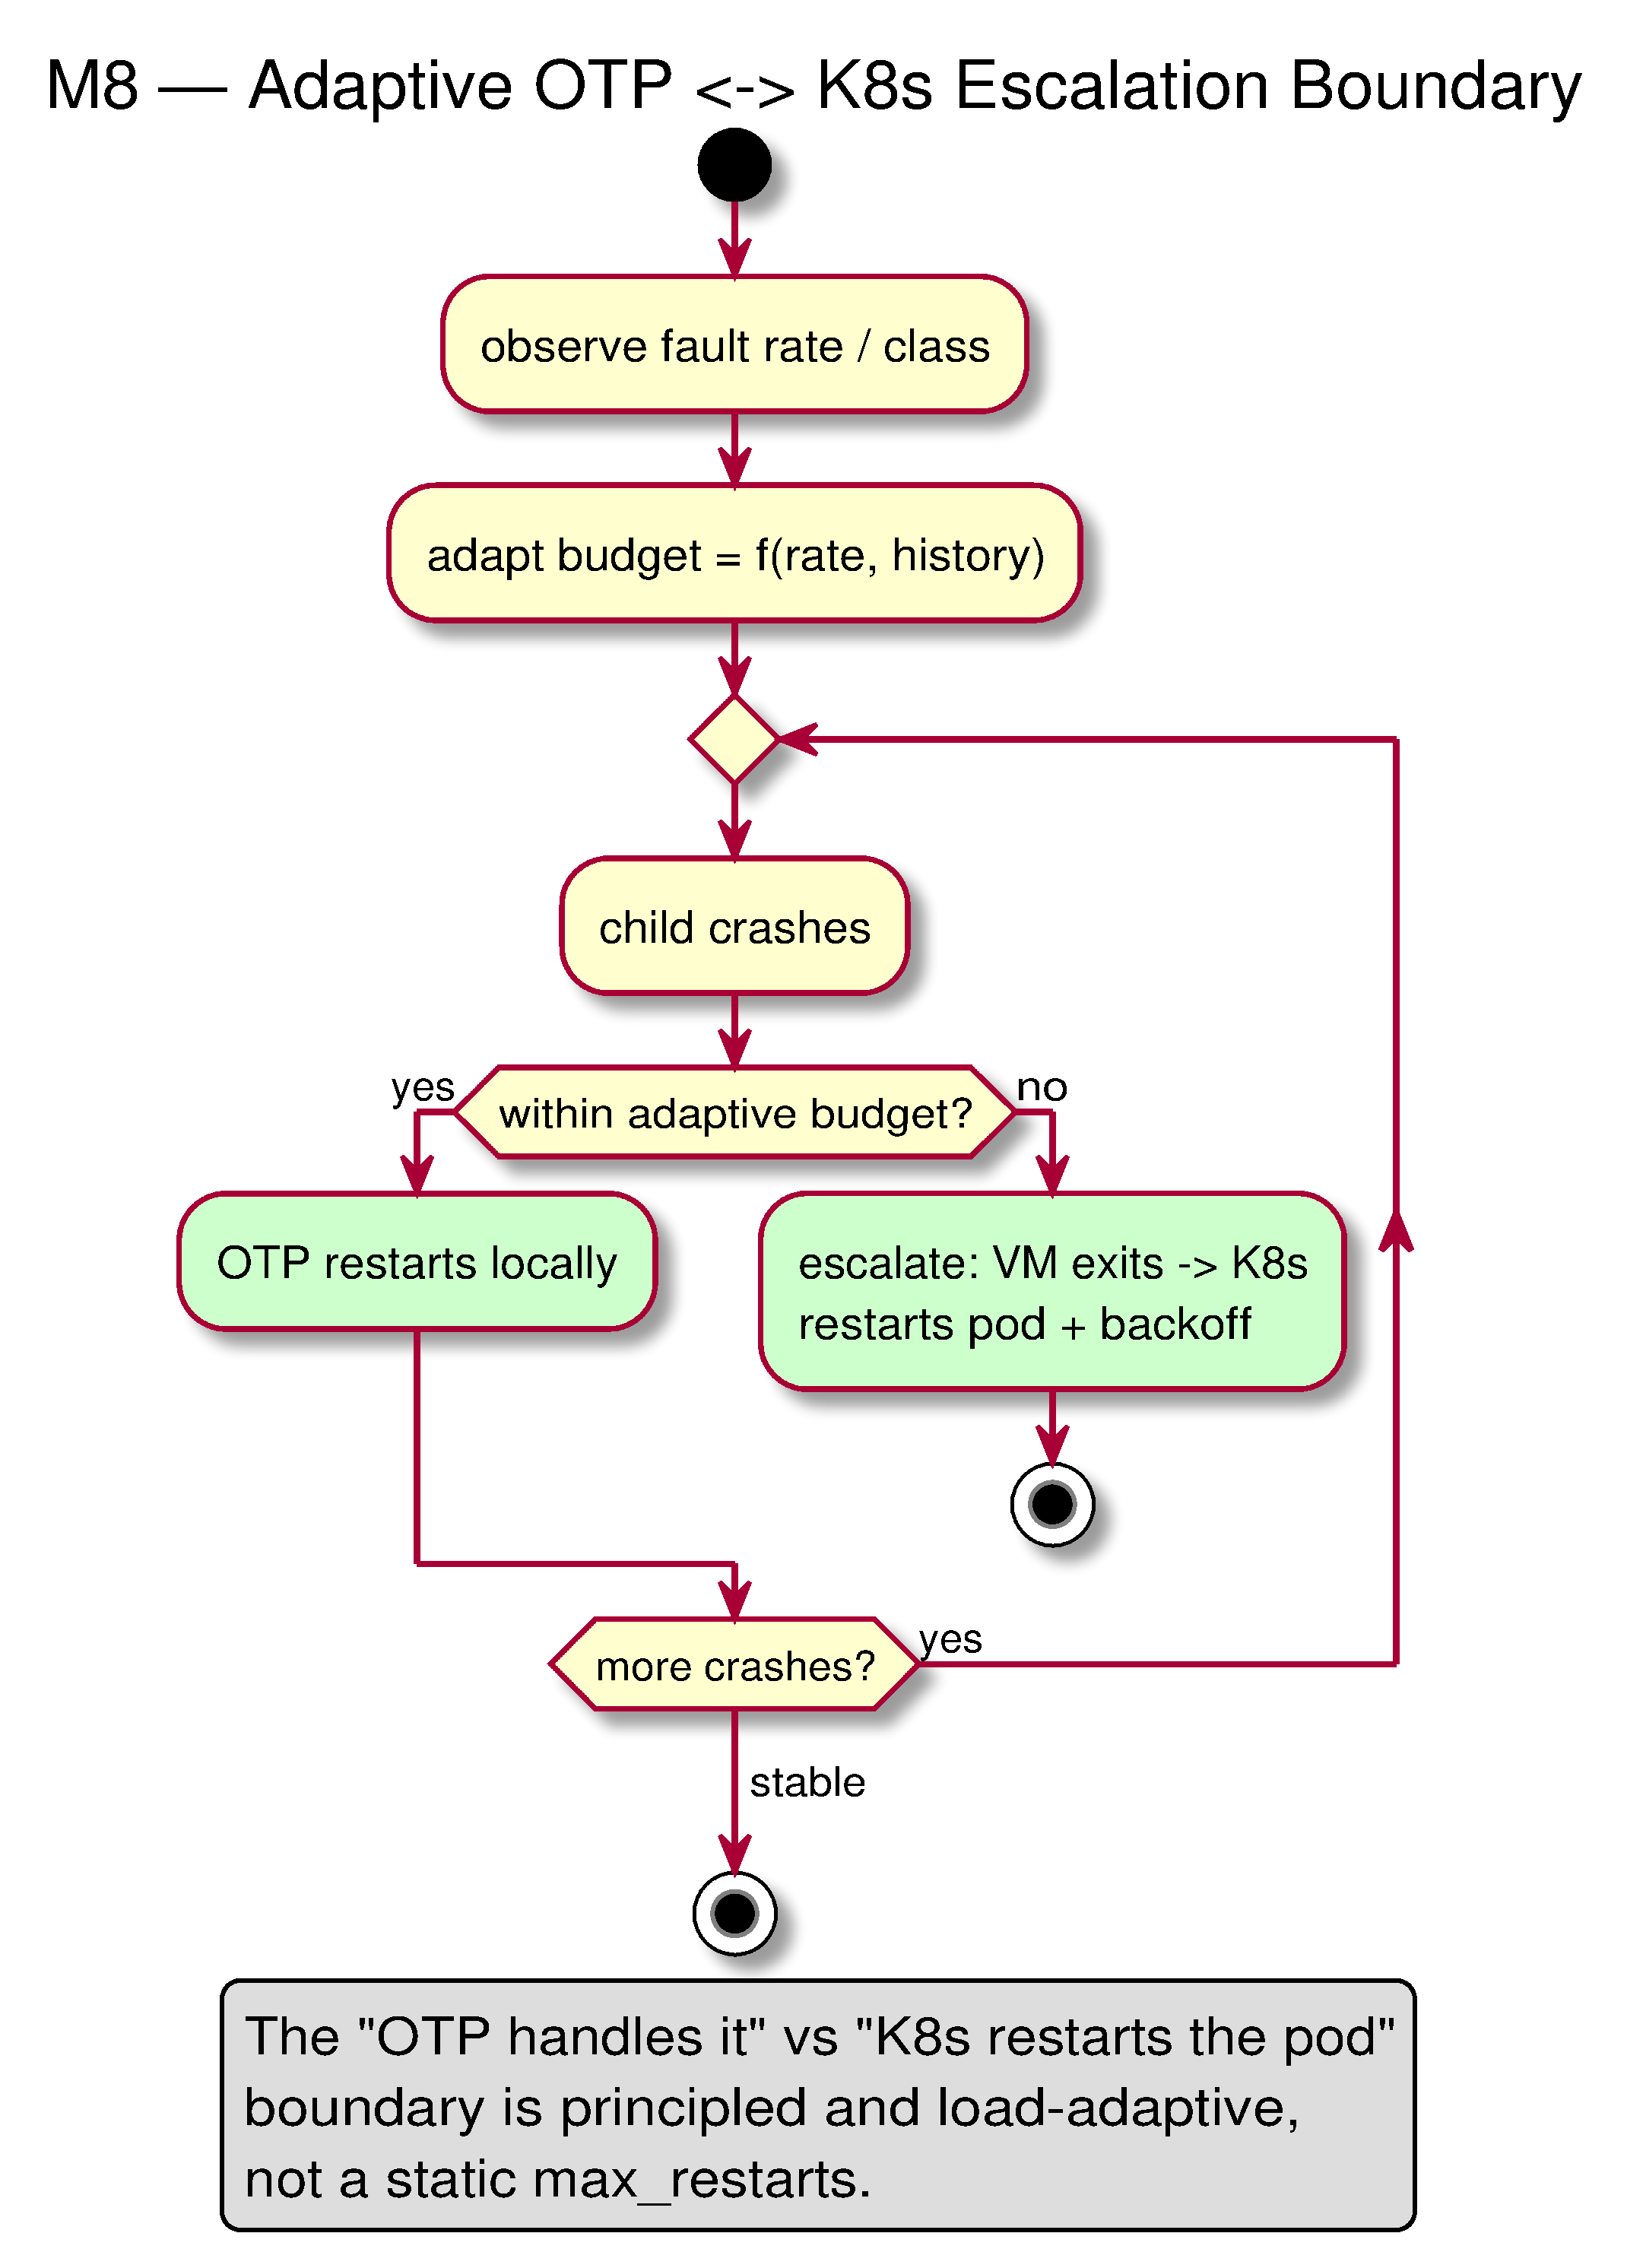
\includegraphics[width=\linewidth,height=0.9\textheight,keepaspectratio]{m8-adaptive-restart-budget-activity}
  \caption{M8 (aktivitas): batas ``OTP menangani'' vs.\ ``K8s me-\emph{restart pod}''
  ditetapkan secara adaptif terhadap beban, bukan konstanta statis.}\label{fig:m8-act}\end{figure}
\begin{algorithm}[H]\caption{M8 --- eskalasi \emph{restart-budget} adaptif.}\label{alg:m8}
\begin{algorithmic}[1]
\Loop
  \State $r \gets$ \Call{ObservedFaultRate}{}; $(M_r,M_s) \gets$ \Call{AdaptBudget}{$r$, \textit{hist}}
  \State \Call{OTP.SetRestartIntensity}{$M_r, M_s$}
\EndLoop
\State \textbf{on} \textsc{IntensityExceeded}: \Call{OTP.TerminateTree}{}; \Call{Exit}{$\neq 0$} \Comment{K8s backoff}
\end{algorithmic}\end{algorithm}

\noindent\textbf{Pembahasan.} Diagram sekuens (Gambar~\ref{fig:m8-seq}) menelusuri umpan
\emph{BEAM metrics}~$\rightarrow$~pengendali~$\rightarrow$~penyetelan jatah pada supervisor;
ketika jatah terlampaui, VM keluar dan Kubernetes me-\emph{restart} dengan \emph{backoff}.
Diagram aktivitas (Gambar~\ref{fig:m8-act}) menggambarkan perulangan ``\emph{crash} di
dalam jatah?''---ya: OTP menyalakan ulang; tidak: eskalasi. Algoritma~\ref{alg:m8}
memerincinya: \emph{loop} baris~1--4 mengamati \emph{fault rate} $r$, menghitung jatah baru
$(M_r,M_s)=f(r,\textit{hist})$, dan menyetelnya pada OTP; baris~5 menangani
\textsc{IntensityExceeded} dengan mematikan pohon dan keluar non-nol---batas eskalasi yang
terprinsip dan adaptif-beban.

\section{M9 --- Sinyal \emph{Liveness} Komposit BEAM}
\label{sec:m9}
Sebuah agregator menghitung kesehatan komposit dari utilisasi \emph{scheduler}, panjang
\emph{run-queue}, tekanan \emph{message-queue}, dan intensitas \emph{restart}---semuanya
metrik internal VM BEAM---menggantikan \emph{probe} TCP/HTTP.
\begin{figure}[H]\centering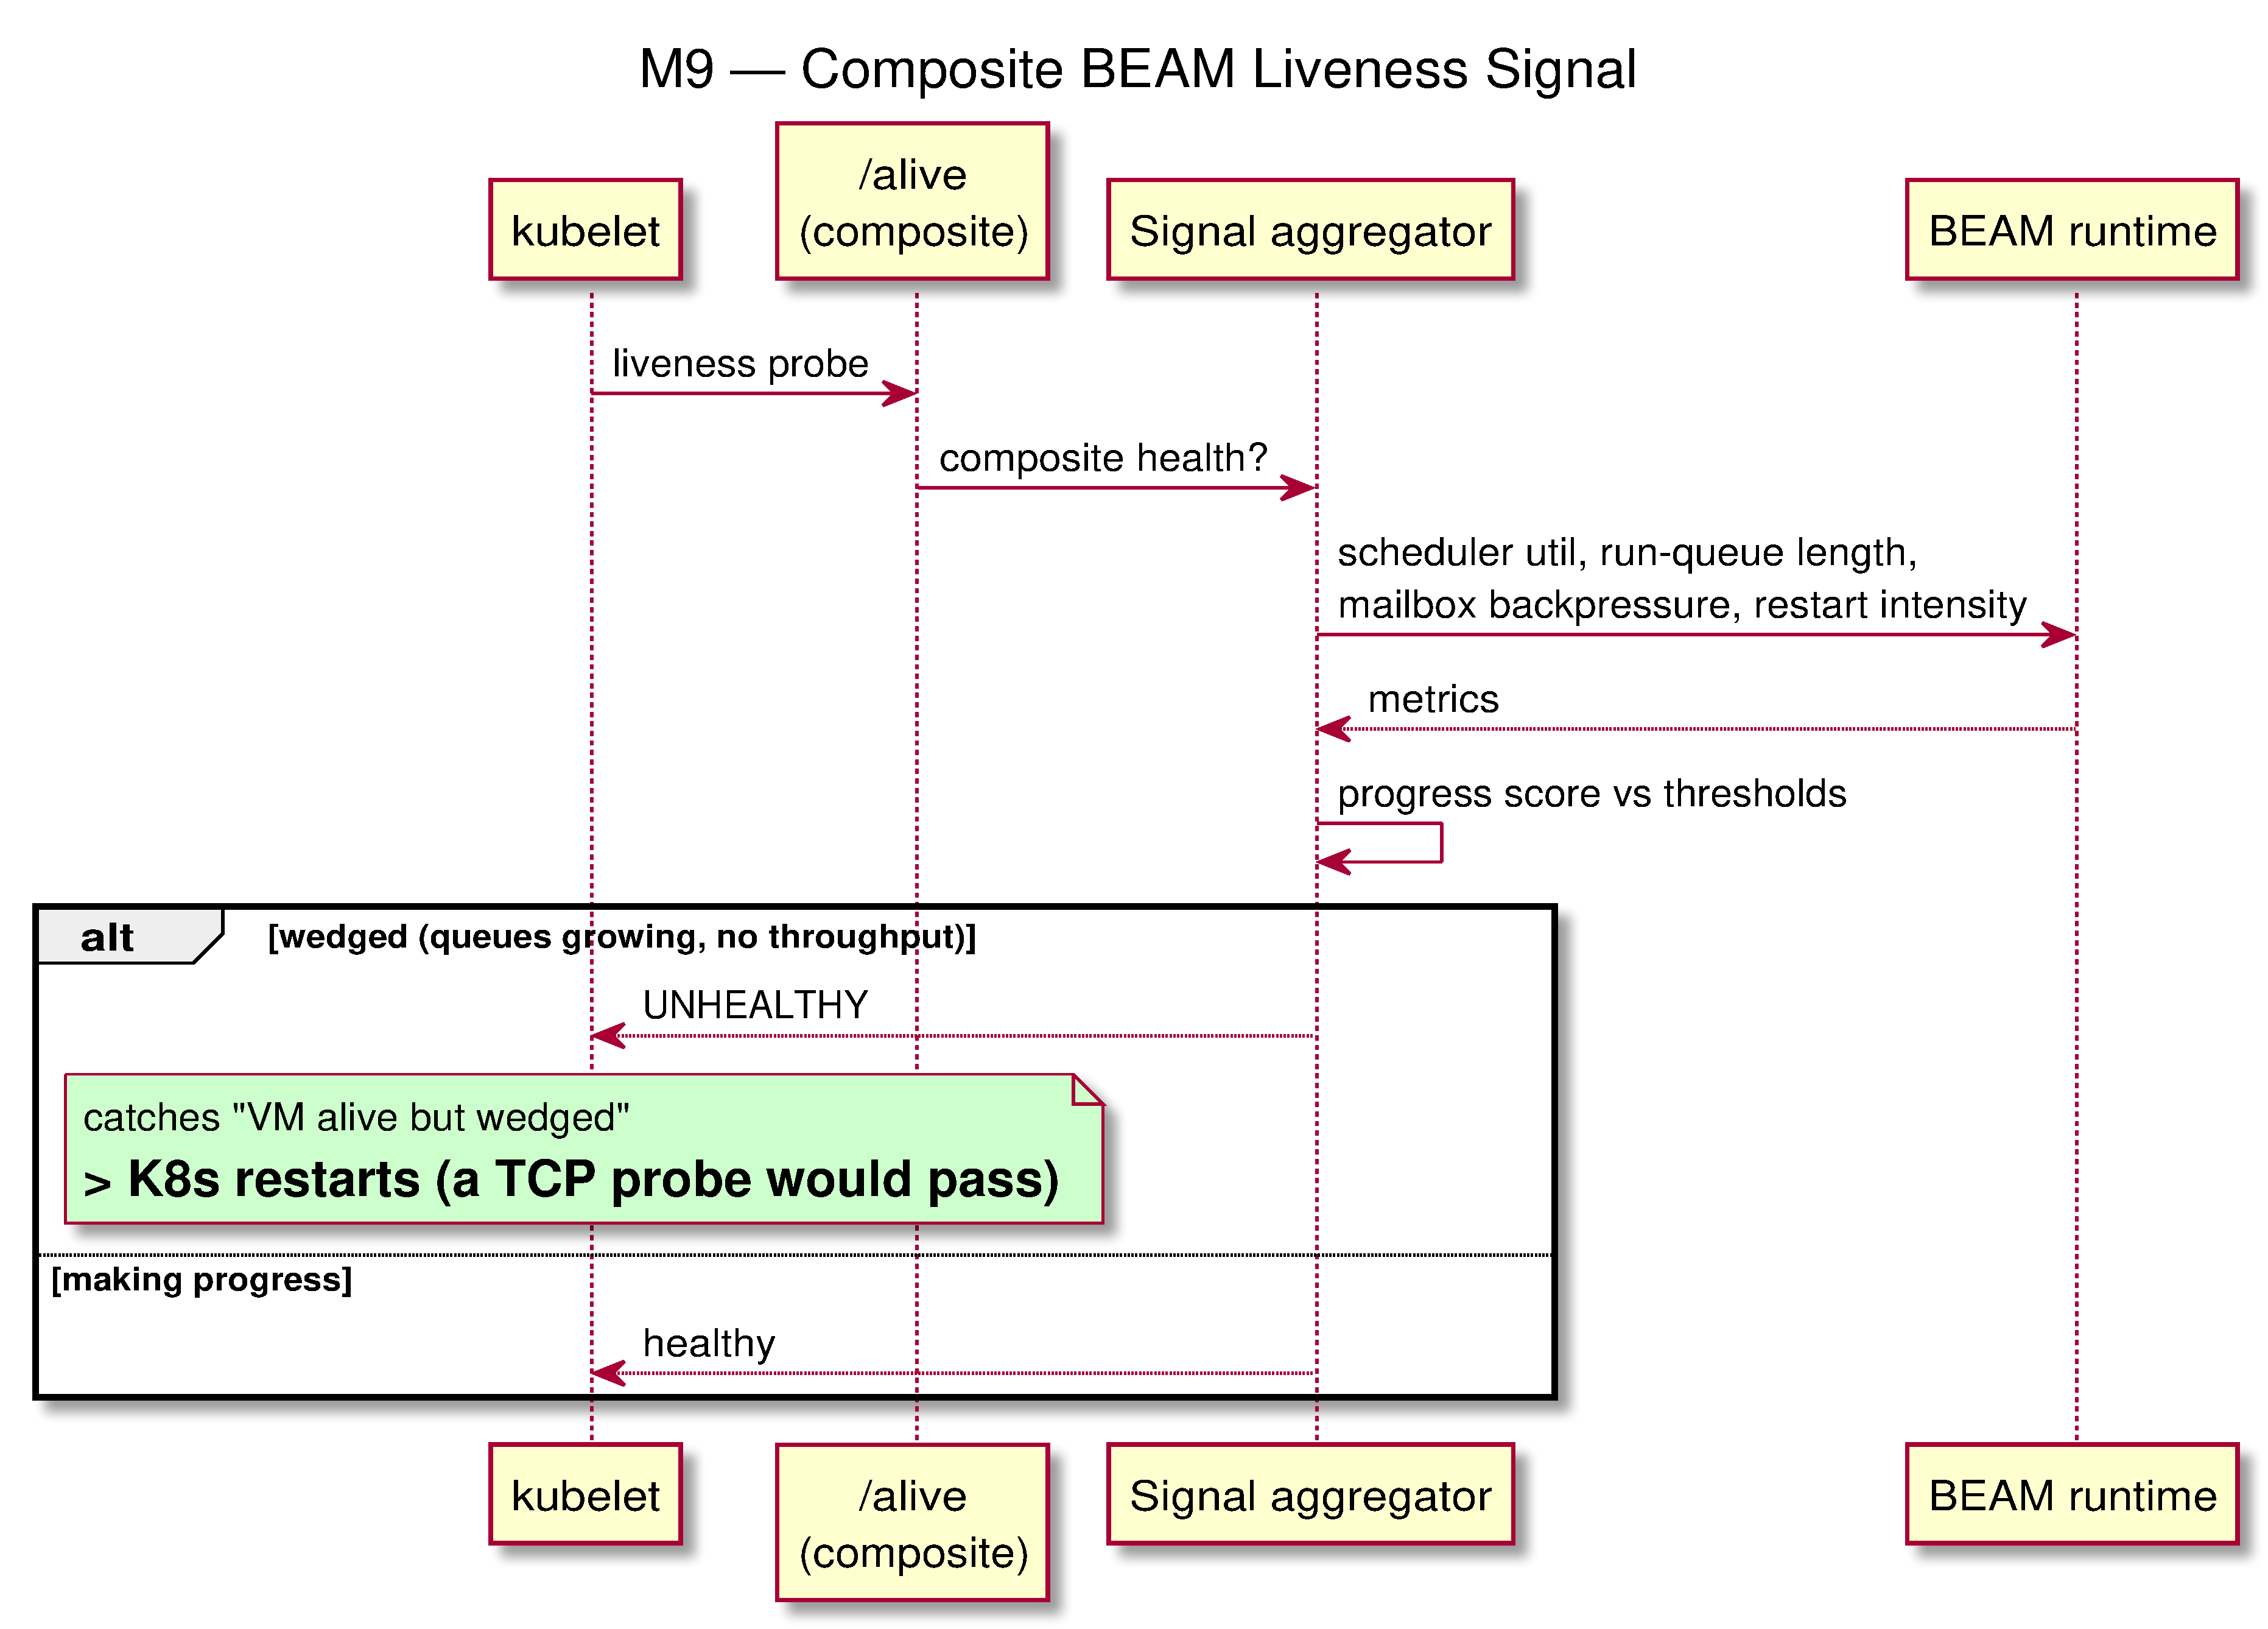
\includegraphics[width=\linewidth,height=0.9\textheight,keepaspectratio]{m9-composite-liveness-signal-sequence}
  \caption{M9 (sekuens): \emph{signal aggregator} mengumpulkan sinyal runtime BEAM dan
  melayani \texttt{/alive} komposit; macet terdeteksi meski VM ``hidup''.}\label{fig:m9-seq}\end{figure}
\begin{figure}[H]\centering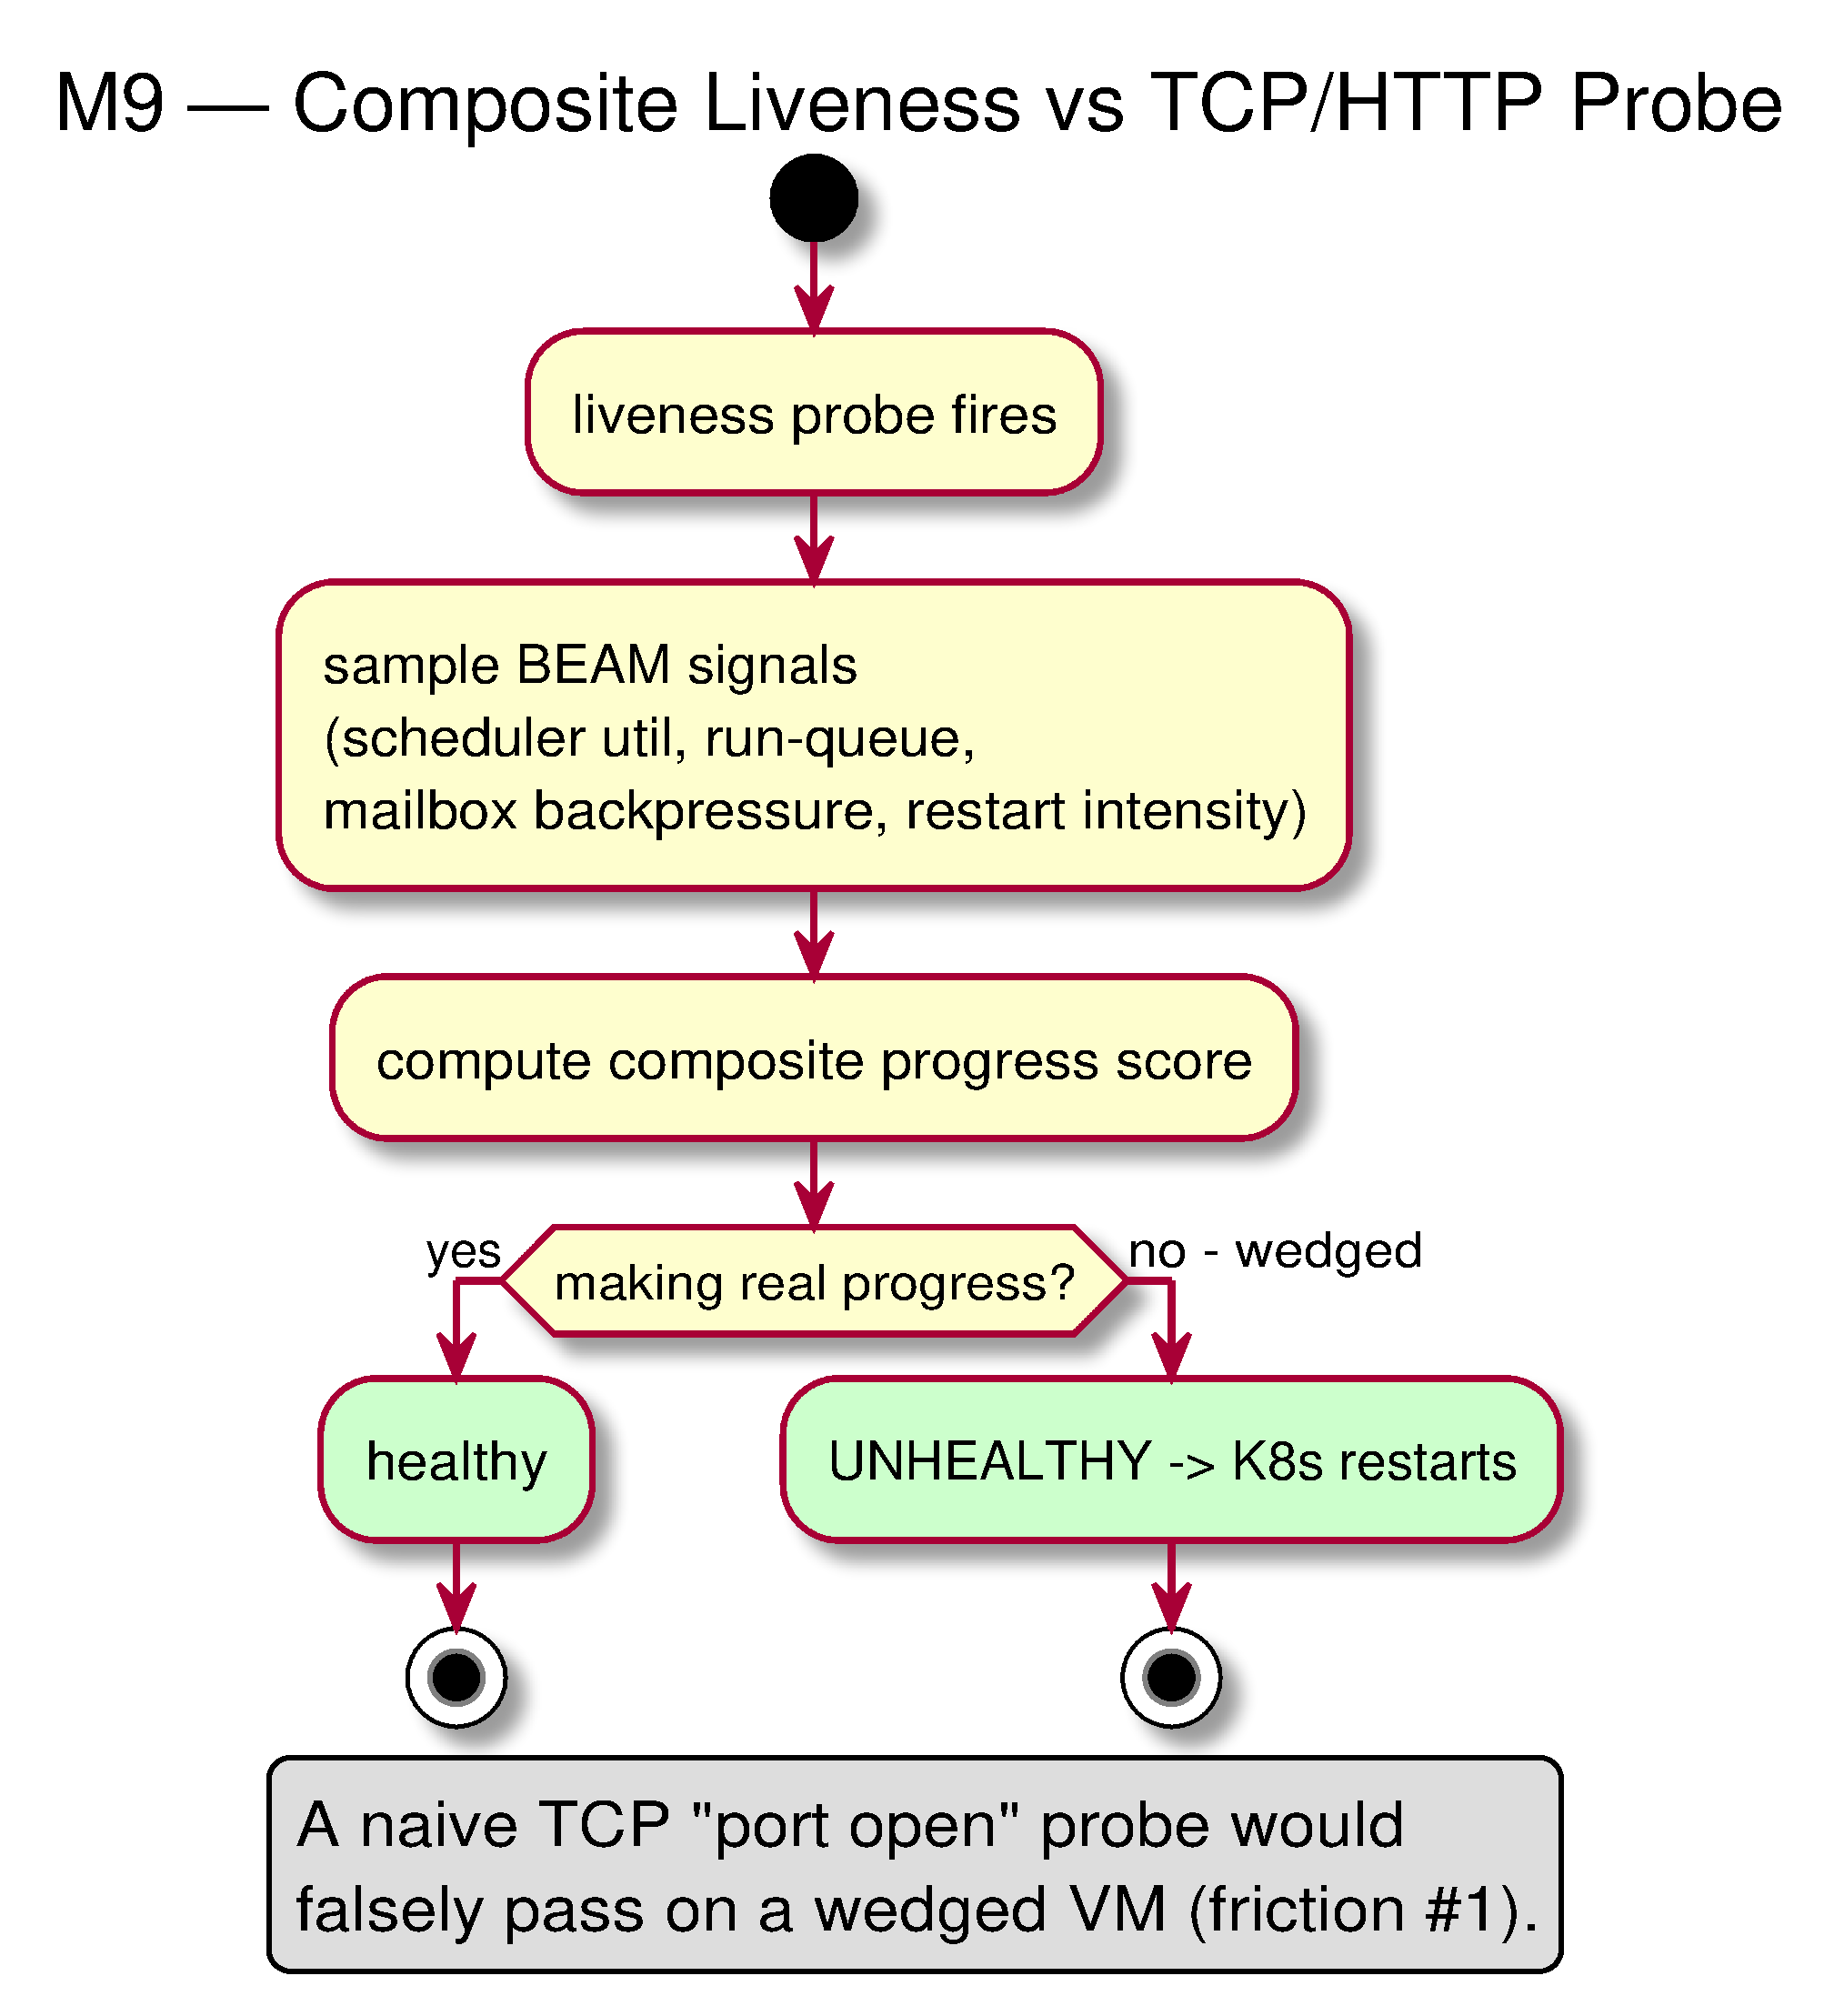
\includegraphics[width=\linewidth,height=0.9\textheight,keepaspectratio]{m9-composite-liveness-signal-activity}
  \caption{M9 (aktivitas): \emph{composite progress score} dibandingkan ambang; di bawah
  ambang berarti tidak sehat, menangkap kasus ``\emph{wedged VM}''.}\label{fig:m9-act}\end{figure}
\begin{algorithm}[H]\caption{M9 --- sinyal \emph{liveness} komposit BEAM.}\label{alg:m9}
\begin{algorithmic}[1]
\Function{LivenessHandler}{}
  \State $\sigma \gets (\textit{schedUtil}, \textit{runQueue}, \textit{mailbox}, \textit{restartRate})$
  \State $s \gets$ \Call{ProgressScore}{$\sigma$}
  \If{$s < \theta$} \State \Return \textit{unhealthy} \Else\ \State \Return \textit{healthy} \EndIf
\EndFunction
\end{algorithmic}\end{algorithm}

\noindent\textbf{Pembahasan.} Diagram sekuens (Gambar~\ref{fig:m9-seq}) menelusuri
kubelet~$\rightarrow$~\texttt{/alive}~$\rightarrow$~\emph{signal aggregator}~$\rightarrow$~runtime
BEAM, lalu skor dikembalikan---menangkap ``\emph{wedged VM}'' yang lolos pada Masalah~1.
Diagram aktivitas (Gambar~\ref{fig:m9-act}) menempatkan satu percabangan: ``skor kemajuan
$< \theta$?''. Algoritma~\ref{alg:m9} memerincinya: baris~2 mengumpulkan vektor sinyal
$\sigma$ (utilisasi \emph{scheduler}, panjang \emph{run-queue}, \emph{mailbox}, intensitas
\emph{restart}); baris~3 menghitung \emph{composite progress score} $s$; baris~4
mengembalikan \textit{unhealthy} bila $s<\theta$, selainnya \textit{healthy}---vonis yang
mencerminkan kemajuan nyata, bukan sekadar \emph{port} terbuka.


\chapter{Rancangan: Protokol Koordinasi Lintas-Lapis}
\label{ch:design}
Kontribusi inti memaketkan M3, M7, dan M8---ditambah bagian M4 yang baru bagi BEAM
(\emph{handoff-blocking termination} dan \emph{readiness} berbasis \emph{supervision
tree})---menjadi satu protokol koordinasi dengan kontrak kepemilikan/\emph{handoff} yang
jelas antara supervisor OTP dan pengendali Kubernetes.
\todo{mesin keadaan (\emph{state machine}); antarmuka OTP$\leftrightarrow$K8s; hukum
kendali (hukum \emph{grace} M3, pemetaan kuorum$\rightarrow$PDB M7, fungsi eskalasi
\emph{restart-budget}$\leftrightarrow$\emph{backoff} M8); invarian keselamatan: tanpa
pemulihan ganda, tanpa pelanggaran kuorum, tanpa \texttt{SIGKILL} di tengah \emph{handoff}.}

\chapter{Metodologi Evaluasi}
\label{ch:eval}
\textbf{Testbed.} Aplikasi Phoenix/Elixir dengan libcluster + Horde di atas \emph{cluster}
\texttt{kind}, dalam dua \emph{build}: terkoordinasi dan \emph{baseline} tanpa koordinasi.
\textbf{Kesalahan} (dipetakan ke Bab~\ref{ch:problems}): \emph{rolling deploy},
\emph{node drain}, partisi jaringan, OOM, subsistem macet, dan \emph{crash-loop}---disuntik
dengan Chaos Mesh / LitmusChaos. \textbf{Metrik:} MTTR, kehilangan permintaan/koneksi,
laju kehilangan state, jumlah \emph{restart} mubazir, dan \emph{overhead} koordinasi.
\todo{matriks eksperimen; jumlah ulangan $N$; uji statistik; hasil.}

\chapter{Diskusi}
\label{ch:disc}
\section{Generalisasi}
\todo{posisikan terhadap Akka~\cite{akkaHealth,akkaLease} dan Orleans~\cite{orleans};
asimetri lintas-platform; replikasi kecil di Akka untuk validitas eksternal.}
\section{Ancaman terhadap Validitas}
\todo{validitas konstruk/internal/eksternal/kesimpulan; bias satu ekosistem; realisme
injeksi kesalahan; keyakinan kebaruan masih sedang sebelum verifikasi ulang.}

\chapter{Kesimpulan}
\label{ch:conclusion}
\todo{nyatakan ulang celah koordinasi, protokol yang diusulkan, hasil utama, dan
generalisasinya.}

\bibliographystyle{plain}
\bibliography{refs}

\appendix
% glossary.tex — \input dari report.tex (lampiran)
\chapter{Daftar Istilah}
\label{ch:glosarium}

Lampiran ini menjelaskan istilah-istilah teknis yang dipakai di laporan, disertai
contoh singkat. Istilah teknis sengaja dipertahankan dalam bahasa aslinya karena itulah
bentuk yang lazim dipakai praktisi. Daftar ini panjang karena topiknya menjembatani dua
ekosistem (BEAM/Elixir dan Kubernetes)---namun \textbf{pembaca tidak perlu menghafal
semuanya}: cukup pahami dua belas istilah inti pada Tabel~\ref{tab:inti}, sisanya bersifat
rujukan saat diperlukan.

\section*{Peta Cepat: Istilah Inti}
\begin{table}[H]\centering\small
\caption{Dua belas istilah inti yang cukup untuk mengikuti alur laporan.}
\label{tab:inti}
\begin{tabular}{@{}p{0.30\linewidth}p{0.62\linewidth}@{}}
\toprule
\textbf{Istilah} & \textbf{Inti} \\
\midrule
BEAM & VM Erlang tempat Elixir berjalan. \\
OTP / \emph{supervision tree} & Pola supervisi yang menyalakan ulang \emph{process} yang gagal. \\
libcluster & Pembentukan \emph{cluster} BEAM otomatis di Kubernetes. \\
Horde & \emph{Supervisor}/\emph{registry} terdistribusi dengan \emph{handoff}. \\
Handoff & Pemindahan \emph{process} beserta \emph{state} ke node lain. \\
Split-brain & Partisi jaringan yang membuat dua sisi \emph{cluster} sama-sama aktif. \\
Probe (\emph{liveness}/\emph{readiness}) & Pemeriksaan kesehatan oleh Kubernetes. \\
Grace period & Tenggat antara \texttt{SIGTERM} dan \texttt{SIGKILL}. \\
PDB & Batas \emph{pod} yang boleh \emph{down} saat gangguan sukarela. \\
Operator (Bonny) & Pengendali kustom Kubernetes, ditulis dalam Elixir. \\
Kubernetes Lease & Objek koordinasi/\emph{fencing} berbasis etcd. \\
Kuorum BEAM & Jumlah node minimum agar \emph{cluster} otoritatif. \\
\bottomrule
\end{tabular}
\end{table}

\section{Ekosistem BEAM / Elixir}
\begin{description}[style=nextline,leftmargin=1.4em]
  \item[BEAM] Mesin virtual Erlang tempat Elixir dijalankan; menjalankan jutaan
    \emph{process} ringan terisolasi. \emph{Contoh:} aplikasi Phoenix berjalan sebagai
    satu instans BEAM dalam satu \emph{pod}.
  \item[OTP] Pustaka dan pola Erlang (\emph{supervisor}, \texttt{GenServer}) untuk sistem
    tahan-gagal. \emph{Contoh:} \emph{supervisor} OTP menyalakan ulang pekerja yang \emph{crash}.
  \item[Supervision tree] Hierarki \emph{supervisor}--anak yang menentukan pola pemulihan.
    \emph{Contoh:} lihat Listing~\ref{lst:sup}.
  \item[Supervisor] \emph{Process} yang memantau dan menyalakan ulang anak menurut
    strategi (\texttt{:one\_for\_one}, dll). \emph{Contoh:} memulai ulang hanya anak yang gagal.
  \item[GenServer] Abstraksi \emph{process} \emph{stateful}. \emph{Contoh:} satu sesi
    dokumen direpresentasikan sebagai satu \texttt{GenServer}.
  \item[Process (BEAM)] Unit eksekusi ringan BEAM, bukan \emph{process} OS.
    \emph{Contoh:} ratusan ribu \emph{process} dalam satu VM.
  \item[Let it crash] Filosofi membiarkan \emph{process} gagal lalu dipulihkan supervisor.
    \emph{Contoh:} tidak menulis \emph{defensive code}, cukup biarkan \emph{crash} dan restart.
  \item[Restart] Penyalaan ulang \emph{process} oleh supervisor setelah \emph{crash}.
    \emph{Contoh:} \emph{decoder} yang \emph{crash} disalakan ulang otomatis.
  \item[Restart-budget] Batas intensitas \emph{restart} (\texttt{max\_restarts} dalam
    \texttt{max\_seconds}); bila terlampaui, supervisor menyerah dan tereskalasi ke induk.
    \emph{Contoh:} \texttt{3} \emph{restart} dalam \texttt{5} detik.
  \item[libcluster] Pembentukan \emph{cluster} BEAM otomatis di Kubernetes. \emph{Contoh:}
    strategi \texttt{Kubernetes.DNS} menemukan \emph{peer} lewat \emph{headless service}.
  \item[Horde] \emph{Supervisor}/\emph{registry} terdistribusi berbasis CRDT dengan
    \emph{handoff}. \emph{Contoh:} memindahkan \emph{process} ke node tersisa saat node hilang.
  \item[Handoff] Pemindahan \emph{process} beserta \emph{state}-nya ke node lain.
    \emph{Contoh:} Horde memindahkan \emph{process} dokumen sebelum \emph{pod} mati.
  \item[Phoenix] Kerangka kerja web Elixir. \emph{Contoh:} \emph{endpoint} HTTP pada \emph{port} 4000.
  \item[\texttt{:global}] \emph{Registry} nama global lintas-node bawaan Erlang.
    \emph{Contoh:} mendaftarkan \emph{singleton} agar unik di seluruh \emph{cluster}.
  \item[CRDT] \emph{Conflict-free Replicated Data Type}---konvergen tanpa koordinasi.
    \emph{Contoh:} Horde memakai \texttt{DeltaCrdt}.
  \item[Erlang distribution cookie] Rahasia bersama yang harus seragam antar-node.
    \emph{Contoh:} disuntikkan via \emph{Secret} Kubernetes.
  \item[Kuorum BEAM] Jumlah node minimum agar satu sisi \emph{cluster} dianggap otoritatif
    (mayoritas). \emph{Contoh:} \texttt{Horde.UniformQuorumDistribution} mematikan sisi
    dengan kurang dari setengah node.
\end{description}

\section{Kubernetes}
\begin{description}[style=nextline,leftmargin=1.4em]
  \item[Kubernetes] Orkestrator kontainer yang menjadwalkan, memantau, dan memulihkan
    beban kerja. \emph{Contoh:} me-\emph{restart pod} yang gagal \emph{probe}.
  \item[Control plane] Otak Kubernetes (API \emph{server}, \emph{scheduler}, \emph{controller}).
    \emph{Contoh:} menyimpan keadaan ke etcd.
  \item[etcd] Penyimpanan \emph{key-value} konsisten (Raft), \emph{backend control plane}.
    \emph{Contoh:} mendukung penguncian \emph{Lease}.
  \item[Pod] Unit penyebaran terkecil (satu/lebih kontainer). \emph{Contoh:} satu \emph{pod}
    memuat satu instans BEAM.
  \item[Node] Mesin (fisik/VM) anggota \emph{cluster}. \emph{Contoh:} \emph{pod}
    dijadwalkan ulang ke node sehat saat node-nya mati.
  \item[kubelet] Agen Kubernetes di tiap node yang menjalankan \emph{probe} dan mengelola
    siklus hidup \emph{pod}. \emph{Contoh:} kubelet mengirim \texttt{SIGTERM} saat \emph{pod} diterminasi.
  \item[Probe] Pemeriksaan kesehatan berkala oleh kubelet (\emph{liveness}/\emph{readiness}/\emph{startup}).
    \emph{Contoh:} \texttt{HTTP GET /healthz}.
  \item[Liveness probe] ``Apakah kontainer hidup?''; gagal $\rightarrow$ di-\emph{restart}.
    \emph{Contoh:} memeriksa \emph{port} 4000.
  \item[Readiness] Keadaan ``siap menerima lalu lintas''; \emph{readiness probe} mengatur
    keanggotaan \emph{endpoint Service}. \emph{Contoh:} \texttt{/readyz} mengembalikan 503
    sampai \emph{cluster} terbentuk.
  \item[Startup probe] \emph{Probe} untuk boot lambat sebelum \emph{liveness} aktif.
    \emph{Contoh:} menunggu migrasi basis data.
  \item[failureThreshold] Jumlah kegagalan \emph{probe} berturut-turut sebelum kontainer
    dianggap gagal. \emph{Contoh:} \texttt{failureThreshold: 1} membunuh \emph{pod} setelah
    satu kegagalan (positif palsu pada Masalah~1).
  \item[Readiness gate] Kondisi \emph{pod} kustom tambahan yang memengaruhi \emph{readiness}.
    \emph{Contoh:} siap hanya bila anggota \emph{cluster} BEAM \texttt{Up}.
  \item[SIGTERM] Sinyal terminasi sopan yang dikirim sebelum penghentian paksa.
    \emph{Contoh:} memicu \emph{drain} dan \emph{handoff}.
  \item[SIGKILL] Sinyal penghentian paksa setelah \emph{grace period} habis (tak dapat
    ditangkap). \emph{Contoh:} membunuh \emph{process} yang belum selesai \emph{handoff}.
  \item[Graceful shutdown] Mematikan tertib: berhenti menerima koneksi, \emph{drain},
    \emph{handoff}, lalu berhenti. \emph{Contoh:} menyelesaikan permintaan yang sedang berjalan.
  \item[terminationGracePeriodSeconds (grace period)] Tenggat antara \texttt{SIGTERM} dan
    \texttt{SIGKILL}. \emph{Contoh:} \texttt{30} detik.
  \item[preStop hook] Perintah/HTTP sebelum \texttt{SIGTERM}. \emph{Contoh:} tidur sejenak
    agar penghapusan \emph{endpoint} merambat.
  \item[Blocking termination] Menahan penghapusan \emph{pod} (mis.\ via \emph{finalizer})
    hingga syarat terpenuhi. \emph{Contoh:} menunda terminasi sampai \emph{handoff} Horde selesai.
  \item[Drain / eviction] Pengosongan \emph{pod} dari node (gangguan sukarela).
    \emph{Contoh:} \texttt{kubectl drain} saat pemeliharaan.
  \item[Rolling update] Pembaruan bertahap yang mengganti \emph{pod} sedikit demi sedikit.
    \emph{Contoh:} mengganti \emph{image} versi baru tanpa \emph{downtime}.
  \item[PodDisruptionBudget (PDB)] Batas \emph{pod} yang boleh tidak tersedia saat gangguan
    sukarela. \emph{Contoh:} \texttt{minAvailable: 2}.
  \item[maxUnavailable] Jumlah/persentase \emph{pod} maksimum yang boleh tidak tersedia saat
    \emph{rolling update}/PDB. \emph{Contoh:} \texttt{maxUnavailable: 1}.
  \item[anti-affinity] Aturan penjadwalan agar \emph{pod} tidak ditempatkan berdekatan
    (mis.\ node sama). \emph{Contoh:} menyebar replika antar-node demi ketahanan.
  \item[backoff] Penundaan yang meningkat antar-percobaan \emph{restart}
    (\texttt{CrashLoopBackOff}). \emph{Contoh:} jeda kian lama saat \emph{pod} terus gagal.
  \item[Operator / Controller / CRD] Pengendali kustom yang merekonsiliasi \emph{Custom
    Resource}. \emph{Contoh:} operator menyediakan basis data per-penyewa.
  \item[Bonny] Kerangka menulis \emph{operator} Kubernetes dalam Elixir. \emph{Contoh:}
    mengawasi CRD dan merekonsiliasi keadaan.
  \item[Kubernetes Lease] Objek koordinasi (\texttt{kind: Lease}) didukung etcd untuk
    penguncian/\emph{leader election}/\emph{fencing}. \emph{Contoh:} Akka memakainya sebagai
    arbiter \emph{split-brain}~\cite{akkaLease}.
  \item[KEDA / HPA] Penskala otomatis berbasis metrik/event (KEDA) dan sumber daya (HPA).
    \emph{Contoh:} KEDA menskala dari panjang antrian Oban.
\end{description}

\section{Konsep, Evaluasi, dan Platform Lain}
\begin{description}[style=nextline,leftmargin=1.4em]
  \item[Chaos Mesh] Perkakas \emph{chaos engineering} Kubernetes. \emph{Contoh:}
    \texttt{NetworkChaos} membuat partisi; \texttt{PodChaos} mematikan \emph{pod}.
  \item[LitmusChaos] Kerangka \emph{chaos engineering} Kubernetes berbasis eksperimen.
    \emph{Contoh:} eksperimen \texttt{pod-delete}.
  \item[Fault injection] Penyuntikan kesalahan terkendali untuk menguji ketahanan.
    \emph{Contoh:} mematikan node saat beban penuh.
  \item[MAPE-K] \emph{Loop} otonomik \emph{Monitor-Analyze-Plan-Execute} di atas
    \emph{Knowledge}. \emph{Contoh:} operator sebagai \emph{self-healing loop}.
  \item[Split-brain] Partisi jaringan yang membuat dua sisi \emph{cluster} sama-sama aktif.
    \emph{Contoh:} dua sisi mendaftarkan \emph{singleton} yang sama.
  \item[Fencing] Mencegah sisi yang tidak otoritatif terus bertindak.
    \emph{Contoh:} hanya pemegang \emph{Lease} yang boleh bertahan.
  \item[Arbiter] Pihak eksternal yang memutuskan sisi mana yang otoritatif saat
    konflik/partisi. \emph{Contoh:} \emph{Kubernetes Lease} (etcd) menjadi \emph{arbiter}
    \emph{split-brain} pada M5.
  \item[Double recovery] Dua lapis memulihkan satu kegagalan secara mubazir.
    \emph{Contoh:} OTP me-\emph{restart} \emph{process} sembari K8s me-\emph{restart pod}.
  \item[Drift (konfigurasi)] Divergensi pengaturan antar sumber/lapis yang seharusnya
    konsisten. \emph{Contoh:} \emph{probe} K8s dan \texttt{max\_restarts} OTP tak sinkron.
  \item[MTTR] \emph{Mean Time To Recovery}---rerata waktu pulih. \emph{Contoh:} metrik
    utama evaluasi (Bab~\ref{ch:eval}).
  \item[kind] \emph{Kubernetes IN Docker}---\emph{cluster} lokal untuk pengujian.
    \emph{Contoh:} \emph{testbed} evaluasi.
  \item[Akka / Orleans] \emph{Toolkit actor} JVM (Akka) dan kerangka \emph{virtual actor}
    .NET (Orleans). \emph{Contoh:} Akka memantulkan keanggotaan \emph{cluster} ke
    \emph{readiness}~\cite{akkaHealth}.
\end{description}

\section{Istilah pada Diagram (Sekuens/Aktivitas)}
Istilah-istilah berikut muncul pada label dan catatan di dalam diagram.
\begin{description}[style=nextline,leftmargin=1.4em]
  \item[Cowboy / Bandit] Server HTTP untuk BEAM yang dipakai Phoenix. \emph{Contoh:}
    Cowboy menerima koneksi TCP di \emph{port} 4000.
  \item[Finch] Klien HTTP berbasis \emph{pool} koneksi. \emph{Contoh:} \emph{pool} Finch
    memanggil API \emph{fraud} eksternal pada \emph{PayGate}.
  \item[Ecto] Pustaka basis data Elixir dengan \emph{pool} koneksi. \emph{Contoh:}
    \emph{pool} Ecto menyambung ulang saat \emph{failover} basis data.
  \item[MatchError] Galat Elixir saat pencocokan pola gagal. \emph{Contoh:} \emph{frame}
    cacat memicu \texttt{MatchError} pada \emph{decoder}.
  \item[\texttt{:one\_for\_one}] Strategi supervisi: hanya anak yang gagal yang disalakan
    ulang. \emph{Contoh:} lihat Listing~\ref{lst:sup}.
  \item[EXIT] Sinyal yang dikirim saat \emph{process} berhenti/\emph{crash}, ditangkap
    supervisor. \emph{Contoh:} \emph{decoder} mengirim \texttt{EXIT} ke supervisornya.
  \item[nodedown] Peristiwa saat sebuah node distribusi terputus. \emph{Contoh:} saat
    partisi, tiap sisi melihat sisi lain \texttt{nodedown}.
  \item[Wedged (macet)] \emph{Process} yang hidup tetapi tak membuat kemajuan (mis.\
    terblokir tanpa \emph{timeout}). \emph{Contoh:} pekerja \emph{pool} terblokir pada
    koneksi yang menggantung.
  \item[Wedged VM] Instans BEAM yang \emph{process} OS-nya hidup tetapi tak melayani
    permintaan karena subsistem kritis terblokir. \emph{Contoh:} \emph{probe} TCP lulus
    padahal 100\% pembayaran macet (negatif palsu pada M1/M9).
  \item[Naive TCP probe] \emph{Probe} yang hanya memeriksa apakah \emph{port} menerima
    koneksi TCP, tanpa menilai kesehatan aplikasi sebenarnya. \emph{Contoh:}
    \texttt{tcpSocket: 4000} lulus meski seluruh pekerja \emph{pool} macet.
  \item[Scheduler / utilisasi scheduler] Penjadwal BEAM yang menjalankan \emph{process};
    utilisasinya menandakan beban nyata. \emph{Contoh:} salah satu sinyal M9.
  \item[Run-queue] Antrian \emph{process} siap-jalan per \emph{scheduler}; yang membengkak
    menandakan kemacetan. \emph{Contoh:} indikator kesehatan pada M9.
  \item[Mailbox / message-queue backpressure] Antrian pesan tiap \emph{process}; backlog
    yang tumbuh menandakan \emph{backpressure}. \emph{Contoh:} \emph{mailbox} membengkak
    saat \emph{process} tak mengimbangi laju pesan.
  \item[Restart intensity] Laju \emph{restart} anak oleh supervisor; lonjakannya menandakan
    kegagalan berulang. \emph{Contoh:} dipakai M1 dan M9.
  \item[Deroute] Mengeluarkan \emph{pod} dari \emph{Service Endpoints} sehingga lalu lintas
    berhenti diarahkan ke sana (tanpa \emph{restart}). \emph{Contoh:} \emph{readiness} gagal
    $\rightarrow$ \emph{pod} di-\emph{deroute}.
  \item[Per-subtree restart intensity] Intensitas \emph{restart} dihitung per subpohon
    supervisi, bukan secara global. \emph{Contoh:} M1 memeriksa tiap subpohon.
  \item[Wedged-child detection] Deteksi anak supervisi yang hidup tetapi macet.
    \emph{Contoh:} dasar vonis tidak-sehat pada M1/M9.
  \item[Critical subtree] Subpohon supervisi yang menjalankan fungsi penting;
    kemacetan/over-\emph{restart}-nya menentukan vonis \emph{probe}. \emph{Contoh:} M1.
  \item[Up/down (status anak)] Keadaan anak supervisi hidup (\emph{up}) atau mati
    (\emph{down}). \emph{Contoh:} dimasukkan ke perhitungan kesehatan M1.
  \item[\texttt{/healthz} (derived)] \emph{Endpoint} \emph{healthz} yang vonisnya diturunkan
    dari keadaan \emph{supervision tree} (M1), bukan pemeriksaan dangkal, sehingga Kubernetes
    bertindak (\emph{deroute}/\emph{restart}) atas kesehatan supervisi yang sebenarnya.
  \item[Health deriver] Komponen M1 yang memeriksa \emph{OTP supervision tree} dan menghitung
    vonis \emph{probe}. \emph{Contoh:} memetakan intensitas \emph{restart}/kemacetan subpohon
    menjadi balasan 200 atau 503.
  \item[Fault rate] Laju kegagalan teramati per satuan waktu, menjadi masukan adaptasi M8.
    \emph{Contoh:} lonjakan \emph{crash} \emph{decoder} menaikkan \emph{fault rate}.
  \item[Adaptive budget] Penyetelan dinamis jatah \emph{restart}
    (\texttt{max\_restarts}/\texttt{max\_seconds}) menurut kondisi, bukan nilai statis.
    \emph{Contoh:} jatah diperketat saat \emph{fault rate} tinggi.
  \item[\texttt{f(rate, history)}] Fungsi adaptasi yang memetakan \emph{fault rate} dan
    riwayat ke jatah \emph{restart} baru. \emph{Contoh:} inti \textsc{AdaptBudget} pada
    Algoritma~\ref{alg:m8}.
  \item[Child crash] Peristiwa anak supervisor berhenti tak normal. \emph{Contoh:} memicu
    evaluasi apakah masih dalam jatah \emph{restart}.
  \item[Escalate (eskalasi)] Menyerahkan kegagalan ke lapis di atas
    (anak~$\rightarrow$~supervisor~$\rightarrow$~VM~$\rightarrow$~Kubernetes). \emph{Contoh:}
    jatah habis $\Rightarrow$ VM keluar $\Rightarrow$ K8s me-\emph{restart pod}.
  \item[Boundary (batas kepemilikan)] Ambang yang memisahkan ``OTP menangani'' dari ``K8s
    me-\emph{restart pod}''. \emph{Contoh:} ditetapkan secara adaptif oleh M8.
  \item[Principled \& load-adaptive] Sifat batas eskalasi: berlandas prinsip/terukur dan
    menyesuaikan beban, bukan konstanta sembarang. \emph{Contoh:} batas OTP$\leftrightarrow$K8s pada M8.
  \item[Signal aggregator] Komponen M9 yang merangkum sinyal runtime BEAM menjadi satu
    skor. \emph{Contoh:} menggabungkan \emph{scheduler}, \emph{run-queue}, dan \emph{mailbox}.
  \item[Sinyal liveness komposit BEAM] Sinyal kesehatan M9 yang menggabungkan beberapa
    metrik runtime BEAM (\emph{scheduler}, \emph{run-queue}, \emph{mailbox}, \emph{restart
    intensity}) menjadi satu vonis \emph{liveness}, menggantikan \emph{probe} TCP/HTTP.
    \emph{Contoh:} keluaran \emph{signal aggregator} pada \texttt{/alive}.
  \item[Composite progress score] Skor kesehatan gabungan dari beberapa sinyal; di bawah
    ambang berarti tidak sehat. \emph{Contoh:} keluaran \emph{signal aggregator} M9.
  \item[/alive (composite)] \emph{Endpoint} \emph{liveness} yang melayani skor komposit,
    bukan sekadar \emph{probe} TCP. \emph{Contoh:} dipakai M9 menggantikan \emph{probe} naif.
  \item[\texttt{terminate/2}, \texttt{handle\_continue/2}] \emph{Callback} OTP untuk
    menyimpan \emph{state} saat berhenti dan memulihkannya setelah inisialisasi.
    \emph{Contoh:} \emph{handoff} Horde menyimpan \emph{state} via \texttt{terminate/2}.
  \item[Phoenix.PubSub] \emph{Pub/sub} terdistribusi lintas-node. \emph{Contoh:} menyiarkan
    pesan ke semua pengguna antar-\emph{pod}.
  \item[Service / Endpoints] Abstraksi K8s yang merutekan lalu lintas ke \emph{pod} siap;
    daftar \emph{Endpoints} berisi \emph{pod} anggota. \emph{Contoh:} \emph{pod} ditambahkan
    ke \emph{Endpoints} saat \emph{ready}.
  \item[Deployment / ReplicaSet] Pengendali K8s yang menjaga jumlah replika dan melakukan
    \emph{rolling update}. \emph{Contoh:} Deployment mengganti \emph{pod} secara bertahap.
  \item[Voluntary disruption (gangguan sukarela)] Gangguan yang dipicu operator
    (\emph{drain}, \emph{rolling update}, \emph{scale-in})---bukan kegagalan---yang dibatasi
    PDB. \emph{Contoh:} \texttt{kubectl drain} saat pemeliharaan node.
  \item[Cluster change] Perubahan keanggotaan \emph{cluster} (node bergabung/keluar) yang
    memicu perhitungan ulang PDB/kuorum pada M7. \emph{Contoh:} node baru
    $\rightarrow$ hitung ulang \texttt{minAvailable}.
  \item[minAvailable] Parameter PDB: jumlah/persentase \emph{pod} minimum yang harus tetap
    tersedia. \emph{Contoh:} \texttt{minAvailable} disetel sama dengan kuorum BEAM.
  \item[Allow / block eviction] Keputusan API saat permintaan pengusiran \emph{pod}:
    \emph{allow} bila PDB terpenuhi, \emph{block} bila melanggar kuorum. \emph{Contoh:}
    logika M7.
  \item[Handoff throughput] Laju Horde memindahkan \emph{process}/\emph{state} per satuan
    waktu; membatasi berapa \emph{pod} boleh \emph{down} serentak. \emph{Contoh:}
    \texttt{maxUnavailable} diturunkan darinya.
  \item[Handoff backlog] Jumlah \emph{process}/\emph{state} yang masih menunggu di-\emph{handoff}.
    \emph{Contoh:} masukan M3 untuk menghitung \emph{grace}.
  \item[libcluster convergence] Waktu sampai libcluster menemukan seluruh \emph{peer} dan
    \emph{cluster} stabil. \emph{Contoh:} M3 menambahkannya ke perhitungan \emph{grace}.
  \item[In-flight work] Permintaan/tugas yang sedang diproses saat \emph{shutdown} dimulai.
    \emph{Contoh:} harus di-\emph{drain}/diselesaikan sebelum berhenti.
  \item[Required grace] \emph{Grace period} minimum agar \emph{handoff} dan \emph{drain}
    tuntas, dihitung M3. \emph{Contoh:} $\max(\textit{backlog}/\textit{throughput},\ \textit{convergence},\ g_{\min})$.
  \item[Rollout pace] Laju penggantian \emph{pod} saat \emph{rolling update}, diatur
    \texttt{maxUnavailable}. \emph{Contoh:} diperlambat M3 bila \emph{handoff} melambat.
  \item[One fault $\rightarrow$ one recovery authority] Prinsip M2: tiap kegagalan ditangani
    tepat oleh satu lapis (OTP \emph{atau} Kubernetes), mencegah \emph{double recovery}.
    \emph{Contoh:} kegagalan \emph{process} dimiliki OTP; matinya node dimiliki Kubernetes.
  \item[Failure classifier / ownership policy] Komponen M2 yang mengklasifikasikan kelas
    kegagalan lalu menerapkan kebijakan kepemilikan untuk memutuskan lapis pemulihan.
    \emph{Contoh:} mengklasifikasi \emph{transient}/\emph{resource}/\emph{node} dan
    mengarahkan ke OTP atau Kubernetes.
  \item[Fault event] Peristiwa kegagalan (\emph{crash}, \texttt{EXIT}, galat dependensi)
    yang memicu pengklasifikasi M2. \emph{Contoh:} sinyal \emph{crash} \emph{process} masuk
    ke \emph{failure classifier}.
  \item[\texttt{:global}/Horde quorum] Kuorum yang harus dipertahankan agar \texttt{:global}
    dan Horde tetap otoritatif. \emph{Contoh:} gangguan sukarela tak boleh memutusnya.
  \item[BEAM metrics] Metrik runtime BEAM (utilisasi \emph{scheduler}, \emph{run-queue},
    \emph{mailbox}, \emph{restart intensity}) yang diekspor untuk \emph{probe} atau
    penskalaan. \emph{Contoh:} sumber sinyal M9 dan KEDA.
  \item[CrashLoopBackOff] Status \emph{pod} K8s saat kontainer berulang gagal mulai; jeda
    \emph{backoff} meningkat tiap percobaan. \emph{Contoh:} eskalasi M2/M8 tampak sebagai
    CrashLoopBackOff.
  \item[Quorum controller] Komponen M7 yang menghitung kuorum dan kapasitas \emph{handoff}
    lalu menyetel PDB. \emph{Contoh:} menetapkan \texttt{minAvailable} = \emph{quorum threshold}.
  \item[Cluster size] Jumlah node anggota \emph{cluster} BEAM saat ini. \emph{Contoh:}
    masukan untuk menghitung kuorum.
  \item[Quorum threshold] Ambang minimum node agar kuorum terpenuhi (mis.\ mayoritas).
    \emph{Contoh:} $\lfloor n/2 \rfloor + 1$.
  \item[K8s API (API server)] Antarmuka \emph{control plane} Kubernetes untuk membaca/mengubah
    objek. \emph{Contoh:} \emph{operator} menulis PDB lewat K8s API.
  \item[Eviction / drain API] API Kubernetes untuk mengusir/mengosongkan \emph{pod} yang
    menghormati PDB. \emph{Contoh:} \emph{drain} memanggil \emph{Eviction API} yang dapat
    ditolak PDB.
  \item[Cross-layer policy (kebijakan lintas-lapis)] Kebijakan pemulihan yang konsisten di
    kedua lapis (supervisi OTP dan manifes Kubernetes), idealnya dari satu sumber kebenaran.
    \emph{Contoh:} M6 mengompilasi satu spesifikasi menjadi kebijakan yang konsisten
    \emph{by construction}.
  \item[K8s manifest (manifes K8s)] Berkas deklaratif (YAML) yang mendefinisikan objek
    Kubernetes (\emph{Deployment}, \emph{Service}, PDB, \emph{probe}). \emph{Contoh:} M6
    membangkitkan manifes lengkap dengan \emph{probe}, PDB, \emph{grace}, dan \emph{anti-affinity}.
  \item[Change the spec once (ubah spesifikasi sekali)] Prinsip M6: mengubah satu
    spesifikasi sumber memicu pembangkitan ulang kedua lapis sehingga mencegah \emph{drift}.
    \emph{Contoh:} ubah strategi pemulihan di satu tempat $\rightarrow$ spesifikasi OTP dan
    manifes K8s diperbarui serempak.
  \item[Single FT spec (spesifikasi FT tunggal)] Satu berkas spesifikasi \emph{fault
    tolerance} deklaratif (sifat \emph{stateful}, strategi pemulihan, kuorum, \emph{timing})
    yang menjadi sumber kebenaran tunggal pada M6; pengembang \emph{menulis}-nya sekali
    (\emph{author single FT spec}) lalu ia dikompilasi ke spesifikasi OTP dan manifes K8s.
    \emph{Contoh:} satu deklarasi menggantikan konfigurasi terpisah di kedua lapis.
  \item[ClusterMembershipCheck] Pemeriksaan \emph{readiness} Akka berbasis keanggotaan
    \emph{cluster}~\cite{akkaHealth}. \emph{Contoh:} \emph{pod} siap hanya bila anggotanya \texttt{Up}.
  \item[BEAM operator (Bonny)] \emph{Operator} Kubernetes yang ditulis dalam Elixir memakai
    Bonny dan sadar keanggotaan \emph{cluster} BEAM (Horde/distribusi Erlang). \emph{Contoh:}
    M4 memantulkan keanggotaan ke \emph{readiness} dan menahan terminasi \emph{pod}.
  \item[Supervision-awareness] Sifat M4: \emph{readiness}/\emph{probe} diturunkan dari keadaan
    \emph{supervision tree}, bukan sekadar keanggotaan datar. \emph{Contoh:} subpohon kritis
    yang macet membuat \emph{pod} ditandai tidak siap.
  \item[Handoff-blocking termination] Menahan terminasi \emph{pod} (via \emph{finalizer}/\emph{preStop})
    hingga \emph{handoff} Horde selesai. \emph{Contoh:} bagian M4 yang baru bagi BEAM.
  \item[Erlang distribution] Protokol bawaan yang menghubungkan node BEAM menjadi
    \emph{cluster} (koneksi node, pemantauan, \texttt{:global}, peristiwa \texttt{nodedown}).
    \emph{Contoh:} libcluster membentuknya; M4 mengawasi keanggotaannya.
  \item[lease-majority] Strategi \emph{Split Brain Resolver} Akka yang memakai
    \emph{Kubernetes Lease} sebagai arbiter~\cite{akkaSBR}. \emph{Contoh:} hanya sisi pemegang
    \emph{lease} yang bertahan.
  \item[compare-and-swap / etcd CAS] Operasi atomik pada etcd yang menjamin hanya satu
    penulis berhasil; mendasari pengambilan \emph{Kubernetes Lease} (\emph{K8s lease}).
    \emph{Contoh:} saat partisi, hanya satu sisi memenangkan \emph{etcd CAS} dan memegang
    \emph{lease}.
  \item[Keeps singletons (mempertahankan singleton)] Sisi otoritatif (pemegang \emph{lease})
    terus menjalankan \emph{singleton}-nya tanpa gangguan. \emph{Contoh:} partisi pemenang
    tetap memegang papan peringkat.
  \item[Fences itself (mem-fence diri)] Sisi yang kalah \emph{lease} menghentikan dirinya
    agar tak bertindak otoritatif. \emph{Contoh:} partisi minoritas berhenti menjalankan
    \emph{singleton}-nya.
  \item[Stops minority / no duplicate] Menghentikan sisi minoritas sehingga hanya satu
    instans \emph{singleton} yang aktif---mencegah duplikat dan \emph{last-writer-wins}.
    \emph{Contoh:} hasil \emph{fencing} pada M5.
  \item[PromEx / Prometheus] PromEx mengekspor metrik Elixir; Prometheus mengikis dan
    menyimpannya~\cite{keda}. \emph{Contoh:} metrik \emph{run-queue} diekspor untuk penskalaan.
\end{description}

% project-status.tex — \input dari report.tex (lampiran)
\chapter{Status Proyek}
\label{ch:status}

Lampiran ini merekam status pengerjaan sebagai titik lanjut. Pada daftar di bawah,
\cbdone\ berarti selesai dan \cbtodo\ berarti belum.

\section{Yang Telah Diselesaikan}
\begin{itemize}[leftmargin=2.2em,nosep]
  \item[\cbdone] Taksonomi komunikasi (kategori A--E) dan pembagian peran OTP vs.\
        Kubernetes (Bagian~\ref{sec:komunikasi}).
  \item[\cbdone] Lima titik gesekan beserta skenario kontekstual dan diagramnya
        (Bab~\ref{ch:problems}).
  \item[\cbdone] Pertanyaan penelitian RQ1--RQ5 dan sembilan mekanisme kandidat
        M1--M9 (Bab~\ref{ch:problems}, Bab~\ref{ch:mechanisms}).
  \item[\cbdone] Uji-tekan kebaruan melalui tinjauan pustaka sistematis (24 sumber,
        15 klaim terkonfirmasi; keyakinan sedang) (Bab~\ref{ch:litreview}).
\end{itemize}

\section{Temuan Riset Utama}
\begin{itemize}[leftmargin=1.4em,nosep]
  \item Celah yang dapat dipertahankan adalah \emph{koordinasi antara kedua otoritas
        pemulihan}, bukan primitif individualnya yang semuanya sudah ada.
  \item M5 paling lemah: Akka sudah memakai \emph{Kubernetes Lease} sebagai arbiter
        \emph{split-brain}~\cite{akkaLease}; jembatan keanggotaan$\rightarrow$\emph{readiness}
        (M4) juga sudah ada di Akka~\cite{akkaHealth}.
  \item Taruhan kebaruan teraman: M3 + M7 + M8, ditambah bagian M4 yang khas BEAM.
  \item M1/M9 harus mengutip dan membedakan diri dari~\cite{roberts2025}.
\end{itemize}

\section{Belum Selesai / Perlu Verifikasi Ulang}
\begin{itemize}[leftmargin=2.2em,nosep]
  \item[\cbtodo] Verifikasi ulang tiga petunjuk yang sempat \emph{abstain}:
        \texttt{akkadotnet-healthcheck} (.NET), Beamlens, dan Akka Coordination-Lease CRD.
  \item[\cbtodo] Telusuri Google Scholar / DBLP / IEEE~Xplore sebelum pengiriman.
  \item[\cbtodo] Lanjutkan ke Fase~0--1 pada peta jalan (Lampiran~\ref{ch:roadmap}).
\end{itemize}

% roadmap.tex — \input dari report.tex (lampiran)
\chapter{Peta Jalan}
\label{ch:roadmap}

\section{Tujuan dan Kontribusi yang Disasar}
Tujuan: laporan yang menegakkan sekaligus menyelesaikan \emph{celah koordinasi} antara
toleransi kesalahan lapis-runtime (OTP/BEAM) dan lapis-orkestrator (Kubernetes).
Kontribusi yang disasar adalah sebuah \emph{protokol koordinasi lintas-lapis} dengan
kontrak kepemilikan/\emph{handoff} antara supervisor OTP dan pengendali Kubernetes.
Cakupan yang disarankan: inti M3 + M7 + M8 ditambah bagian M4 yang khas BEAM; M5
diturunkan ke pembahasan generalisasi; M1/M9 mengutip dan membedakan diri
dari~\cite{roberts2025}.

\section{Progres dan Keputusan}
Pada daftar ini, \cbdone\ berarti selesai dan \cbtodo\ berarti belum.
\begin{itemize}[leftmargin=2.2em,nosep]
  \item[\cbdone] Taksonomi komunikasi A--E (Bab~\ref{ch:background}).
  \item[\cbdone] Lima titik gesekan + skenario + diagram (Bab~\ref{ch:problems}).
  \item[\cbdone] Pertanyaan penelitian RQ1--RQ5 dan mekanisme M1--M9.
  \item[\cbdone] Uji-tekan kebaruan (24 sumber, 15 klaim terkonfirmasi).
  \item[\cbtodo] Keputusan: ambisi cakupan---bundel M3+M7+M8(+M4) vs.\ satu mekanisme tajam.
  \item[\cbtodo] Keputusan: sasaran venue (menentukan format dan ambang rigor).
  \item[\cbtodo] Keputusan: evaluasi \emph{testbed} nyata vs.\ simulasi/model.
\end{itemize}

\section{Fase}

\subsection*{Fase 0 --- \emph{Due diligence} kebaruan (kecil, lebih dulu)}
\begin{itemize}[leftmargin=2.2em,nosep]
  \item[\cbdone] Verifikasi ulang tiga petunjuk yang \emph{abstain} \textbf{(selesai)}:
        \texttt{akkadotnet-healthcheck} \emph{terkonfirmasi} (jembatan keanggotaan$\rightarrow$\emph{probe}
        ada juga di .NET); Beamlens \emph{tanpa} integrasi Kubernetes (alat diagnostik LLM di
        \emph{supervision tree}); Akka Coordination-Lease \emph{terkonfirmasi} memakai CRD
        \texttt{akka.io/v1 Lease} di etcd.
  \item[\cbdone] Telusuri Scholar/DBLP/IEEE~Xplore \textbf{(selesai)}: tidak ditemukan protokol
        koordinasi OTP$\leftrightarrow$K8s yang terbit; karya terbagi dua (FT BEAM internal
        vs.\ FT Kubernetes).
  \item[\cbdone] Pastikan belum ada protokol koordinasi OTP$\leftrightarrow$K8s yang terbit:
        \emph{celah terkonfirmasi}; keyakinan kebaruan naik sedang $\rightarrow$ tinggi untuk
        celah inti (M3/M7/M8).
\end{itemize}

\subsection*{Fase 1 --- Perancangan mekanisme (RQ4)}
\begin{itemize}[leftmargin=2.2em,nosep]
  \item[\cbtodo] Formalkan protokol: mesin keadaan kepemilikan/\emph{handoff}.
  \item[\cbtodo] Definisikan antarmuka OTP$\leftrightarrow$K8s.
  \item[\cbtodo] Tetapkan hukum kendali M3/M7/M8.
  \item[\cbtodo] (opsional) model formal ringan + invarian keselamatan.
\end{itemize}

\subsection*{Fase 2 --- Implementasi acuan + \emph{testbed}}
\begin{itemize}[leftmargin=2.2em,nosep]
  \item[\cbtodo] Aplikasi Phoenix + libcluster + Horde.
  \item[\cbtodo] Komponen koordinasi: operator Bonny + agen sisi BEAM.
  \item[\cbtodo] \emph{Testbed} \texttt{kind}; \emph{build} terkoordinasi dan \emph{baseline}.
\end{itemize}

\subsection*{Fase 3 --- Evaluasi injeksi kesalahan (RQ2/RQ3)}
\begin{itemize}[leftmargin=2.2em,nosep]
  \item[\cbtodo] Matriks kesalahan $\times$ alat $\times$ metrik (Chaos Mesh/LitmusChaos).
  \item[\cbtodo] Metrik: MTTR, kehilangan permintaan, laju kehilangan state, \emph{restart} mubazir.
  \item[\cbtodo] $N$ ulangan + analisis statistik; \emph{baseline} vs.\ terkoordinasi.
\end{itemize}

\subsection*{Fase 4 --- Generalisasi (RQ5)}
\begin{itemize}[leftmargin=2.2em,nosep]
  \item[\cbtodo] Posisikan terhadap Akka~\cite{akkaHealth,akkaLease} dan Orleans~\cite{orleans}.
  \item[\cbtodo] Argumentasikan asimetri lintas-platform.
\end{itemize}

\subsection*{Fase 5 --- Penulisan \& pengiriman}
\begin{itemize}[leftmargin=2.2em,nosep]
  \item[\cbtodo] Kerangka makalah; pustaka; ancaman validitas; paket reproduksibilitas.
\end{itemize}

\section{Sasaran Venue dan Risiko}
Venue Q1 (Scopus) yang sesuai: JSS, EMSE, FGCS, \emph{Software: Practice \& Experience};
atau IEEE TPDS/TCC/TDSC bila mekanismenya cukup teoretis. Risiko utama: keyakinan
kebaruan masih sedang (ditutup Fase~0); beban rekayasa \emph{testbed} (dapat dipersempit
ke satu mekanisme); kerasnya tuntutan rigor evaluasi; serta persepsi ``\emph{niche}'',
yang dijawab oleh bingkai asimetri lintas-platform pada RQ5.


\end{document}
